%%=============================================================================
%% LaTeX sjabloon voor bachelorproef, HoGent Bedrijf en Organisatie
%% Opleiding Toegepaste Informatica
%%=============================================================================

\documentclass[fleqn,a4paper,12pt]{book}

%%=============================================================================
%% LaTeX sjabloon voor de bachelorproef, HoGent Bedrijf en Organisatie
%% Opleiding toegepaste informatica
%%
%% Structuur en algemene vormgeving. Meestal hoef je hier niets te wijzigen.
%%
%% Vormgeving gebaseerd op "The Legrand Orange Book", version 2.0 (9/2/15)
%% door Mathias Legrand (legrand.mathias@gmail.com) met aanpassingen door
%% Vel (vel@latextemplates.com). Het oorspronkelijke template is te vinden op
%% http://www.LaTeXTemplates.com
%%
%% Aanpassingen voor HoGent toegepaste informatica: 
%%   Bert Van Vreckem <bert.vanvreckem@hogent.be>
%% Licentie: 
%%   CC BY-NC-SA 3.0 (http://creativecommons.org/licenses/by-nc-sa/3.0/)
%%=============================================================================

%%-----------------------------------------------------------------------------
%% Packages
%%-----------------------------------------------------------------------------

\usepackage[top=3cm,bottom=3cm,left=3cm,right=3cm,headsep=10pt,a4paper]{geometry} % Page margins
\usepackage[utf8]{inputenc}  % Accenten gebruiken in tekst (vb. é ipv \'e)
\usepackage{amsfonts}        % AMS math packages: extra wiskundige
\usepackage{amsmath}         %   symbolen (o.a. getallen-
\usepackage{amssymb}         %   verzamelingen N, R, Z, Q, etc.)
\usepackage[english,dutch]{babel}    % Taalinstellingen: woordsplitsingen,
                             %  commando's voor speciale karakters
                             %  ("dutch" voor NL)
\usepackage{iflang}
\usepackage{eurosym}         % Euro-symbool €
\usepackage{geometry}
\usepackage{graphicx}        % Invoegen van tekeningen
\graphicspath{{img/}}       % Specifies the directory where pictures are stored
\usepackage{tikz}            % Required for drawing custom shapes
\usepackage[pdftex,bookmarks=true]{hyperref}
                             % PDF krijgt klikbare links & verwijzingen,
                             %  inhoudstafel
\usepackage{enumitem}        % Customize lists
\setlist{nolistsep}         % Reduce spacing between list items
\usepackage{listings}        % Broncode mooi opmaken
\usepackage{multirow}        % Tekst over verschillende cellen in tabellen
\usepackage{rotating}        % Tabellen en figuren roteren

\usepackage{listings}           % Listings for using code


\usepackage{graphicx}
\usepackage{caption}
\usepackage{subcaption}
\usepackage{longtable}

\usepackage{booktabs}        % Required for nicer horizontal rules in tables

\usepackage{xcolor}          % Required for specifying colors by name
\definecolor{maincolor}{RGB}{0,147,208} % Define the main color used for 
                             % highlighting throughout the book
                             % 0, 147, 208 = officiële kleur HoGent FBO

% Paragraph style: no indent, add space between paragraphs
\setlength{\parindent}{0em}
\setlength{\parskip}{1em}

\usepackage{etoolbox}
\usepackage{titling} % Macros for title, author, etc
\usepackage{lipsum}          % Voor vultekst (lorem ipsum)

%----------------------------------------------------------------------------------------
%	FONTS
%----------------------------------------------------------------------------------------

\usepackage{avant} % Use the Avantgarde font for headings
%\usepackage{times} % Use the Times font for headings
\usepackage{mathptmx} % Use the Adobe Times Roman as the default text font together with math symbols from the Sym­bol, Chancery and Com­puter Modern fonts

\usepackage{microtype} % Slightly tweak font spacing for aesthetics
\usepackage[utf8]{inputenc} % Required for including letters with accents
\usepackage[T1]{fontenc} % Use 8-bit encoding that has 256 glyphs

%------------------------------------------------------------------------------
%	TITLE PAGE
%------------------------------------------------------------------------------

\newcommand{\inserttitlepage}{%
\begin{titlepage}
  \newgeometry{top=2cm,bottom=1.5cm,left=1.5cm,right=1.5cm}
  \begin{center}

    \begingroup
    \rmfamily
    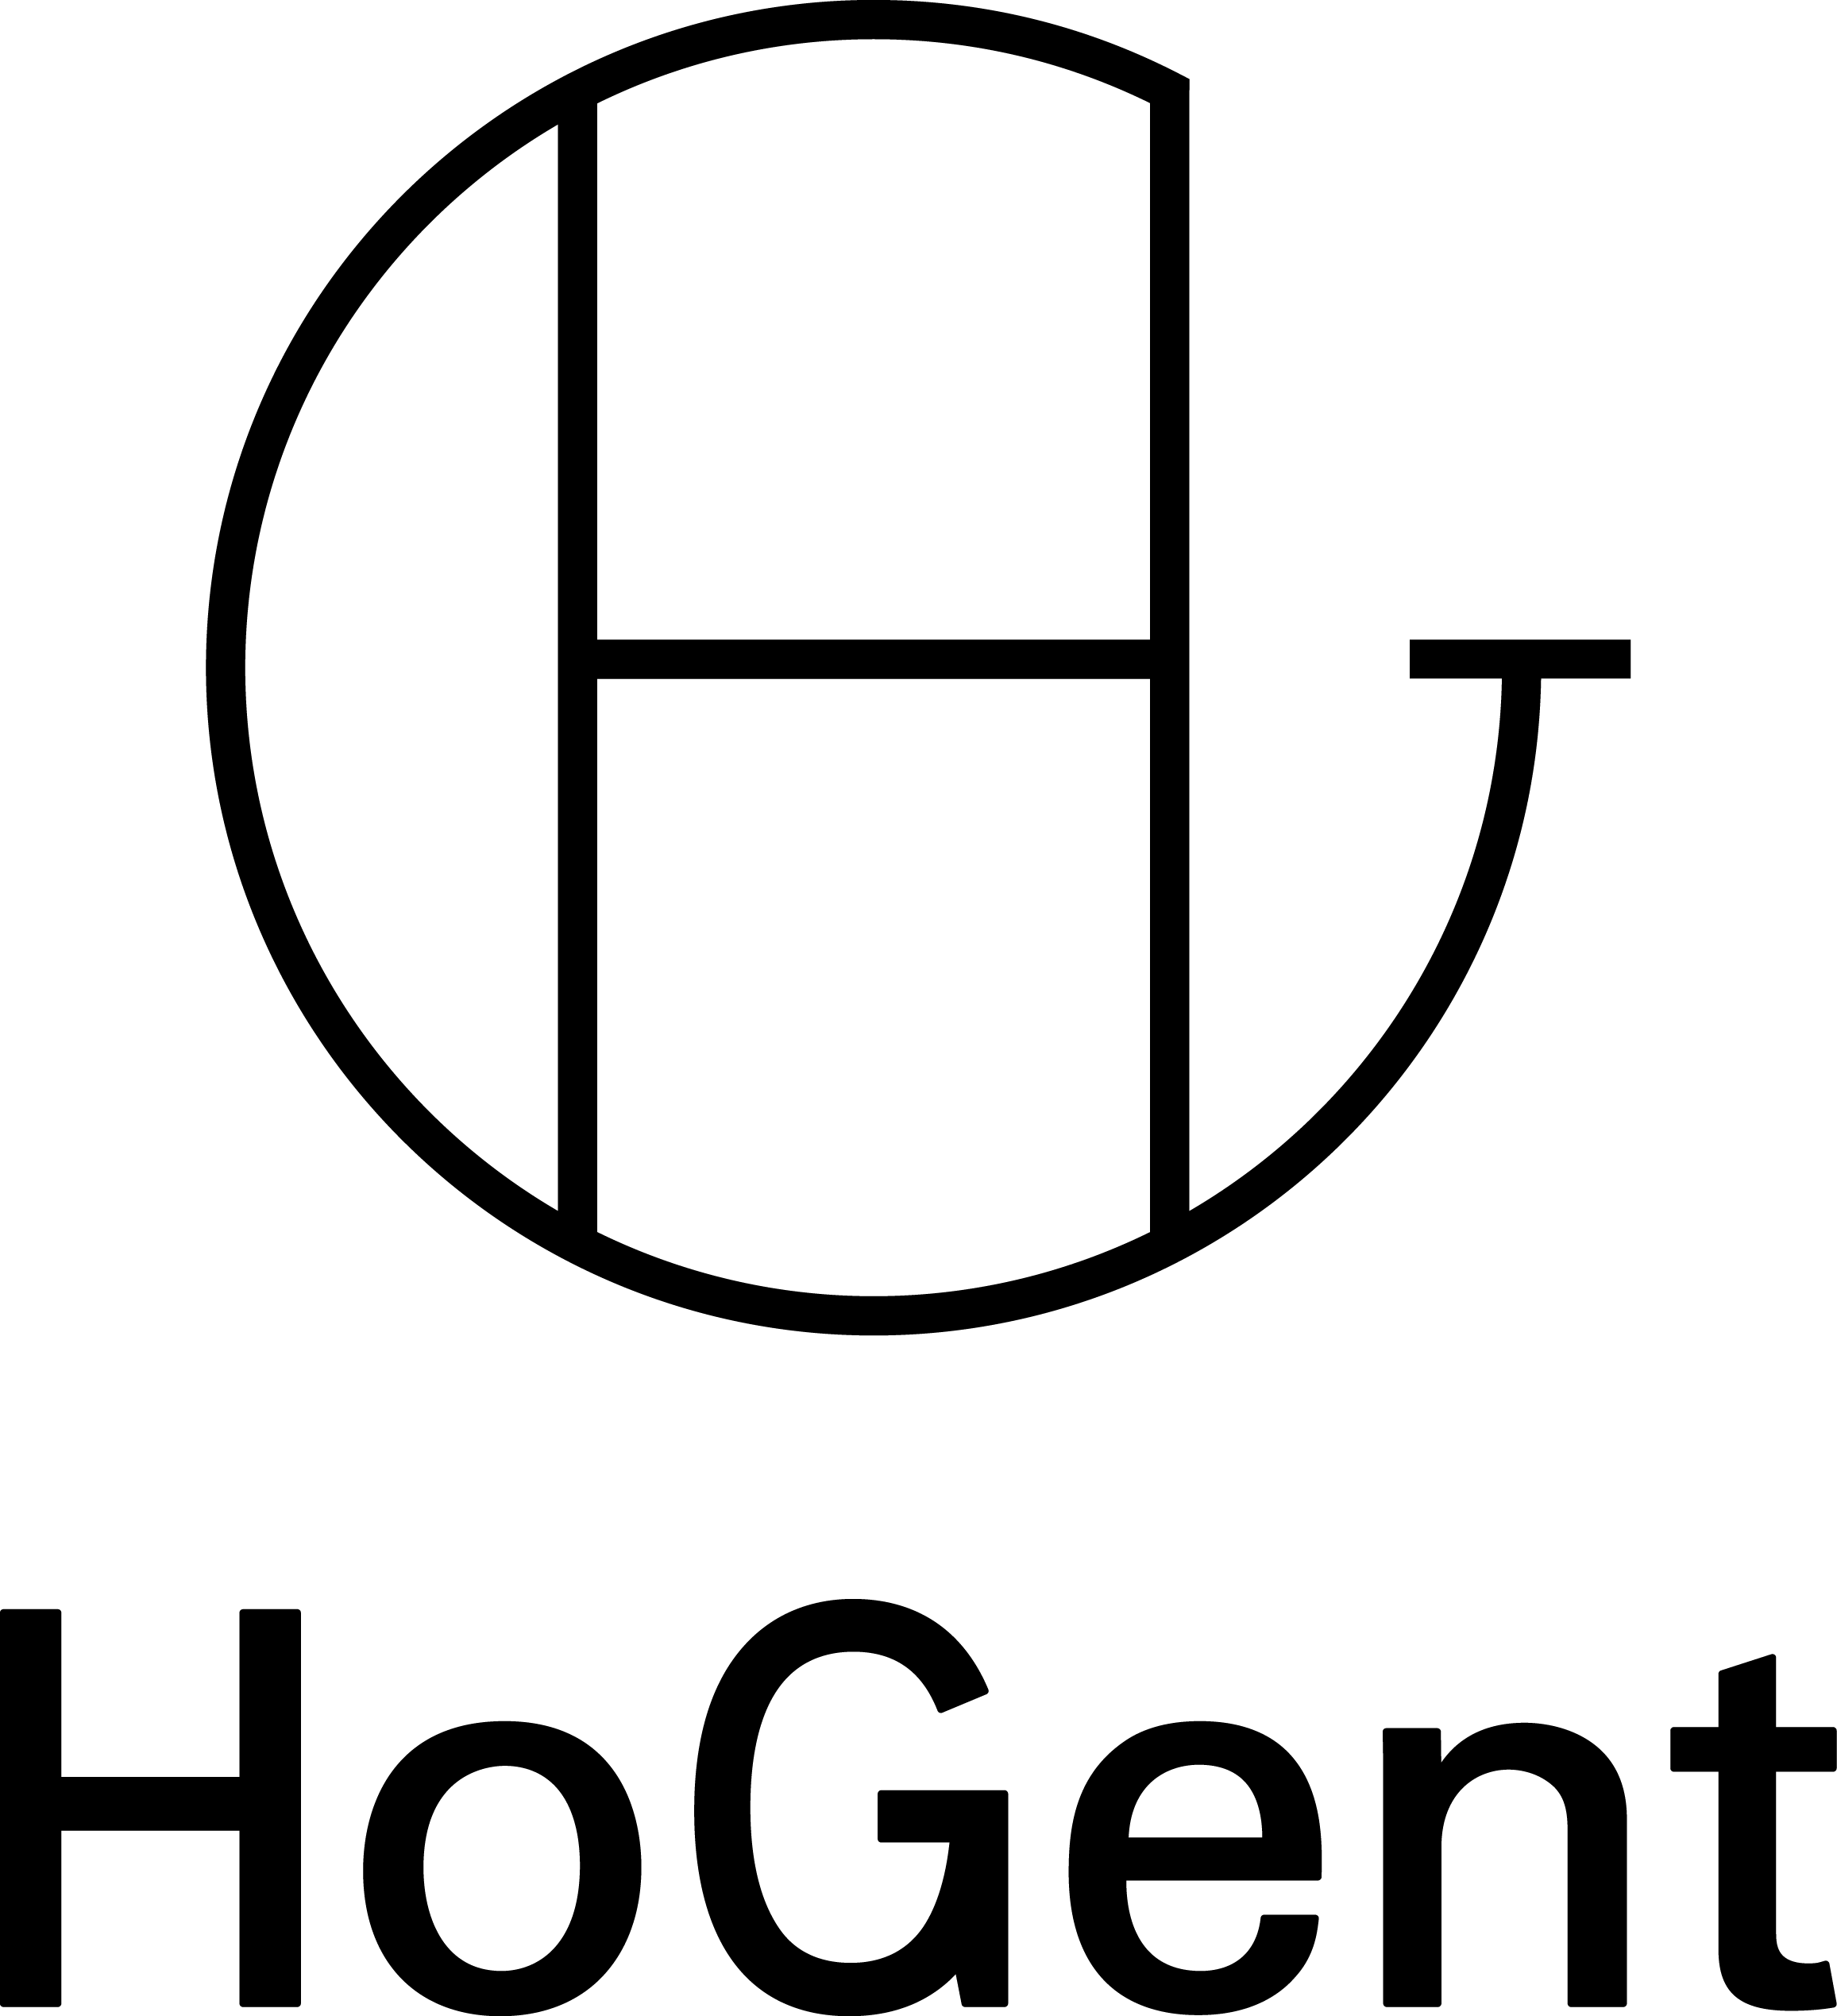
\includegraphics[width=2.5cm]{img/HG-beeldmerk-woordmerk}\\[.5cm]
    Faculteit Bedrijf en Organisatie\\[3cm]
    \titel
    \vfill
    \student\\[3.5cm]
    Scriptie voorgedragen tot het bekomen van de graad van\\professionele bachelor in de toegepaste informatica\\[2cm]
    Promotor:\\
    \promotor\\
    \ifdefempty{\copromotor}{\vspace{2.5cm}}{Co-promotor:\\\copromotor\\[2.5cm]}
    Instelling: \instelling\\[.5cm]
    Academiejaar: \academiejaar\\[.5cm]
    \ifcase \examenperiode \or Eerste \or Tweede \else Derde \fi examenperiode
    \endgroup

  \end{center}
  \restoregeometry
\end{titlepage}
  \emptypage
\begin{titlepage}
  \newgeometry{top=5.35cm,bottom=1.5cm,left=1.5cm,right=1.5cm}
  \begin{center}

    \begingroup
    \rmfamily
    \IfLanguageName{dutch}{Faculteit Bedrijf en Organisatie}{Faculty of Business and Information Management}\\[3cm]
    \titel
    \vfill
    \student\\[3.5cm]
    \IfLanguageName{dutch}{Scriptie voorgedragen tot het bekomen van de graad van\\professionele bachelor in de toegepaste informatica}{Thesis submitted in partial fulfilment of the requirements for the degree of\\professional bachelor of applied computer science}\\[2cm]
    Promotor:\\
    \promotor\\
    \ifdefempty{\copromotor}{\vspace{2.5cm}}{Co-promotor:\\\copromotor\\[2.5cm]}
    \IfLanguageName{dutch}{Instelling}{Institution}: \instelling\\[.5cm]
    \IfLanguageName{dutch}{Academiejaar}{Academic year}: \academiejaar\\[.5cm]
    \IfLanguageName{dutch}{%
    \ifcase \examenperiode \or Eerste \or Tweede \else Derde \fi examenperiode}{%
    \ifcase \examenperiode \or First \or Second \else Third \fi examination period}
    \endgroup

  \end{center}
  \restoregeometry
\end{titlepage}
}

%----------------------------------------------------------------------------------------
%	BIBLIOGRAPHY AND INDEX
%----------------------------------------------------------------------------------------

\usepackage[style=apa,backend=biber]{biblatex}
\usepackage{csquotes}
\DeclareLanguageMapping{dutch}{dutch-apa}
\addbibresource{bachproef-tin.bib} % BibTeX bibliography file
\addbibresource{../voorstel/voorstel.bib}
\defbibheading{bibempty}{}

\usepackage{calc} % For simpler calculation - used for spacing the index letter headings correctly
\usepackage{makeidx} % Required to make an index
\makeindex % Tells LaTeX to create the files required for indexing

%----------------------------------------------------------------------------------------
%	MAIN TABLE OF CONTENTS
%----------------------------------------------------------------------------------------

\usepackage{titletoc} % Required for manipulating the table of contents

\contentsmargin{0cm} % Removes the default margin

% Part text styling
\titlecontents{part}[0cm]
{\addvspace{20pt}\centering\large\bfseries}
{}
{}
{}

% Chapter text styling
\titlecontents{chapter}[1.25cm] % Indentation
{\addvspace{12pt}\large\sffamily\bfseries} % Spacing and font options for chapters
{\color{maincolor!60}\contentslabel[\Large\thecontentslabel]{1.25cm}\color{maincolor}} % Chapter number
{\color{maincolor}}
{\color{maincolor!60}\normalsize\;\titlerule*[.5pc]{.}\;\thecontentspage} % Page number

% Section text styling
\titlecontents{section}[1.25cm] % Indentation
{\addvspace{3pt}\sffamily\bfseries} % Spacing and font options for sections
{\contentslabel[\thecontentslabel]{1.25cm}} % Section number
{}
{\hfill\color{black}\thecontentspage} % Page number
[]

% Subsection text styling
\titlecontents{subsection}[1.25cm] % Indentation
{\addvspace{1pt}\sffamily\small} % Spacing and font options for subsections
{\contentslabel[\thecontentslabel]{1.25cm}} % Subsection number
{}
{\ \titlerule*[.5pc]{.}\;\thecontentspage} % Page number
[]

% List of figures
\titlecontents{figure}[0em]
{\addvspace{-5pt}\sffamily}
{\thecontentslabel\hspace*{1em}}
{}
{\ \titlerule*[.5pc]{.}\;\thecontentspage}
[]

% List of tables
\titlecontents{table}[0em]
{\addvspace{-5pt}\sffamily}
{\thecontentslabel\hspace*{1em}}
{}
{\ \titlerule*[.5pc]{.}\;\thecontentspage}
[]

%----------------------------------------------------------------------------------------
%	MINI TABLE OF CONTENTS IN PART HEADS
%----------------------------------------------------------------------------------------

% Chapter text styling
\titlecontents{lchapter}[0em] % Indenting
{\addvspace{15pt}\large\sffamily\bfseries} % Spacing and font options for chapters
{\color{maincolor}\contentslabel[\Large\thecontentslabel]{1.25cm}\color{maincolor}} % Chapter number
{}
{\color{maincolor}\normalsize\sffamily\bfseries\;\titlerule*[.5pc]{.}\;\thecontentspage} % Page number

% Section text styling
\titlecontents{lsection}[0em] % Indenting
{\sffamily\small} % Spacing and font options for sections
{\contentslabel[\thecontentslabel]{1.25cm}} % Section number
{}
{}

% Subsection text styling
\titlecontents{lsubsection}[.5em] % Indentation
{\normalfont\footnotesize\sffamily} % Font settings
{}
{}
{}

%----------------------------------------------------------------------------------------
%	PAGE HEADERS
%----------------------------------------------------------------------------------------

\usepackage{fancyhdr} % Required for header and footer configuration

\pagestyle{fancy}
\renewcommand{\chaptermark}[1]{\markboth{\sffamily\normalsize\bfseries\chaptername\ \thechapter.\ #1}{}} % Chapter text font settings
\renewcommand{\sectionmark}[1]{\markright{\sffamily\normalsize\thesection\hspace{5pt}#1}{}} % Section text font settings
\fancyhf{} \fancyhead[LE,RO]{\sffamily\normalsize\thepage} % Font setting for the page number in the header
\fancyhead[LO]{\rightmark} % Print the nearest section name on the left side of odd pages
\fancyhead[RE]{\leftmark} % Print the current chapter name on the right side of even pages
\renewcommand{\headrulewidth}{0.5pt} % Width of the rule under the header
\addtolength{\headheight}{2.5pt} % Increase the spacing around the header slightly
\renewcommand{\footrulewidth}{0pt} % Removes the rule in the footer
\fancypagestyle{plain}{\fancyhead{}\renewcommand{\headrulewidth}{0pt}} % Style for when a plain pagestyle is specified

% Removes the header from odd empty pages at the end of chapters
\makeatletter
\renewcommand{\cleardoublepage}{
\clearpage\ifodd\c@page\else
\hbox{}
\vspace*{\fill}
\thispagestyle{empty}
\newpage
\fi}

%----------------------------------------------------------------------------------------
%	THEOREM STYLES
%----------------------------------------------------------------------------------------

\usepackage{amsmath,amsfonts,amssymb,amsthm} % For math equations, theorems, symbols, etc

\newcommand{\intoo}[2]{\mathopen{]}#1\,;#2\mathclose{[}}
\newcommand{\ud}{\mathop{\mathrm{{}d}}\mathopen{}}
\newcommand{\intff}[2]{\mathopen{[}#1\,;#2\mathclose{]}}
\newtheorem{notation}{Notation}[chapter]

% Boxed/framed environments
\newtheoremstyle{maincolornumbox}% % Theorem style name
{0pt}% Space above
{0pt}% Space below
{\normalfont}% % Body font
{}% Indent amount
{\small\bf\sffamily\color{maincolor}}% % Theorem head font
{\;}% Punctuation after theorem head
{0.25em}% Space after theorem head
{\small\sffamily\color{maincolor}\thmname{#1}\nobreakspace\thmnumber{\@ifnotempty{#1}{}\@upn{#2}}% Theorem text (e.g. Theorem 2.1)
\thmnote{\nobreakspace\the\thm@notefont\sffamily\bfseries\color{black}---\nobreakspace#3.}} % Optional theorem note
\renewcommand{\qedsymbol}{$\blacksquare$}% Optional qed square

\newtheoremstyle{blacknumex}% Theorem style name
{5pt}% Space above
{5pt}% Space below
{\normalfont}% Body font
{} % Indent amount
{\small\bf\sffamily}% Theorem head font
{\;}% Punctuation after theorem head
{0.25em}% Space after theorem head
{\small\sffamily{\tiny\ensuremath{\blacksquare}}\nobreakspace\thmname{#1}\nobreakspace\thmnumber{\@ifnotempty{#1}{}\@upn{#2}}% Theorem text (e.g. Theorem 2.1)
\thmnote{\nobreakspace\the\thm@notefont\sffamily\bfseries---\nobreakspace#3.}}% Optional theorem note

\newtheoremstyle{blacknumbox} % Theorem style name
{0pt}% Space above
{0pt}% Space below
{\normalfont}% Body font
{}% Indent amount
{\small\bf\sffamily}% Theorem head font
{\;}% Punctuation after theorem head
{0.25em}% Space after theorem head
{\small\sffamily\thmname{#1}\nobreakspace\thmnumber{\@ifnotempty{#1}{}\@upn{#2}}% Theorem text (e.g. Theorem 2.1)
\thmnote{\nobreakspace\the\thm@notefont\sffamily\bfseries---\nobreakspace#3.}}% Optional theorem note

% Non-boxed/non-framed environments
\newtheoremstyle{maincolornum}% % Theorem style name
{5pt}% Space above
{5pt}% Space below
{\normalfont}% % Body font
{}% Indent amount
{\small\bf\sffamily\color{maincolor}}% % Theorem head font
{\;}% Punctuation after theorem head
{0.25em}% Space after theorem head
{\small\sffamily\color{maincolor}\thmname{#1}\nobreakspace\thmnumber{\@ifnotempty{#1}{}\@upn{#2}}% Theorem text (e.g. Theorem 2.1)
\thmnote{\nobreakspace\the\thm@notefont\sffamily\bfseries\color{black}---\nobreakspace#3.}} % Optional theorem note
\renewcommand{\qedsymbol}{$\blacksquare$}% Optional qed square
\makeatother

% Defines the theorem text style for each type of theorem to one of the three styles above
\newcounter{dummy}
\numberwithin{dummy}{section}
\theoremstyle{maincolornumbox}
\newtheorem{theoremeT}[dummy]{Theorem}
\newtheorem{problem}{Problem}[chapter]
\newtheorem{exerciseT}{Exercise}[chapter]
\theoremstyle{blacknumex}
\newtheorem{exampleT}{Example}[chapter]
\theoremstyle{blacknumbox}
\newtheorem{vocabulary}{Vocabulary}[chapter]
\newtheorem{definitionT}{Definition}[section]
\newtheorem{corollaryT}[dummy]{Corollary}
\theoremstyle{maincolornum}
\newtheorem{proposition}[dummy]{Proposition}

%----------------------------------------------------------------------------------------
%	DEFINITION OF COLORED BOXES
%----------------------------------------------------------------------------------------

\RequirePackage[framemethod=default]{mdframed} % Required for creating the theorem, definition, exercise and corollary boxes

% Theorem box
\newmdenv[skipabove=7pt,
skipbelow=7pt,
backgroundcolor=black!5,
linecolor=maincolor,
innerleftmargin=5pt,
innerrightmargin=5pt,
innertopmargin=5pt,
leftmargin=0cm,
rightmargin=0cm,
innerbottommargin=5pt]{tBox}

% Exercise box
\newmdenv[skipabove=7pt,
skipbelow=7pt,
rightline=false,
leftline=true,
topline=false,
bottomline=false,
backgroundcolor=maincolor!10,
linecolor=maincolor,
innerleftmargin=5pt,
innerrightmargin=5pt,
innertopmargin=5pt,
innerbottommargin=5pt,
leftmargin=0cm,
rightmargin=0cm,
linewidth=4pt]{eBox}

% Definition box
\newmdenv[skipabove=7pt,
skipbelow=7pt,
rightline=false,
leftline=true,
topline=false,
bottomline=false,
linecolor=maincolor,
innerleftmargin=5pt,
innerrightmargin=5pt,
innertopmargin=0pt,
leftmargin=0cm,
rightmargin=0cm,
linewidth=4pt,
innerbottommargin=0pt]{dBox}

% Corollary box
\newmdenv[skipabove=7pt,
skipbelow=7pt,
rightline=false,
leftline=true,
topline=false,
bottomline=false,
linecolor=gray,
backgroundcolor=black!5,
innerleftmargin=5pt,
innerrightmargin=5pt,
innertopmargin=5pt,
leftmargin=0cm,
rightmargin=0cm,
linewidth=4pt,
innerbottommargin=5pt]{cBox}

% Creates an environment for each type of theorem and assigns it a theorem text style from the "Theorem Styles" section above and a colored box from above
\newenvironment{theorem}{\begin{tBox}\begin{theoremeT}}{\end{theoremeT}\end{tBox}}
\newenvironment{exercise}{\begin{eBox}\begin{exerciseT}}{\hfill{\color{maincolor}\tiny\ensuremath{\blacksquare}}\end{exerciseT}\end{eBox}}
\newenvironment{definition}{\begin{dBox}\begin{definitionT}}{\end{definitionT}\end{dBox}}
\newenvironment{example}{\begin{exampleT}}{\hfill{\tiny\ensuremath{\blacksquare}}\end{exampleT}}
\newenvironment{corollary}{\begin{cBox}\begin{corollaryT}}{\end{corollaryT}\end{cBox}}

%----------------------------------------------------------------------------------------
%	REMARK ENVIRONMENT
%----------------------------------------------------------------------------------------

\newenvironment{remark}{\par\vspace{10pt}\small % Vertical white space above the remark and smaller font size
\begin{list}{}{
\leftmargin=35pt % Indentation on the left
\rightmargin=25pt}\item\ignorespaces % Indentation on the right
\makebox[-2.5pt]{\begin{tikzpicture}[overlay]
\node[draw=maincolor!60,line width=1pt,circle,fill=maincolor!25,font=\sffamily\bfseries,inner sep=2pt,outer sep=0pt] at (-15pt,0pt){\textcolor{maincolor}{R}};\end{tikzpicture}} % Orange R in a circle
\advance\baselineskip -1pt}{\end{list}\vskip5pt} % Tighter line spacing and white space after remark

%----------------------------------------------------------------------------------------
%	SECTION NUMBERING IN THE MARGIN
%----------------------------------------------------------------------------------------

\makeatletter
\renewcommand{\@seccntformat}[1]{\llap{\textcolor{maincolor}{\csname the#1\endcsname}\hspace{1em}}}
\renewcommand{\section}{\@startsection{section}{1}{\z@}
{-4ex \@plus -1ex \@minus -.4ex}
{1ex \@plus.2ex }
{\normalfont\large\sffamily\bfseries}}
\renewcommand{\subsection}{\@startsection {subsection}{2}{\z@}
{-3ex \@plus -0.1ex \@minus -.4ex}
{0.5ex \@plus.2ex }
{\normalfont\sffamily\bfseries}}
\renewcommand{\subsubsection}{\@startsection {subsubsection}{3}{\z@}
{-2ex \@plus -0.1ex \@minus -.2ex}
{.2ex \@plus.2ex }
{\normalfont\small\sffamily\bfseries}}
\renewcommand\paragraph{\@startsection{paragraph}{4}{\z@}
{-2ex \@plus-.2ex \@minus .2ex}
{.1ex}
{\normalfont\small\sffamily\bfseries}}

%----------------------------------------------------------------------------------------
%	PART HEADINGS
%----------------------------------------------------------------------------------------

% numbered part in the table of contents
\newcommand{\@mypartnumtocformat}[2]{%
\setlength\fboxsep{0pt}%
\noindent\colorbox{maincolor!20}{\strut\parbox[c][.7cm]{\ecart}{\color{maincolor!70}\Large\sffamily\bfseries\centering#1}}\hskip\esp\colorbox{maincolor!40}{\strut\parbox[c][.7cm]{\linewidth-\ecart-\esp}{\Large\sffamily\centering#2}}}%
%%%%%%%%%%%%%%%%%%%%%%%%%%%%%%%%%%
% unnumbered part in the table of contents
\newcommand{\@myparttocformat}[1]{%
\setlength\fboxsep{0pt}%
\noindent\colorbox{maincolor!40}{\strut\parbox[c][.7cm]{\linewidth}{\Large\sffamily\centering#1}}}%
%%%%%%%%%%%%%%%%%%%%%%%%%%%%%%%%%%
\newlength\esp
\setlength\esp{4pt}
\newlength\ecart
\setlength\ecart{1.2cm-\esp}
\newcommand{\thepartimage}{}%
\newcommand{\partimage}[1]{\renewcommand{\thepartimage}{#1}}%
\def\@part[#1]#2{%
\ifnum \c@secnumdepth >-2\relax%
\refstepcounter{part}%
\addcontentsline{toc}{part}{\texorpdfstring{\protect\@mypartnumtocformat{\thepart}{#1}}{\partname~\thepart\ ---\ #1}}
\else%
\addcontentsline{toc}{part}{\texorpdfstring{\protect\@myparttocformat{#1}}{#1}}%
\fi%
\startcontents%
\markboth{}{}%
{\thispagestyle{empty}%
\begin{tikzpicture}[remember picture,overlay]%
\node at (current page.north west){\begin{tikzpicture}[remember picture,overlay]%
\fill[maincolor!20](0cm,0cm) rectangle (\paperwidth,-\paperheight);
\node[anchor=north] at (4cm,-3.25cm){\color{maincolor!40}\fontsize{220}{100}\sffamily\bfseries\@Roman\c@part};
\node[anchor=south east] at (\paperwidth-1cm,-\paperheight+1cm){\parbox[t][][t]{8.5cm}{
\printcontents{l}{0}{\setcounter{tocdepth}{1}}%
}};
\node[anchor=north east] at (\paperwidth-1.5cm,-3.25cm){\parbox[t][][t]{15cm}{\strut\raggedleft\color{white}\fontsize{30}{30}\sffamily\bfseries#2}};
\end{tikzpicture}};
\end{tikzpicture}}%
\@endpart}
\def\@spart#1{%
\startcontents%
\phantomsection
{\thispagestyle{empty}%
\begin{tikzpicture}[remember picture,overlay]%
\node at (current page.north west){\begin{tikzpicture}[remember picture,overlay]%
\fill[maincolor!20](0cm,0cm) rectangle (\paperwidth,-\paperheight);
\node[anchor=north east] at (\paperwidth-1.5cm,-3.25cm){\parbox[t][][t]{15cm}{\strut\raggedleft\color{white}\fontsize{30}{30}\sffamily\bfseries#1}};
\end{tikzpicture}};
\end{tikzpicture}}
\addcontentsline{toc}{part}{\texorpdfstring{%
\setlength\fboxsep{0pt}%
\noindent\protect\colorbox{maincolor!40}{\strut\protect\parbox[c][.7cm]{\linewidth}{\Large\sffamily\protect\centering #1\quad\mbox{}}}}{#1}}%
\@endpart}
\def\@endpart{\vfil\newpage
\if@twoside
\if@openright
\null
\thispagestyle{empty}%
\newpage
\fi
\fi
\if@tempswa
\twocolumn
\fi}

%----------------------------------------------------------------------------------------
%	CHAPTER HEADINGS
%----------------------------------------------------------------------------------------

% A switch to conditionally include a picture, implemented by  Christian Hupfer
\newif\ifusechapterimage
\usechapterimagetrue
\newcommand{\thechapterimage}{}%
\newcommand{\chapterimage}[1]{\ifusechapterimage\renewcommand{\thechapterimage}{#1}\fi}%
\def\@makechapterhead#1{%
{\parindent \z@ \raggedright \normalfont
\ifnum \c@secnumdepth >\m@ne
\if@mainmatter
\begin{tikzpicture}[remember picture,overlay]
\node at (current page.north west)
{\begin{tikzpicture}[remember picture,overlay]
\node[anchor=north west,inner sep=0pt] at (0,0) {\ifusechapterimage\includegraphics[width=\paperwidth]{\thechapterimage}\fi};
\draw[anchor=west] (\Gm@lmargin,-9cm) node [line width=2pt,rounded corners=15pt,draw=maincolor,fill=white,fill opacity=0.5,inner sep=15pt]{\strut\makebox[22cm]{}};
\draw[anchor=west] (\Gm@lmargin+.3cm,-9cm) node {\huge\sffamily\bfseries\color{black}\thechapter. #1\strut};
\end{tikzpicture}};
\end{tikzpicture}
\else
\begin{tikzpicture}[remember picture,overlay]
\node at (current page.north west)
{\begin{tikzpicture}[remember picture,overlay]
\node[anchor=north west,inner sep=0pt] at (0,0) {\ifusechapterimage\includegraphics[width=\paperwidth]{\thechapterimage}\fi};
\draw[anchor=west] (\Gm@lmargin,-9cm) node [line width=2pt,rounded corners=15pt,draw=maincolor,fill=white,fill opacity=0.5,inner sep=15pt]{\strut\makebox[22cm]{}};
\draw[anchor=west] (\Gm@lmargin+.3cm,-9cm) node {\huge\sffamily\bfseries\color{black}#1\strut};
\end{tikzpicture}};
\end{tikzpicture}
\fi\fi\par\vspace*{270\p@}}}

%-------------------------------------------

\def\@makeschapterhead#1{%
\begin{tikzpicture}[remember picture,overlay]
\node at (current page.north west)
{\begin{tikzpicture}[remember picture,overlay]
\node[anchor=north west,inner sep=0pt] at (0,0) {\ifusechapterimage\includegraphics[width=\paperwidth]{\thechapterimage}\fi};
\draw[anchor=west] (\Gm@lmargin,-9cm) node [line width=2pt,rounded corners=15pt,draw=maincolor,fill=white,fill opacity=0.5,inner sep=15pt]{\strut\makebox[22cm]{}};
\draw[anchor=west] (\Gm@lmargin+.3cm,-9cm) node {\huge\sffamily\bfseries\color{black}#1\strut};
\end{tikzpicture}};
\end{tikzpicture}
\par\vspace*{270\p@}}
\makeatother

%----------------------------------------------------------------------------------------
%	HYPERLINKS IN THE DOCUMENTS
%----------------------------------------------------------------------------------------

\usepackage{hyperref}
\hypersetup{hidelinks,backref=true,pagebackref=true,hyperindex=true,colorlinks=false,breaklinks=true,urlcolor= maincolor,bookmarks=true,bookmarksopen=false,pdftitle={Title},pdfauthor={Author}}
\usepackage{bookmark}
\bookmarksetup{
open,
numbered,
addtohook={%
\ifnum\bookmarkget{level}=0 % chapter
\bookmarksetup{bold}%
\fi
\ifnum\bookmarkget{level}=-1 % part
\bookmarksetup{color=maincolor,bold}%
\fi
}
}

%----------------------------------------------------------------------------------------
%	Java source code
%----------------------------------------------------------------------------------------

% Commando voor invoegen Java-broncodebestanden (dank aan Niels Corneille)
% Gebruik:
%   \codefragment{source/MijnKlasse.java}{Uitleg bij de code}
%
% Je kan dit aanpassen aan de taal die je zelf het meeste gebruikt in je
% bachelorproef.
\newcommand{\codefragment}[2]{ \lstset{%
  language=java,
  breaklines=true,
  float=th,
  caption={#2},
  basicstyle=\scriptsize,
  frame=single,
  extendedchars=\true
}
\lstinputlisting{#1}}

% Leeg blad
\newcommand{\emptypage}{%
\newpage
\thispagestyle{empty}
\mbox{}
\newpage
}


%%---------- Documenteigenschappen --------------------------------------------

% Je eigen naam
\newcommand{\student}{Lennert Mertens}

% De naam van je promotor (lector van de opleiding)
\newcommand{\promotor}{Steven Van Impe}

% De naam van je co-promotor. Als je promotor ook je opdrachtgever is en je
% dus ook inhoudelijk begeleidt (en enkel dan!), mag je dit leeg laten.
\newcommand{\copromotor}{Pieter-Jan Saveyn}

% Indien je bachelorproef in opdracht van/in samenwerking met een bedrijf of
% externe organisatie geschreven is, geef je hier de naam. Zoniet laat je dit
% zoals het is.
\newcommand{\instelling}{Nubera}

% De titel van het rapport/bachelorproef
\newcommand{\titel}{Onderzoek naar serverless computing en open source serverless infrastructuur: vergelijkende studie en Proof of Concept}

% Datum van indienen (gebruik telkens de deadline, ook al geef je eerder af)
\newcommand{\datum}{31 mei 2019}

% Academiejaar
\newcommand{\academiejaar}{2018-2019}

% Examenperiode
%  - 1e semester = 1e examenperiode => 1
%  - 2e semester = 2e examenperiode => 2
%  - tweede zit  = 3e examenperiode => 3
\newcommand{\examenperiode}{2}

%%=============================================================================
%% Inhoud document
%%=============================================================================

\begin{document}

%---------- Taalselectie ------------------------------------------------------
% Als je je bachelorproef in het Engels schrijft, haal dan onderstaande regel
% uit commentaar. Let op: de tekst op de voorkaft blijft in het Nederlands, en
% dat is ook de bedoeling!

%\selectlanguage{english}

%---------- Titelblad ---------------------------------------------------------
\inserttitlepage

%---------- Samenvatting, voorwoord -------------------------------------------
\usechapterimagefalse
%%=============================================================================
%% Voorwoord
%%=============================================================================

\chapter*{Woord vooraf}
\label{ch:voorwoord}

%% TODO:
%% Het voorwoord is het enige deel van de bachelorproef waar je vanuit je
%% eigen standpunt (``ik-vorm'') mag schrijven. Je kan hier bv. motiveren
%% waarom jij het onderwerp wil bespreken.
%% Vergeet ook niet te bedanken wie je geholpen/gesteund/... heeft

Deze bachelorproef werd geschreven in het kader van het behalen van de graad Bachelor in toegepaste informatica.

%%=============================================================================
%% Samenvatting
%%=============================================================================

% TODO: De "abstract" of samenvatting is een kernachtige (~ 1 blz. voor een
% thesis) synthese van het document.
%
% Deze aspecten moeten zeker aan bod komen:
% - Context: waarom is dit werk belangrijk?
% - Nood: waarom moest dit onderzocht worden?
% - Taak: wat heb je precies gedaan?
% - Object: wat staat in dit document geschreven?
% - Resultaat: wat was het resultaat?
% - Conclusie: wat is/zijn de belangrijkste conclusie(s)?
% - Perspectief: blijven er nog vragen open die in de toekomst nog kunnen
%    onderzocht worden? Wat is een mogelijk vervolg voor jouw onderzoek?
%
% LET OP! Een samenvatting is GEEN voorwoord!

%%---------- Nederlandse samenvatting -----------------------------------------
%
% TODO: Als je je bachelorproef in het Engels schrijft, moet je eerst een
% Nederlandse samenvatting invoegen. Haal daarvoor onderstaande code uit
% commentaar.
% Wie zijn bachelorproef in het Nederlands schrijft, kan dit negeren, de inhoud
% wordt niet in het document ingevoegd.
\chapter*{Samenvatting}
Serverless computing is een ''hot topic'' en kent een grote opmars binnen de IT wereld. Verschillende bedrijven hebben deze technologie reeds geadopteerd en in de toekomst zullen er nog heel veel volgen. Omdat de strijd binnen de serverless wereld nog niet gestreden is en er nog geen standaard is gezet, is een onderzoek naar veelbelovende open source serverless oplossingen zinvol. Nubera is op zoek naar een open source serverless framework, dat aanleunt bij hun requirements, om aan te bieden bij klanten die serverless willen gaan werken. Nubera gaf aan interesse te hebben in Fission en zocht hiervoor een veelbelovend alternatief. 
\\\\
Vertrekkend vanuit een gedetailleerde literatuurstudie die de theorie omtrent serverless en alle bijkomstigheden behandelt, werden in samenspraak met Nubera requirements gecapteerd. Op basis van de requirements wordt in de uitwerking, aan de hand van een oplijsting, een interessant open source framework gekozen en vergeleken met Fission. OpenFaaS blijkt het beste alternatief te zijn voor Fission conform aan de opgestelde requirements. Beide frameworks worden aan de hand van een Proof of Concept met elkaar vergeleken om hieruit een aanbeveling voor Nubera te kunnen vormen. 
\\\\
Vanuit de Proof of Concept en vergelijkende studie komt OpenFaaS naar voor als het meest veelbelovend open source serverless framework dat aanleunt bij de requirements van Nubera.
\\\\
Aangezien serverless computing nog in de kinderschoenen staat en er heel wat open source frameworks in ontwikkeling zijn, is het zinvol onderzoek te doen naar anderen alternatieven deze en te vergelijken met de frameworks die in dit onderzoek werden behandeld. Deze bachelorproef vormt een aanzet zijn voor een vergelijkende studie tussen meer open source serverless frameworks.


%---------- Inhoudstafel ------------------------------------------------------
\pagestyle{empty} % No headers
\tableofcontents % Print the table of contents itself
\cleardoublepage % Forces the first chapter to start on an odd page so it's on the right
\pagestyle{fancy} % Print headers again

%---------- Lijst figuren, afkortingen, ... -----------------------------------

% Indien gewenst kan je hier een lijst van figuren/tabellen opgeven. Geef in
% dat geval je figuren/tabellen altijd een korte beschrijving:
%
%  \caption[korte beschrijving]{uitgebreide beschrijving}

\listoffigures
\listoftables

% Als je een lijst van afkortingen of termen wil toevoegen, dan hoort die
% hier thuis. Gebruik bijvoorbeeld de ``glossaries'' package.
% https://www.sharelatex.com/learn/Glossaries

%%---------- Kern -------------------------------------------------------------

%%=============================================================================
%% Inleiding
%%=============================================================================

\chapter{Inleiding}
\label{ch:inleiding}

%%De inleiding moet de lezer net genoeg informatie verschaffen om het onderwerp te begrijpen en in te zien waarom de onderzoeksvraag de moeite waard is om te onderzoeken. In de inleiding ga je literatuurverwijzingen beperken, zodat de tekst vlot leesbaar blijft. Je kan de inleiding verder onderverdelen in secties als dit de tekst verduidelijkt. Zaken die aan bod kunnen komen in de inleiding~\autocite{Pollefliet2011}:%%
Cloud Computing technologie is alomtegenwoordig, er bestaan verschillende benaderingen met elk hun specifieke eigenschappen, voor- en nadelen. Meer en meer bedrijven zijn reeds begonnen met migratie van resources naar de Cloud en dit biedt een variëteit aan mogelijkheden. Grote cloud providers zoals Google Cloud Platform, Amazon Web Services (AWS), Microsoft Azure en IBM bieden hun klanten al heel wat mogelijkheden aan om gebruik te maken van cloud-diensten. Vele bedrijven verkiezen toch nog steeds een eigen infrastructuur boven het toevertrouwen van resources aan grote cloud providers zoals hierboven genoemd. Klassieke bedrijven waar informatie confidentieel is hebben toch enige argwaan om zomaar alles in de publieke cloud te draaien. Bedrijven die enige afstand willen nemen van de publieke cloud kunnen toch meegenieten van de veelzijdige mogelijkheden dat cloud computing met zich meebrengt. Het is mogelijk voor bedrijven om gebruik te maken van software zoals VMWare, Microsoft Cloud, IBM Bluemix Cloud om zo een eigen cloud infrastructuur op te zetten op locatie of in een private cloud. Deze benadering biedt bedrijven, die mee willen groeien in het hele cloud gebeuren maar niet willen migreren naar de publieke cloud, toch de mogelijkheid mee te evolueren.
\\\\

De jongste jaren is er een nieuwe trend in Cloud computing geëvolueerd, namelijk serverless of vaak gerefereerd als Function-as-a-Service. Serverless technologie biedt heel wat voordelen op basis van verschillende aspecten. Serverless neemt overhead weg bij softwareontwikkelaars en stelt hun in staat enkel te focussen op wat er voor hen het meest toe doet, namelijk de software zelf.
\\\\

Deze studie behandelt enerzijds een uiteenzetting van de basis Cloud computing principes. Er wordt ook onderzoek gedaan naar wat serverless precies inhoudt, wat de voor- en nadelen zijn en welke componenten serverless mogelijk maken. De theoretische omschrijving van dit concept wordt geïllustreerd aan de hand van voorbeelden om zo de architectuur op een eenvoudige manier over te brengen. Daarnaast wordt op basis van verschillende requirements een overweging gemaakt voor het kiezen van twee open-source frameworks die de mogelijkheden aanbieden serverless te draaien op locatie. Het onderzoek wordt gestaafd met een proof-of-concept die twee frameworks vergelijkt.

%%\begin{itemize}
%%  \item context, achtergrond
%%  \item afbakenen van het onderwerp
%%  \item verantwoording van het onderwerp, methodologie
%%  \item probleemstelling
%%  \item onderzoeksdoelstelling
%%  \item onderzoeksvraag
%%  \item \ldots
%%\end{itemize}

\section{Probleemstelling}
\label{sec:probleemstelling}

%%Uit je probleemstelling moet duidelijk zijn dat je onderzoek een meerwaarde heeft voor een concrete doelgroep. De doelgroep moet goed gedefinieerd en afgelijnd zijn. Doelgroepen als ``bedrijven,'' ``KMO's,'' systeembeheerders, enz.~zijn nog te vaag. Als je een lijstje kan maken van de personen/organisaties die een meerwaarde zullen vinden in deze bachelorproef (dit is eigenlijk je steekproefkader), dan is dat een indicatie dat de doelgroep goed gedefinieerd is. Dit kan een enkel bedrijf zijn of zelfs één persoon (je co-promotor/opdrachtgever).%%

Er zijn bedrijven die interesse hebben in het gebruik van serverless omgevingen maar opteren om deze niet te draaien bij grote Cloud providers zoals Google, Amazon of Microsoft Azure. Bedrijven die serverless willen werken in hun eigen datacenter, de private cloud of op locatie hebben nood aan een framework dat hen in staat stelt dit te doen. Nubera heeft klanten die argwanend zijn wanneer ze voorstellen een Cloud omgeving op te zetten bij een van de grote spelers. Omdat nubera momenteel nog geen oplossing gebruikt om serverless te implementeren bij klanten op locatie werd mij gevraagd hiernaar onderzoek te doen en twee mogelijke frameworks te behandelen die voldoen aan vooropgestelde requirements. Er wordt een reproduceerbare proof-of-concept uitgewerkt die inzicht geeft in de behandelde frameworks.

\section{Onderzoeksvraag}
\label{sec:onderzoeksvraag}

%%Wees zo concreet mogelijk bij het formuleren van je onderzoeksvraag. Een onderzoeksvraag is trouwens iets waar nog niemand op dit moment een antwoord heeft (voor zover je kan nagaan). Het opzoeken van bestaande informatie (bv. ``welke tools bestaan er voor deze toepassing?'') is dus geen onderzoeksvraag. Je kan de onderzoeksvraag verder specifiëren in deelvragen. Bv.~als je onderzoek gaat over performantiemetingen, dan%%

Onderzoeksvraag: 
\begin{itemize}
    \item Wat omvat serverless infrastructuren en welke mogelijkheden biden open-source projecten die op locatie worden gedraaid?
\end{itemize}

Deelonderzoeksvragen: 
\begin{itemize}
    \item Wat is Cloud computing?
    \item Wat is serverless?
    \item Wat is de rol van onderliggende componenten (containers, microservices)?
    \item Wat zijn de voor-en nadelen van serverless infrastructuur?
    \item Wat is het verschil met traditionele infrastructuren?
    \item Welke voordelen biedt Fission ten opzichte van Open-FaaS of vice-versa?
    \item Welke meerwaarde bieden de open-source benaderingen ten opzichte van serverless platformen bij grote spelers?
\end{itemize}

Voorwaarden: 
\begin{itemize}
    \item Het onderdeel stand van zaken vormt een begrijpbare uiteenzetting van enkele basisconcepten en geeft een breed beeld over serverless en alle bijkomstigheden
    \item Onderzoek wordt gestaafd door een proof-of-concept van  twee interessante open-source frameworks die  Nubera zou kunnen gebruiken in serverless oplossingen op locatie
    \item Het opzetten van de omgeving is reproduceerbaar en is duidelijk gedocumenteerd
\end{itemize}



\section{Onderzoeksdoelstelling}
\label{sec:onderzoeksdoelstelling}

%%Wat is het beoogde resultaat van je bachelorproef? Wat zijn de criteria voor succes? Beschrijf die zo concreet mogelijk.%%
Deze bachlorproef moet kunnen fungeren als een rode draad voor het evolueren naar serverless infrastructuur. Het onderzoek biedt inzicht in open-source oplossingen die op locatie kunnen worden opgezet voor bedrijven die opteren om gebruik te maken van eigen infrastructuur of de private Cloud. Deze gids heeft een meerwaarde voor Nubera omdat ze op basis van verschillende requirements een overweging kunnen maken welk framework het interessantst is. Het onderzoek moet voldoende inzichten geven zodat de volledige bachelorproef voor iedereen begrijpbaar is, ook voor mensen met weinig Cloud computing ervaring.


\section{Opzet van deze bachelorproef}
\label{sec:opzet-bachelorproef}

% Het is gebruikelijk aan het einde van de inleiding een overzicht te
% geven van de opbouw van de rest van de tekst. Deze sectie bevat al een aanzet
% die je kan aanvullen/aanpassen in functie van je eigen tekst.

De rest van deze bachelorproef is als volgt opgebouwd:

In Hoofdstuk~\ref{ch:stand-van-zaken} wordt een overzicht gegeven van de stand van zaken binnen het onderzoeksdomein, op basis van een literatuurstudie.

In Hoofdstuk~\ref{ch:methodologie} wordt de methodologie toegelicht en worden de gebruikte onderzoekstechnieken besproken om een antwoord te kunnen formuleren op de onderzoeksvragen.

% TODO: Vul hier aan voor je eigen hoofstukken, één of twee zinnen per hoofdstuk
In Hoofdstuk~\ref{ch:uitwerking} worden op basis van enkele requirements opgelegd door Nubera twee interessante open-source frameworks gekozen voor het draaien van een serverless infrastrucctuur on-premises of in de private cloud.


In Hoofdstuk~\ref{ch:conclusie}, tenslotte, wordt de conclusie gegeven en een antwoord geformuleerd op de onderzoeksvragen. Daarbij wordt ook een aanzet gegeven voor toekomstig onderzoek binnen dit domein.


\chapter{Stand van zaken}
\label{ch:stand-van-zaken}

% Tip: Begin elk hoofdstuk met een paragraaf inleiding die beschrijft hoe
% dit hoofdstuk past binnen het geheel van de bachelorproef. Geef in het
% bijzonder aan wat de link is met het vorige en volgende hoofdstuk.

% Pas na deze inleidende paragraaf komt de eerste sectiehoofding.

%Dit hoofdstuk bevat je literatuurstudie. De inhoud gaat verder op de inleiding, maar zal het onderwerp van de bachelorproef *diepgaand* uitspitten. De bedoeling is dat de lezer na lezing van dit hoofdstuk helemaal op de hoogte is van de huidige stand van zaken (state-of-the-art) in het onderzoeksdomein. Iemand die niet vertrouwd is met het onderwerp, weet er nu voldoende om de rest van het verhaal te kunnen volgen, zonder dat die er nog andere informatie moet over opzoeken \autocite{Pollefliet2011}.
%
%Je verwijst bij elke bewering die je doet, vakterm die je introduceert, enz. naar je bronnen. In \LaTeX{} kan dat met het commando \texttt{$\backslash${textcite\{\}}} of \texttt{$\backslash${autocite\{\}}}. Als argument van het commando geef je de ``sleutel'' van een ``record'' in een bibliografische databank in het Bib\TeX{}-formaat (een tekstbestand). Als je expliciet naar de auteur verwijst in de zin, gebruik je \texttt{$\backslash${}textcite\{\}}.
%Soms wil je de auteur niet expliciet vernoemen, dan gebruik je \texttt{$\backslash${}autocite\{\}}. In de volgende paragraaf een voorbeeld van elk.
%
%\textcite{Knuth1998} schreef een van de standaardwerken over sorteer- en zoekalgoritmen. Experten zijn het erover eens dat cloud computing een interessante opportuniteit vormen, zowel voor gebruikers als voor dienstverleners op vlak van informatietechnologie~\autocite{Creeger2009}.

\section{Wat is Cloud Computing?}
 
 Cloud computing is alomtegenwoordig en een basiskennis van het begrip is interessant voor iedereen die werkt binnen de IT wereld. In dit hoofdstuk worden allerhande begrippen omtrent cloud computing geïntroduceerd. Na het lezen van dit hoofdstuk zal u in staat zijn om mee te praten over de basiscomponenten en workflows binnen cloud computing. De begrippen in dit hoofdstuk zijn van belang voor het vervolg van dit onderzoek naar serverless of FaaS. 

\subsection{Definitie}

Cloud computing is:
\newline
On-demand computing services die worden aangeboden via het internet. Deze services omvatten onder andere servers, databanken, netwerkfuncties, opslag en nog veel meer. Werken in de cloud volgt het principe: je betaalt voor wat je gebruikt. De cloud biedt flexibiliteit, schaalbaarheid en snelle provisioneer tijd. Het stelt bedrijven in staat benodigde IT infrastructuur uit te besteden en zo dus ook geld te besparen. In de cloud is het mogelijk om up- en down te schalen naargelang de huidige noden, de cloud is met andere woorden elastisch. \autocite{Davis2017}
\newline
\newline
Deze definitie vormt een algemene omschrijving van wat cloud computing allemaal kan inhouden. Het is enigszins zinvol om deze definitie te gebruiken als uitgangspunt om cloud computing verder in detail te omschrijven.

\subsection{Inleiding}
Afgelopen jaren is het internet en de wereld binnen IT enorm snel veranderd en geëvolueerd. Klassieke IT infrastructuur die werken volgens het client-server principe maken de transitie naar een cloudgebaseerde benadering. In een klassieke infrastructuur benadering koopt een bedrijf zelf servers aan, installeert en onderhoudt deze. Een bedrijf moet in dit opzicht alles voorzien: plaats, netwerk, elektriciteit, beveiliging, ... . Een eigen infrastructuur onderhouden in een opgezet datacenter brengt een grote kost met zich mee. In de beginjaren dat bedrijven hun datacenters opstelden werden er vaak voor alle applicaties aparte servers voorzien, met andere woorden er draaide toen één applicatie op één fysieke machine. De traditionele architectuur bracht grote kosten met zich mee en resulteerde vaak ook dat er op sommige momenten te veel resources waren in vergelijking met hoeveel men er maar nodig had. De klassieke benadering had dus heel wat beperkingen. 
\newline
\newline
Later introduceerde VMware als eerste een nieuw product: VMware Virtual Platform, virtualisatie was geboren. Virtualisatie zorgt ervoor dat bovenop de hardware van de server een ''Hypervisor'' kan worden geïnstalleerd. Een hypervisor is een programma dat toelaat om een server onder te verdelen in meerdere servers met elk hun eigen besturingssysteem. In de traditionele benadering werd er voor elke legacy-applicatie één server met één OS voorzien. Met gebruik van virtualisatie is het dus mogelijk om meerdere aparte servers te migreren naar één fysieke machine waarop een hypervisor draait. Het migreren van meerdere servers naar één fysieke machine zorgt ervoor dat de resources beter benut worden. Dankzij de hypersvisor draaien meerdere servers nog steeds onafhankelijk van elkaar op hun eigen besturingssysteem op dezelfde fysieke hardware. Virtualisatie zorgt ervoor dat er minder fysieke servers  moeten worden aangekocht wat de kost dus aanzienlijk vermindert. Binnen virtualisatie kunnen ook complexe netwerken worden gebouwd zodat gevirtualiseerde servers met elkaar en de buitenwereld kunnen communiceren. \autocite{RedHat2019}. In 
figuur ~\ref{fig:klassiek-vs-virtualisatie} wordt het verschil tussen een klassieke server met één OS en één applicatie vergeleken met een server waarop gevirtualiseerde servers draaien. Virtualisatie ligt aan de fundamenten van cloud computing, deze technologie maakt het vandaag de dag mogelijk om infrastructuur te draaien in de cloud.
\newline
\newline
\begin{figure}
    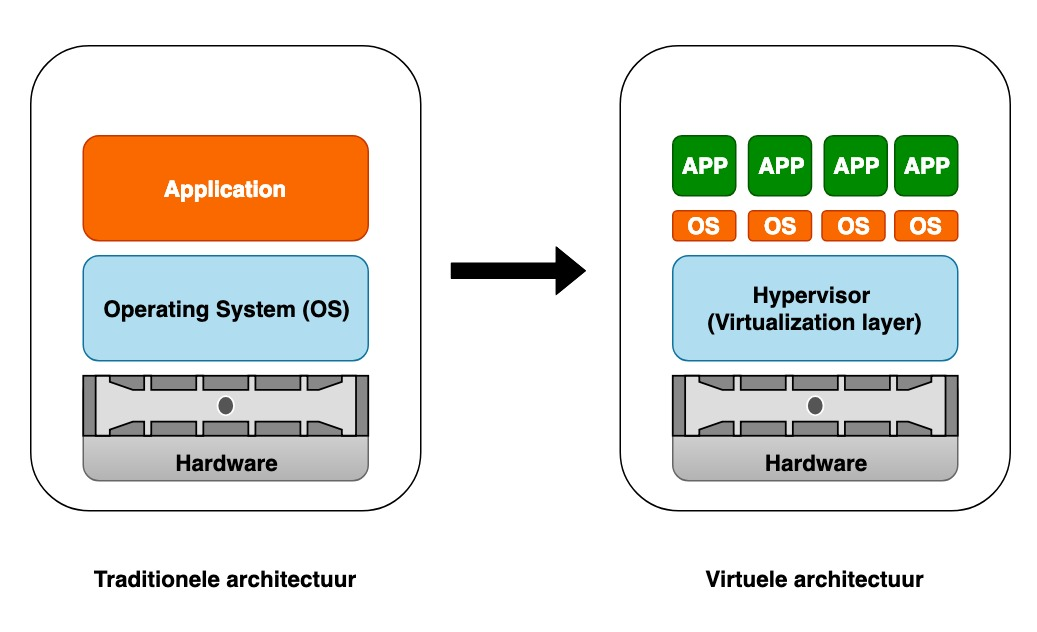
\includegraphics[width=1\textwidth]{img/klassiek_virtualisatie}
    \caption{De architectuur aan de linkerkant weergeeft een beeld van hoe de traditionele server architectuur eruit zag. De afbeelding rechts toont hoe een gevirtualiseerde architectuur eruitziet.} 
    \label{fig:klassiek-vs-virtualisatie}  
\end{figure}
\newline

Wanneer er naar de cloud gerefereerd wordt, dan bedoelt men meestal de cloud services die grote providers als een Google, Amazon en Microsoft aanbieden. Laten we de conventie maken dat wanneer er in de inleiding gerefereerd wordt naar de cloud, dat dit wijst op de cloud services die door cloud providers worden aangeboden. Later maken we de distinctie tussen welke verschillende soorten cloud er zijn met elk hun eigenschappen. De afgelopen jaren hebben steeds meer bedrijven gekozen om hun applicaties en infrastructuur naar de cloud te migreren. Migratie naar de cloud is interessant in verschillende opzichten, er zijn heel wat voordelen aan verbonden die in sectie ~\ref{voor-en-nadelen} worden uitgelegd. De grootste motivatie waarom bedrijven naar de cloud migreren is enerzijds het feit dat er enkel betaald wordt voor wat men verbruikt en anderzijds neemt het heel wat overhead zoals het onderhouden van infrastructuur weg. Cloud computing zorgt ervoor dat gebruikers een gedeelde poel van resources en opslag kunnen gebruiken bij een cloud provider, deze poel kan worden gezien als duizenden servers waarop virtuele machines of applicaties die worden aangeboden kunnen worden gedraaid. Deze services worden verschaft via het internet. Gebruikers betalen enkel voor de resources die ze verbruiken, zo worden de kosten meestal berekend op de tijd die een server draait en welke gespecificeerde resources deze verbruikt, zo een model wordt ook wel het ''Pay as you go model'' genoemd . De cloud is veelzijdig en biedt mogelijkheden op verschillende niveaus, deze worden in volgende onderdelen besproken.\autocite{Seghal2018} 


\subsection{Cloud types op deployment niveau}
\label{cloud-deployment-level}
De Cloud kan worden onderverdeeld in verschillende types op niveau van deployment. De onderverdeling op deployment level slaat op de locatie waar de cloud infrastructuur draait, bijvoorbeeld in een datacenter van een grote cloud provider of bij een bedrijf op locatie in een eigen datacenter. Volgens \textcite{Goyal2014} kan de cloud worden opgedeeld in vier verschillende soorten met elk hun specifieke eigenschappen. Om te beginnen wordt ook besproken wat men bedoelt met on-premises infrastructuur.

\subsubsection{On-premises}
Een on-premises infrastructuur wijst op een IT infrastructuur die wordt beheerd door een organisatie zelf, de apparaten bevinden zich ook op locatie bij het bedrijf. Een organisatie die over een on-premises of op locatie infrastructuur beschikt staat in voor het volledige beheer hiervan, dit gaat van fysieke installatie van apparaten netwerk enzovoort tot het beveiligen van applicatie op niveau van software. Een on-premises installatie zien we vaak terug in klassieke benaderingen of in bedrijven waar ze nog niet overtuigd van het hele cloud gebeuren. Sommige organisaties kiezen expliciet om hun infrastructuur niet in de cloud te draaien om allerhande redenen gerelateerd aan privacy en confidentialiteit van data.

\subsubsection{Publieke cloud}
De publieke Cloud wordt onderhouden door een derde partij. Publieke cloud providers bieden services en resources aan die op basis van een soort huurcontract aan externen worden verschaft. Klanten die services of infrastructuur huren bij publieke cloud providers kunnen deze raadplegen via het internet. Publieke cloud services worden verschaft aan iedereen, ze zijn met andere woorden voor iedereen toegankelijk. De publieke cloud stelt organisaties in staat te besparen op aankoop van infrastructuur. Het is mogelijk om te betalen naargelang de resources of diensten die worden gebruikt en dit is een heel interessant aspect van de publieke cloud. Data die gemaakt of opgeslagen wordt door gebruikers bevindt zich ook in het datacenter van de cloud provider. Voorbeelden van publieke cloud providers zijn, zoals eerder al aangehaald, Google, Amazon en Microsoft.

\subsubsection{Private cloud}
Private cloud bestaat in verschillende opzichten, het kan een datacenter zijn dat op locatie staat en onderhouden wordt of een cloud infrastructuur zijn die is opgezet in een datacenter waar servers worden gehuurd. Een private cloud wordt door de organisatie zelf volledig onderhouden, er is ook enkel toegang voor de organisatie zelf of voor toegestane derde partijen. Wanneer er gekozen wordt voor een private cloud infrastructuur dan brengt dit de veelzijdigheid en tools van cloud computing met zich mee, het is mogelijk dezelfde tools uit de publieke cloud op te zetten in een private cloudomgeving. Private cloud wordt vooral gekozen voor het waarborgen van privacy en veiligheid van data. Deze benadering wordt door veel bedrijven gekozen die veel confidentiële- en bedrijfskritische data moeten verwerken, denk maar aan banken, overheid en farmaceutica.

\subsubsection{Hybride cloud}
Een hybride cloud bestaat uit minstens één private en één publieke cloud. Wanneer verschillende soorten cloud met elkaar worden samengebracht wordt er verwezen naar een hybride cloud. Een hybride cloud wordt opgezet volgens verschillende standaarden en cloud- en apparatuur specifieke patenten. Een hybride cloud biedt de veelzijdigheid voor up- en down schaling zoals in de publieke cloud, en de veiligheid en integriteit zoals in de private cloud. Het implementeren van een hybride cloud omgeving is moeilijker omdat security hier heel wat overhead met zich meebrengt.

\subsubsection{Communtiy cloud}
Community cloud valt tussen de publieke en private cloud. Een community cloud bestaat uit twee of meer deelnemende partijen. Dit type van cloud valt te vergelijken met de private cloud die gedeeld wordt door meerdere partijen. Gebruik van een community cloud reduceert de aankoopkost van infrastructuur en de management kosten voor het opzetten van het cloud datacenter.


\subsection{Cloud service modellen}
\label{cloud-service-level}
Naast onderscheid op basis van de locatie waar cloud infrastructuur gedeployed wordt, maakt men ook onderscheid op niveau van service. Termen zoals PaaS, IaaS en SaaS horen tot deze sectie \autocite{Goyal2014}, in volgende drie secties worden deze veelvoorkomende klassieke cloud computing modellen samengevat.

\subsubsection{Infrastructure-as-a-Service (IaaS)}
Het IaaS service model biedt gebruikers computing, processing, networking en opslag aan waarop applicaties en dergelijke kunnen worden gedraaid. De gebruiker heeft de mogelijkheid om bovenop hardware die voorzien wordt door de cloud provider in te staan voor het volledige beheer van de infrastructuur. De componenten die aanpasbaar zijn, zijn onder andere het OS, de middleware, runtime, data en applicaties. De cloud provider staat in voor de networking, opslag, fysieke servers en bovenliggende virtualisatie. IaaS vormt de basis waarop Cloud computing is gebouwd, overige service modellen bouwen hierop ook verder. Gebruikers die controle willen hebben over (bijna) alle onderdelen van hun cloud infrastructuur opteren voor het gebruik van IaaS. Voorbeelden van IaaS zijn onder andere Google Cloud Platform Compute Engine, Amazon Web Services EC2 en Microsoft Azure.

\subsubsection{Platform-as-a-Service (PaaS)}
PaaS is vooral gericht op ontwikkelaars. Platform-as-a-Service stelt gebruikers in staat op een eenvoudige manier softwareapplicaties op te zetten zonder zorgen over de onderliggende infrastructuur. Cloud providers die PaaS diensten verschaffen staan in voor het volledige beheer van de infrastructuur zoals servers, zowel virtueel als fysiek, computing, opslag, netwerk, beveiliging, bijhorende tools en API's. Het beheer van servers zoals OS en dergelijke wordt ook door de cloud provider voorzien, PaaS voorziet een platform om applicaties op te draaien. Gebruikers staan enkel in voor ontwikkeling van de applicatie en de data die daar bijhoort. Als PaaS oplossing wordt vaak AWS Elastic Beanstalk gebruikt.

\subsubsection{Software-as-a-Service (SaaS)}
In het Software-as-a-Service model wordt de gehele infrastructuur inclusief applicatie beheerd door de provider. SaaS voorziet applicaties die draaien in de cloud en raadpleegbaar zijn via een computer of mobiel apparaat, vaak simpelweg via een webbrowser. In het verleden moest software meestal worden aangekocht en worden geïnstalleerd op individuelen systemen, SaaS is hiervoor de oplossing. Wanneer er gebruik wordt gemaakt van SaaS wordt de software aangerekend ob basis van subscripties per gebruiker, dit kan op basis van tijd of verbruik. SaaS draait, zoals eerder gezegd, in de cloud en vereist dus geen extra installatie van software. Eén van de bekendste SaaS applicaties is Office 365, deze Microsoft services werken met een maandelijkse subscriptie die betaald wordt per gebruiker. Een voorbeeld van een gratis SaaS applicatie is bijvoorbeeld Google Docs.
\begin{figure}
    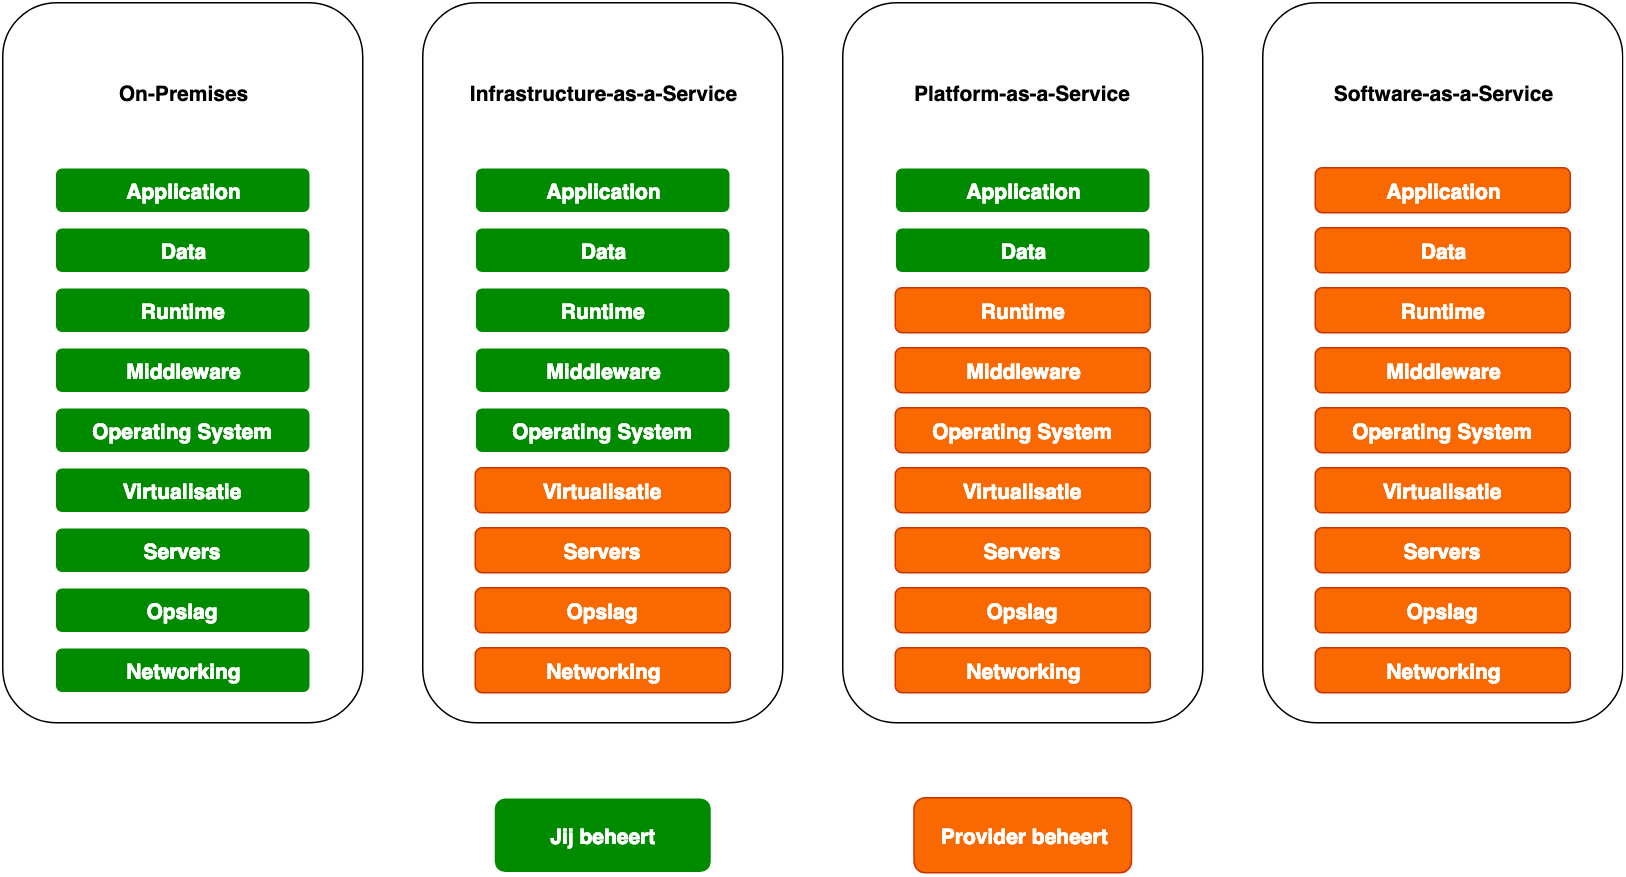
\includegraphics[width=1\textwidth]{img/cloud_service_level.png}
    \caption{De afbeelding weergeeft een schematische voorstelling van de verschillende cloud service niveaus. De groene kleur duidt alle onderdelen aan die zelf te managen zijn. De oranje kleur geeft aan welke onderdelen de cloud provider beheert.} 
    \label{fig:cloud-service-levels}  
\end{figure}
\newline

\subsection{Voor-en nadelen}
\label{voor-en-nadelen}
Cloud computing kent voordelen die heel wat mogelijkheden bieden ten opzichte van de klassieke benadering omtrent infrastructuur. \autocite{Azure2019} De voordelen zijn veelbelovend maar ook de nadelen mogen zeker niet over het hoofd worden gezien en dienen in kaart te worden gebracht om op de hoogte te zijn van mogelijke gevaren en bedreigingen.\autocite{Sosinsky2011} 

\subsubsection{Voordelen}

\begin{description}[style=unboxed, labelwidth=\linewidth, listparindent =0pt]
    \item[Lagere kosten]
    Cloud computing zorgt ervoor dat bedrijven zelf geen fysieke hardware meer hoeven aan te kopen voor hun eigen datacenter om software en applicaties te draaien. Een bedrijf hoeft bijvoorbeeld zelf geen webserver meer aan te kopen en te installeren om een webapplicatie te kunnen draaien, de benodigde hardware is beschikbaar bij verschillende cloud providers. Daarnaast zijn er ook geen kosten voor elektriciteitsvoorzieningen. De enige kost zijn de prijzen die de cloud provider aanrekent om de apparatuur of diensten ter beschikking te stellen.
    \newline

    \item[Performantie]
    Datacenters van grote cloud providers bevinden zich verspreid doorheen de hele wereld. De verspreiding van datacenters zorgt voor een lage latency en zorgt ervoor dat werken in de cloud voelt alsof de server in het eigen bedrijf staat. Computing componenten worden ook geregeld geüpgrade naar de laatste versies zodat de performantie verzekerd kan worden.
    \newline

    \item [Veiligheid]
    Doordat servers en opslag niet meer op locatie staan bij bedrijven wordt de kans op datadiefstal al sterk gereduceerd. Er is geen fysieke toegang meer tot infrastructuur en dus zal het onmogelijk zijn om via deze weg data te stelen. Daarnaast zijn datacenters uitgerust met dedicated beveiligingsapparatuur die in vele bedrijven niet aanwezig is. Datacenters zelf zijn erg goed beveiligd, het is haast onmogelijk deze gebouwen te betreden. Op softwareniveau bieden cloud providers ook heel wat diensten aan die helpen bij het beveiligen van applicaties.
    \newline

    \item [Schaalbaarheid en flexibiliteit]
    Cloud computing stelt in staat om up- en down te schalen volgens de noden. Dit wilt zeggen dat een bedrijf eender wanneer kan opteren om meer of minder middelen te huren naar gelang wat nodig is. Cloud computing is met andere woorden elastisch. Een bedrijf zoals Tomorrowland kan bijvoorbeeld doorheen het jaar, wanneer er geen ticketverkoop aan de gang is, de requests naar hun webservers bolwerken met 10 operationele servers. Indien er een ticketverkoop start kan het bedrijf kiezen om op te schalen naar 300 webservers zodat alle requests kunnen worden behandelt zonder dat dit veel moeite kost. De nood voor 30 keer meer servers is, wanneer deze manueel worden geïnstalleerd en opgezet op locatie, een taak die heel veel tijd en werk in beslag neemt maar die in de cloud zo is verwerkt. Dit voorbeeld toont aan dat de cloud mogelijkheden biedt om op een eenvoudige manier te schalen zonder dat dit handenvol geld kost (infrastructuur, tijd).
    \newline
  
\end{description}

\subsubsection{Nadelen}


\begin{description}[style=unboxed, labelwidth=\linewidth, listparindent =0pt]
        \item[Latency]
        Wanneer datacenters ver liggen vanwaar de servers worden geraadpleegd. Bijvoorbeeld je gebruikt thuis, in België, een applicatie die draait in een datacenter in de Verenigde staten, dan kan er latency optreden. Latency is vertraging in datacommunicatie tussen twee systemen, ook wel bekend als ''lag''. Dit probleem begint stilaan te verdwijnen aangezien alle grote cloud providers datacenters verdeeld hebben over de hele wereld.
        \newline
        
        \item[Privacy en security]
        Data legt meestal een langere weg af tussen een klant en cloud provider wanneer er gebruik wordt gemaakt van cloud services dan wanneer die klant zelf gebruik maakt van een infrastructuur op locatie. De langere route die de data neemt brengt ook meer gevaar met zich mee, hoe verder data moet reizen, hoe meer kans op onderschepping. Daarnaast is er vaak geen garantie of de overheid niet meekijkt naar de data die zich in datacenters bevindt bij publieke cloud providers. Datacenters zijn voor hackers ook grote doelwitten omdat ze met mogelijke inbraken hier veel mensen mee kunnen treffen en gegevens kunnen stelen.
        \newline
        
        \item [Vendor lock-in]
        Wanneer er gekozen wordt om gebruik te maken van diensten die een bepaalde cloud provider aanbiedt dan zit je vast aan die cloud provider en is overstappen met je hele infrastructuur vaak een zware klus. Kiezen om over te stappen naar een andere provider brengt mogelijks heel wat complexiteit en problemen met zich mee.
        \newline
        
        
        \item [Afhankelijk van netwerkconnectiviteit]
        Bij gebruik van de publieke cloud is er steeds afhankelijkheid van netwerkconnectiviteit. Wanneer een internetverbinding niet mogelijk is door eventuele problemen bij de Internet Service Provider (ISP) dan kan de cloud niet bereikt worden en zorgt dit voor grote problemen wanneer een bedrijf afhankelijk is van alles wat in de cloud draait. Daarnaast is het ook van belang dat er een snelle netwerkverbinding met voldoende bandbreedte beschikbaar is om effectief en efficiënt gebruik te maken van de cloud.
        \newline
        
        \item [Downtime]
        Downtime is een nadeel dat nog voor problemen kan zorgen. Wanneer een infrastructuur gedraaid wordt binnen een bepaald datacenter en dit gaat neer door interne problemen (technische problemen, onderhoud, gefaalde update/upgrade, brand, natuurramp, ...) dan zijn de infrastructuur en diensten (tijdelijk) niet meer bereikbaar. In het allerslechtste geval kunnen zo ook alle gegevens verloren raken wanneer er geen failover voorzien werd naar een ander datacenter (bijvoorbeeld in geval van een natuurramp). De kans dat dit voorkomt is echter nihil.
\end{description}
\newpage

\section{Wat is Serverless?}
Sinds de geboorte van de cloud hebben cloud diensten en technologieën een enorme (re)volutie gekend, denk maar aan de brede waaier van diensten die grote cloud providers vandaag aanbieden. Serverless  is ook een technologie die nog maar enkele jaren wordt aangeboden door cloud providers. Velen hebben waarschijnlijk wel al eens over de term ''Serverless'' gehoord maar weten vaak niet wat het inhoudt. Serverless wordt vaak omschreven als de volgende evolutie in cloud computing, een die van gelijkaardig succes kan zijn als het succes van zijn voorgangers zoals IaaS, PaaS en SaaS. Serverless brengt heel wat begrippen met zich mee, deze worden allemaal behandelt in volgende secties.
 
\subsection{Definitie}
De termen serverless en FaaS worden vaak door elkaar gebruikt en deze verwijzen dan vaak naar het volledige serverless plaatje, toch betekenen ze beiden niet hetzelfde. Wanneer er gesproken wordt over serverless computing dan kan er een onderscheid worden gemaakt in twee onderdelen met elk zijn eigen specifieke eigenschappen. Enerzijds is er Backend-as-a-Service (BaaS) en anderzijds Function-as-a-Service (FaaS). Het onderscheid dat wordt gemaakt tussen beiden duidt ook meteen dat serverless meer is dan enkel FaaS en dat de term serverless en FaaS daarom niet als synoniemen gebruikt zouden mogen worden. Echter in de praktijk wanneer men spreekt over serverless, dan bedoelt men meestal altijd de FaaS benadering. Het vervolg van dit onderzoek richt zich ook op Function-as-a-Service. De bijhorende proof-of-concept is ook gebaseerd op Faas.\autocite{Roberts2017}

\subsubsection{Backend-as-a-Service (BaaS)}
Backend-as-a-Service stelt ontwikkelaars in staat om gebruik te maken van kant en klare oplossingen zodat ze zelf geen server-side of backend componenten meer hoeven te managen. BaaS is een cloud service model dat verantwoordelijk is voor het volledige management van  de backend van een applicatie. Ontwikkelaars kunnen het beheer van backend servers outsourcen aan aanbieders van Backend-as-a-Service, dit stelt hun in staat te focussen op hetgeen dat er voor hen wel toe doet namelijk de applicatie code, de frontend. Waar het op neer komt is dat BaaS applicaties opsplitst in meerdere kleine onderdelen, deze opsplitsing zorgt ervoor dat verschillende ontwikkelaars gebruik kunnen maken van dezelfde delen software die reeds eerder zijn geschreven en worden aangeboden door een Backend-as-a-Service vendor. Wat dit betekend is dat ontwikkelaars dus gebruik kunnen maken van bestaande modules en deze implementeren in de backend van hun applicatie, denk bijvoorbeeld aan een database achterliggend aan een applicatie, integratie met sociale media of een module voor gebruikersauthenticatie zoals Auth0. BaaS providers zoals Google's Firebase biedt bijvoorbeeld een database aan die in de backend wordt onderhouden en aangeboden door de BaaS providers zonder dat de ontwikkelaar zich moet focussen op dit backend component. Daarnaast bieden BaaS providers nog een waaier van andere diensten aan om het leven van een ontwikkelaar zo aangenaam mogelijk te maken.
\\
De server-side mogelijkheden die de meeste Backend-as-a-Service providers aanbieden zijn:
\begin{itemize}
    \item Hosting van de applicatie, het beheer van de servers waarop de applicatie draait
    \item Opslag in de cloud voor content die gegenereerd wordt door gebruikers
    \item Management van een achterliggende databank
    \item Push notificaties
    \item Authenticatie voor gebruikers
    \item Beheer van updates
\end{itemize}
BaaS is vooral terug te vinden in de ontwikkeling van mobiele applicaties, er wordt ook vaak naar gerefereerd als Mobile-Backend-as-a-service (MBaaS). Backend-as-a-Service wordt gezien als serverless benadering omdat de ontwikkelaar enkel nog focust op de code die hij schrijft en niet op de servers waarop deze code draait. Serverless of zonder servers betekend dus niet dat er geen servers zijn, maar gewoon dat een ontwikkelaar zich er geen zorgen meer hoeft over te maken. BaaS brengt een groot nadeel met zich mee en dat is de vendor lock-in. Wanneer een ontwikkelaar kiest voor diensten bij een bepaalde vendor, dan is het moeilijk om in latere stadia weg te gaan bij die vendor.\autocite{Cloudflare2019} 

\subsubsection{Function as a Service (FaaS)}
Wanneer er gesproken wordt over serverless dan bedoelt men meestal de Function-as-a-Service cloud service en niet de Backend-as-a-Service benadering.  Function-as-a-Service is een trend in softwareontwikkeling die gebaseerd is op het schrijven en deployen van verschillende individuele functies.  
\\
In het deployment van klassieke applicaties wordt een applicatie traditioneel gedraaid in een virtuele machine (VM) of in een container. Wanneer de host een container of een VM is, dan draait de applicatie als proces bovenop op het besturingssysteem. De achterliggende code van een applicatie bevat vaak verschillende, aan elkaar gerelateerde, methoden met elk hun eigen functionaliteit.  Figuur \ref{fig:traditional-software-deployment} geeft een visualisatie van klassieke software deployment benadering, er is duidelijk te zien dat binnen een host de applicatie draait als een proces met daarbinnen de individuele methoden die elkaar aanspreken om de functionaliteit van de applicatie te garanderen.
\begin{figure}
    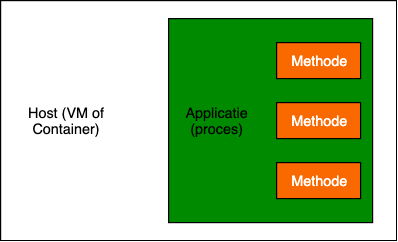
\includegraphics[width=0.7\textwidth]{img/traditional_software_deployment.png}
    \caption{Klassieke monoliet applicaties draaien als één proces op een besturingssysteem binnen een container of virtuele machine. Ee klassieke applicatie is opgebouwd uit verschillende methoden met elk hun eigen functionaliteit gescheiden door softwareklassen.} 
    \label{fig:traditional-software-deployment}  
\end{figure}
\\
De FaaS benadering verandert het klassieke model van applicatie deployment. Ontwikkelaars schrijven in dit model individuele functies die losstaan van elkaar en elk hun eigen specifieke taak hebben. Een applicatie draait nu niet meer voortdurend in een VM of container maar de functionaliteit werkt event-driven. De functies die de ontwikkelaar schrijf worden opgeladen naar een FaaS platform. Omdat de applicatie niet meer voortdurend draait is het FaaS platform zo geconfigureerd dat het luistert naar events die gekoppeld zijn aan een specifieke functie. Wanneer er een event optreedt dat een functie aanroept dan zorgt het FaaS platform ervoor dat er een container op wordt gebracht, de code wordt ingeladen en uitgevoerd en na afloop van de functie wordt de container weer gestopt. Functies worden vaak aangeroepen aan de hand van HTTP API Gateway calls, in de voorbeelden die volgen wordt de cyclus van FaaS duidelijk weergegeven. Hoe dit nu serverless is? Wel , ontwikkelaars dienen zich enkel maar te focussen op het schrijven van code (functies) en deze plaatsen ze gewoon in het FaaS platform, de achterliggende infrastructuur daar hoeven ze zich niets van aan te trekken.\autocite{Roberts2017}
\\\\
Er zijn al heel wat cloud providers die Function-as-a-Service platforms aanbieden en de populairste op moment van schrijven zijn ongetwijfeld: Amazon Web Services met hun AWS Lambda, Google Cloud Platform met Google Cloud Functions en Microsoft Azure met Azure Functions. De opgesomde platformen zijn allen proprietary en dus niet open-source. De FaaS platformen die de grote spelers aanbieden zijn al ver ontwikkeld en bieden heel wat functionaliteit maar zullen niet verder behandelt worden in dit onderzoek. Als alternatief duiken er steeds meer en meer open-source frameworks op voor het opzetten van een FaaS platform. In verder onderzoek zal een overweging worden gemaakt welke twee open-source frameworks het meest interessant zijn voor Nubera, die aan hun vereisten voldoen.

\section{Serverless concepten, begrippen en onderdelen}
Wat serverless nu precies voorstelt zou na het lezen van de definities al een stuk duidelijker moeten zijn. Serverless brengt echter nog meer begrippen mee om het volledige plaatje te kunnen schetsen. In deze sectie worden de belangrijkste ''key concepts'' uitgelegd.

\subsubsection{Next-Gen applicaties}
Naar applicaties die draaien in een serverless omgeving wordt vaak gerefereerd als next-gen applicaties. Met next-generation applicaties bedoelen we de applicaties die in een Cloud gebaseerde omgeving draaien en een onderliggende architectuur hebben die bestaat uit enerzijds containers en anderzijds microservices. Applicatieontwikkeling is de afgelopen jaren enorm veranderd, nu is het hele development gebeuren gericht op continue integratie en continue delivery (CI/CD) en zijn de ontwikkelingscyclussen (tijd tussen applicatie releases) verkleind van een aantal weken of aantal maanden tot een aantal minuten, uren of weken in het slechtste geval. 

\subsubsection{Microservices}
Microservices is een alternatief voor klassieke monoliet applicaties, dit zijn applicaties die verschillende functionaliteiten omvatten en draaien als een enkel proces binnen een VM of container. Een monoliet applicatie kan worden gezien als één gehele applicatie die draait op één machine.  In microservices daarentegen worden verschillende functionaliteiten en services gegroepeerd in groepen met elk hun eigen verantwoordelijkheden. Microservices zijn als het ware  een decompositie van een monoliet applicatie. Applicaties ontwikkeld volgens een microservices architectuur bestaan uit onafhankelijke componenten die naast elkaar bestaan en makkelijk vervangbaar of upgradebaar zijn. In een klassiek ontwerp van een applicatie is de applicatielogica van elkaar gescheiden door behulp van verschillende softwareklassen, deze kunnen met elkaar communiceren. In een microservice architectuur kunnen de verschillende componenten ook met elkaar communiceren maar dit gebeurt aan de hand van REST API vaak via het HTTP protocol. Daar waar monoliet applicaties gebruik maken van eenzelfde datastore, zijn elk component van microservices verantwoordelijk voor hun eigen data en persistentie. Een microservice kan de data van een andere microservice niet rechtstreeks raadplegen. Verschillende microservices kunnen draaien in verschillende VMs of containers, daarom wordt deze architectuur ook wel loosely-coupled genoemd.\autocite{Fowler2014}

\subsubsection{Containers}
Containers zijn te vergelijken met zeer kleine VMs 
\subsubsection{API Gateway}

\section{Serverless architectuur}


%%=============================================================================
%% Methodologie
%%=============================================================================

\chapter{Methodologie}
\label{ch:methodologie}

%% TODO: Hoe ben je te werk gegaan? Verdeel je onderzoek in grote fasen, en
%% licht in elke fase toe welke stappen je gevolgd hebt. Verantwoord waarom je
%% op deze manier te werk gegaan bent. Je moet kunnen aantonen dat je de best
%% mogelijke manier toegepast hebt om een antwoord te vinden op de
%% onderzoeksvraag.

\section{Voorbereiding}
Als eerste heb ik mij de eerste weken van het tweede semester verdiept in het onderwerp, vooral door YouTube video's te kijken maar ook door artikels en blogs te lezen. Ik heb mij ook  verdiept in cloud computing aan de hand van een course op Pluralsight waarin de basisconcepten van cloud computing werden uitgelegd. Ik had nog niet echt kennis van cloud computing en totaal geen kennis van serverless dus geregeld hier wat rond lezen of bekijken hielp mij wel om een beter beeld te krijgen van het volledige plaatje. 

\section{Stand van zaken}
Vervolgens ben ik gestart met het schrijven van mijn literatuurstudie. In de literatuurstudie start ik met een uiteenzetting van cloud computing concepten en principes om vervolgens verder te gaan op serverless. Het volledige serverless plaatje wordt behandeld en gecapteerd aan de hand van duidelijke voorbeelden met afbeeldingen die verschillende componenten visueel voorstellen. De literatuurstudie is geschreven op basis van boeken omtrent cloud computing en serverless infrastructuur. Vanuit wetenschappelijke artikels werden juiste feiten gehaald om vervolgens zo nauwkeurig mogelijke artikels, conferenties en documentatie te verzamelen die inzicht geven in het onderwerp.

\section{Uitwerking}
Bij het schrijven van hoofdstuk \ref{ch:uitwerking} wordt de zoektocht naar 
 serverless frameworks, die in aanmerking komen voor deze bachelorproef, beschreven. Het hoofdstuk vat aan met een inleiding waarin wordt uitgelegd waarnaar er op zoek wordt gegaan. De zoektocht naar mogelijke open source frameworks is vertrokken vanuit een requirements analyse waarin alle requirements opgelegd door Nubera in vermeld staan. Op basis van enkele requirements werden frameworks die in aanmerking komen gekozen. Vervolgens werden de frameworks aan de hand van de requirements ten opzichte van elkaar vergeleken en werd er een lijst opgemaakt waarin de meest veelbelovende frameworks werden gerangschikt van boven naar onder. Op basis van de rangschikking werd het meest veelbelovende framework gekozen samen met Fission, dit was reeds vastgelegd door Nubera. Het gekozen framework en Fission vormen samen de short list. In de short list werd verder onderzoek gedaan naar de frameworks, wat ze inhouden en hoe de architectuur ervan eruitziet. Na de zoektocht worden beide frameworks opgezet in een Proof of Concept om deze tegenover elkaar af te wegen.

\section{Proof of Concept}

\chapter{Uitwerking}
\label{ch:uitwerking}

Dit hoofdstuk bevat het onderzoek naar open source tools die in aanmerking komen als alternatief voor Fission. Er worden requirements vastgelegd in overleg met Nubera, op basis van deze requirements wordt een long list opgesteld met tools die in aanmerking kunnen komen. Na het evalueren van de long list worden de frameworks beoordeeld volgens het aantal requirements waaraan voldaan werd, het meest interssante framework vormt samen met Fission de shortlist.

\section{Open Source tools}
Het onderwerp van deze bachelorproef gaat over een vergelijking tussen open source serverless frameworks voor het draaien van een serverless infrastructuur in house, dit betekent concreet binnen het hele bedrijf. In house duidt op alle infrastructuur waar een organisatie gebruik van maakt, on-premises infrastructuur zoals een eigen datacenter maar ook private cloud behoren hiertoe. Het is van belang om nog even te vermelden dat deze bachelorproef zich focust op het FaaS model en niet op het BaaS model. Nubera biedt momenteel nog geen vast serverless (FaaS) framework aan bij klanten, voor hun is dit onderzoek zinvol zodat iedereen binnen Nubera een beeld heeft over wat serverless precies is en hoe dit kan worden opgezet. Nbubera experimenteert reeds met Fission en wilt zoekt een alternatief framework hiervoor. De requirements waaraan de frameworks moeten voldoen worden opgelijst in volgende sectie. De opzet van deze studie maakt een vergelijking tussen twee open source frameworks die ik op basis van enkele requirements vergelijk. Het eerste framework waar Nubera interesse in heeft is Fission, dit zal uitgewerkt worden aan de hand van een Proof of Concept. Een tweede framework dat fungeert als vergelijking, wordt gekozen aan de hand van de requirements die werden vastgelegd.

\section{Requirements analyse}
Hier worden de requirements waaraan de open source frameworks moeten voldoen opgelijst, zowel functionele als niet-functionele. De requirements worden vervolgens onderverdeeld in verschillende categorieën volgens prioriteit. De requirements werden gecapteerd in overleg met Nubera.

\subsection{Functionele requirements}
\subsubsection{Must-have}
\begin{itemize}
    \item Kubernetes als onderliggende laag.
    \item Ondersteund serverless functies in Python en GO.
    \item Auto-scalable.
    \item Snelle uitvoeringstijd van functies: In de Proof of Concept zal de uitvoeringstijd van dezelfde functie die wordt uitgevoerd op beide frameworks worden gemeten. Op basis van de resultaten worden conclusies getrokken.
\end{itemize}
\subsubsection{Should-have}
\begin{itemize}
    \item User interface voor makkelijk beheer van functies en API gateways.
    \item Ondersteund serverless functies in Node.js.
    \item YAML format voor templating en definiëring van functies.
\end{itemize}
\subsubsection{Nice-to-have}
\begin{itemize}
    \item Ondersteund serverless functies in nog meer verschillende talen zodat hetzelfde framework kan gebruikt worden bij verschillende klanten.
\end{itemize}
\subsection{Niet-functionele requirements}
\subsubsection{Must-have}
\begin{itemize}
    \item Het moet open source zijn.
    \item Het framework moet gratis zijn.
    \item Minstens 40 contributors op GitHub.
    \item Minstens 3000 stars op GitHub. (Garantie voor populariteit in de community.)
    \item Gebruiksvriendelijk: De eigen ervaring wordt hier als norm genomen, op basis van het uitproberen en experimenteren wordt deze requirement gemeten.
    \item Eenvoudig op te zetten: Het installatieproces van het framework is goed gedocumenteerd en is eenvoudig te reproduceren.
\end{itemize}
\subsubsection{Should-have}
\begin{itemize}
    \item Enige maturiteit als garantie voor het functioneren van het framework. (Production ready)
    \item Contributors uit erkende organisaties.
    \item Het project wordt onderhouden, laatste commit is niet ouder dan 2 weken. (Datum van schrijven 13/04/2019)
    \item Goede en duidelijke documentatie.
\end{itemize}
\subsubsection{Nice-to-have}
\begin{itemize}
    \item Slack channel over het project.
\end{itemize}

\section{Long list}
In deze sectie worden alle mogelijke frameworks die in aanmerking komen overeenstemmend met de gecapteerde requirements opgelijst. Per alternatief wordt de website vermeld volgens APA stijl er wordt ook een korte beschrijving gegeven. Na de oplijsting van de verschillende frameworks die in aanmerking komen worden er tabellen opgemaakt waarin terug te vinden is of de frameworks al dan niet aan de requirements voldoen, er is één tabel voor de functionele en één voor de niet-functionele requirements. Op basis van de tabellen worden drie frameworks (inclusief Fission) gekozen die verder worden verwerkt in de short list. De functionele en niet-functionele requirements worden per framework tegen elkaar afgewogen, executietijd van functies, gebruiksvriendelijkheid en eenvoud in installatie zijn niet meetbaar zonder Proof of Concept en zullen maar later in dit onderzoek worden gemeten. Deze requirements worden daarom ook niet in de tabellen opgenomen.

\subsection{Fission}
Fission\footnote{https://fission.io/} werd reeds vastgelegd door Nubera en is een Kubernetes native serverless framework voor functies. Het stelt ontwikkelaars in staat functies te schrijven, die een korte levensduur hebben, in verschillende talen. De functies kunnen worden gemapt aan HTTP triggers.

\subsection{Kubeless}
Kubeless\footnote{https://kubeless.io/} beschrijft zichzelf als een Kubernetes native serverless framework dat ontwikkelaars in staat stelt kleine stukken code of functies op te laden zonder zorg over de onderliggende infrastructuur. Kubeless is de ideale tool voor ieder die op zoek is naar een open source alternatief voor wat AWS Lambda, Google Cloud Functions en Azure Functions aanbieden.

\subsection{OpenFaaS}
\textcite{OpenFaaS2019} beschrijft zichzelf ook als een framework voor het bouwen van serverless functies met Kubernetes en Docker, het voorziet ook support voor metrics. Tools als Prometheus kunnen makkelijk worden geïmplementeerd voor monitoring.

\subsection{Apache OpenWhisk}
OpenWhisk\footnote{https://openwhisk.apache.org/} is een open source serverless platform dat als respons op events en triggers functies uitvoert. OpenWhisk staat in voor het beheer van de hardware en schaalbaarheid van applicaties met behulp van Docker containers zodat ontwikkelaars zich kunnen focussen op het bouwen van applicaties.

\subsection{Fn}
De beschrijving waarmee \textcite{FnProject2019} zichzelf voorstelt luidt als volgt: Het Fn Project is een open source container-native serverless platform dat overal kan draaien, in elk type van cloud maar ook op locatie. Het is makkelijk in gebruik, ondersteund elke programmeertaal, is uitbreidbaar en performant. 

\subsection{IronFunctions}
Iron belooft met hun IronFunctions\footnote{https://open.iron.io/} serverless framework dat taken die veel CPU vragen onmerkbaar in de achtergrond draaien. Het laat ontwikkelaars toe functies te implementeren in applicaties en de focus te leggen op het schrijven van de software. Het voorziet ook snelle en eenvoudige configuratie van de onderliggende infrastructuur en job processing.

\subsection{OpenLambda}
OpenLambda\footnote{https://open-lambda.org/index.htm} is in tegenstelling tot de eerder besproken alternatieven minder ver ontwikkeld. OpenLambda is een framework dat interessant is voor iedereen die wil wil testen en serverless wilt leren kennen. OpenLambda is niet production ready, de eerder besproken tools zijn dit vaak wel al.

\subsection{Nuclio}
Nuclio\footnote{https://nuclio.io} wordt vaak gebruikt als alternatief voor AWS Lambda. Nuclio is een serverless framework voor functies in real-time en data gedreven applicaties. Nuclio ondersteund ook Kubernetes als platform. \autocite{Nuclio2019}

\subsection{Knative}
Pivotal beschrijft Knative\footnote{https://pivotal.io/knative} als een uitbreiding van Kubernetes die helpt bij het bouwen van moderne, container-gebaseerde applicaties. Knative voorziet een eenvoudige manier voor ontwikkelaars om applicaties bovenop Kubernetes te draaien. Knative is een open source project in samenwerking met Google.

%bla bla in tabel x en in y worden vergeleken op basis van FR en NFR..
\subsection{Vergelijking}
In tabel \ref{frameworks-fr} worden de verschillende frameworks vergeleken op basis van hun functionele requirements die vooropgesteld  werden.  De tabel duidt de requirements waaraan de frameworks voldoen aan met een ''X'', indien ze niet voldoen volgt er een ''-'' of aangepaste omschrijving. Tabel \ref{frameworks-nfr} geeft een overzicht van de frameworks ten opzichte van de vooropgestelde niet-functionele requirements. In deze tabel geldt hetzelfde: een ''X'' wilt zeggen dat er aan de requirement is voldaan, een ''-'' betekent dat er een requirement niet voldaan is en een aangepaste beschrijving werd gekozen wanneer deze meer zegt dan een ''X'' of ''-''.

\begin{table}[]
    % \centering
    \resizebox{\textwidth}{!}{%
        \begin{tabular}{@{}llccccccccc@{}}
            \toprule
            \multicolumn{2}{l}{} & \textbf{Fission} & \textbf{Kubeless} & \textbf{OpenFaaS} & \textbf{OpenWhisk} & \textbf{Fn} & \textbf{IronFunctions} & \textbf{OpenLambda} & \textbf{Knative} & \textbf{Nuclio} \\ \midrule
            \multirow{3}{*}{\textbf{Must-have}} & Native Kubernetes & X & X & X & X & X & X & X & X & X \\
            & Python/GO support & X & X & X & X & X & X & Enkel Python & X & X \\
            & Auto-scalable & X & X & X & X & X & - & - & X & X \\
            \hline
            \multirow{3}{*}{\textbf{Should-have}} & User-interface & X & X & X & - & X & X & - & - & X \\
            & Node.js support & X & X & X & X & X & X & - & X & X \\
            & YAML templating & X & X & X & X & X & - & - & X & X \\
            \hline
            \textbf{Nice-to-have} & Support voor meer talen & X & X & X & X & X & X & - & X & X \\ \bottomrule
        \end{tabular}%
    }
    \caption{Vergelijking serverless frameworks op basis van functionele requirements}
    \label{frameworks-fr}
\end{table}


\begin{table}[]
    \resizebox{\textwidth}{!}{%
        \begin{tabular}{@{}llccccccccc@{}}
            \toprule
            &  & \textbf{Fission} & \textbf{Kubeless} & \textbf{OpenFaaS} & \textbf{OpenWhisk} & \textbf{Fn} & \textbf{IronFunctions} & \textbf{OpenLambda} & \textbf{Knative} & \textbf{Nuclio} \\ \midrule
            \multirow{4}{*}{\textbf{Must-have}} & Open source & X & X & X & X & X & X & X & X & X \\
            & Gratis & X & X & X & X & X & X & X & X & X \\
            & > 40 contributors & 76 & 77 & 99 & 151 & 77 & 32 & 17 & 115 & 36 \\
            & > 3K GitHub stars & 4.2K & 4.5K & 13.8K & 3.9K & 3.9K & 2.5K & 593 & 1.6K & 2.6K \\
            \hline
            \multirow{4}{*}{\textbf{Should-have}} & Maturiteit (Production ready) & X & X & X & X & X & - & - & X & X \\
            & Mede ontwikkeld door erkende organisaties & Platform9 & Bitnami & VMWare & IBM & Oracle & iron.io & - & Google & - \\
            & Laatste commit (datum schrijven 13/04/2019) & 09/04/2019 & 09/04/2019 & 13/04/2019 & 11/04/2019 & 10/04/2019 & 20/08/2018 & 14/01/2019 & 13/03/2019 & 01/04/2019 \\
            & Goede/duidelijke documentatie & X & X & X & X & - & - & - & X & X \\
            \hline
            \textbf{Nice-to-have} & Slack channel over het project & X & X & X & X & X & - & - & X & X \\ \bottomrule
        \end{tabular}%
    }
    \caption{Vergelijking serverless frameworks op basis van niet-functionele requirements}
    \label{frameworks-nfr}
\end{table}

\subsubsection{Resultatenverwerking}
Eerst worden de functionele requirements behandeld. Op basis van tabel \ref{frameworks-fr} is onmiddellijk zichtbaar dat enkele frameworks minder interessant zijn dan anderen. IronFunctions en OpenLambda voldoen niet aan de must-have requirements en worden dus niet verder behandeld. OpenWhisk en Knative worden niet geleverd met een user interface en voldoen zo beiden niet aan de should-have functionele requirements. Alle overige kandidaten voldoen aan de nice-to-have requirements, namelijk ondersteuning voor meerdere programmeertalen.
\\\\
Vervolgens worden de niet-functionele requirements bekeken. De tabel weergeeft dat alle frameworks open source en gratis zijn, deze requirements worden dus voor alle frameworks voldaan. De volgende requirements die in acht worden genomen zijn het aantal contributors eveneens als het aantal ''stars'' op GitHub. Een hoger aantal contributors wijst vaak op meer kennis, meer review van code en enige zekerheid in vergelijking met een laag aantal contributors. De GitHub stars worden als factor gekozen om te meten hoe populair een framework is. De metingen werden gedaan op 13 april 2019 en kunnen tegen de tijd van lezen reeds gewijzigd zijn. Als norm werd vooropgesteld dat een project minstens veertig contributors moet hebben alsook een minimum van drieduizend stars. IronFunctions, OpenLambda en Nuclio voldoen niet aan het opgelegde aantal contributors. Knative, OpenLambda, Nuclio en IronFunctions behalen ook niet het minimum van drieduizend stars. Daarnaast worden ook de should-have requirements bekeken. Alle kandidaat frameworks voldoen aan maturiteit en zijn ''production ready''. Elk framework behalve Nuclio en OpenLambda wordt mede ontwikkeld door erkende organisaties, de bedrijven die werden opgelijst worden ook wel de ''backers'' van het project genoemd. Omdat Nuclio en OpenLambda geen erkende organisatie achter zich hebben worden deze kandidaten niet meer in overweging genomen. De datum van de laatste commit is ook een belangrijk gegeven om te beslissen of het project overlevingskans heeft en up-to-date blijft. Bij Knative dateert de laatste commit van een maand geleden wat erg lang is voor een open source project, ook deze optie wordt geschrapt. De overige kandidaten beschikken allemaal over een duidelijke documentatiewebsite, videobronnen en Slack channels om over het project te praten. Tabel \ref{frameworks-samenvattingl} weergeeft een samenvatting van de frameworks en het aantal requirements waaraan ze voldoen, ze worden gerangschikt volgens de graad dat ze in aanmerking komen, van boven naar beneden. In de tabel wordt telkens voor de verschillende categorieën van requirements een optelling gemaakt waaraan een framework voldoet. Uit de tabel is af te leiden dat OpenFaaS, Kubeless en Fission een maximumscore behalen. Na verder onderzoek werd besloten om verder te gaan met OpenFaaS als alternatief framework voor Fission. In sectie \ref{sec:short-list} worden Fission en OpenFaaS verder in detail besproken. Nubera gaf aan dat zij Fission een interessant framework vinden, dit zal worden opgezet in een Proof of Concept, daarnaast wordt als alternatief OpenFaaS opgezet als vergelijking. Aan de hand van de uitwerking moet blijken of Fission een goede keuze is of dat een ander alternatief misschien nog meer mogelijkheden biedt.
\\
\begin{table}[]
    \centering
    \resizebox{\textwidth}{!}{%
        \begin{tabular}{@{}llccccccccc@{}}
            \toprule
            &  & \multicolumn{3}{c}{\textbf{Functionele requirements}} & \textbf{} & \multicolumn{3}{c}{\textbf{Niet-functionele requirements}} & \textbf{} & \textbf{Totaal} \\ \midrule
            &  & \textbf{M-H} & \textbf{S-H} & \textbf{N-T-H} & \textbf{} & \textbf{M-H} & \textbf{S-H} & \textbf{N-T-H} & \textbf{} & \textbf{/16} \\
            \textbf{1.} & \textbf{OpenFaaS} & 3 & 3 & 1 &  & 4 & 4 & 1 &  & 16 \\
            \textbf{2.} & \textbf{Kubeless} & 3 & 3 & 1 &  & 4 & 4 & 1 &  & 16 \\
            \textbf{3.} & \textbf{Fission} & 3 & 3 & 1 &  & 4 & 4 & 1 &  & 16 \\
            \textbf{4.} & \textbf{OpenWhisk} & 3 & 2 & 1 &  & 4 & 4 & 1 &  & 15 \\
            \textbf{5.} & \textbf{Fn} & 3 & 3 & 1 &  & 4 & 3 & 1 &  & 15 \\
            \textbf{6.} & \textbf{Knative} & 3 & 2 & 1 &  & 3 & 4 & 1 &  & 14 \\
            \textbf{7.} & \textbf{Nuclio} & 3 & 3 & 1 &  & 2 & 3 & 1 &  & 13 \\
            \textbf{8.} & \textbf{IronFunctions} & 2 & 2 & 1 &  & 2 & 1 & 0 &  & 8 \\
            \textbf{9.} & \textbf{OpenLambda} & 1 & 0 & 0 &  & 2 & 0 & 0 &  & 3 \\
            &  & \multicolumn{1}{l}{} & \multicolumn{1}{l}{} & \multicolumn{1}{l}{} & \multicolumn{1}{l}{} & \multicolumn{1}{l}{} & \multicolumn{1}{l}{} & \multicolumn{1}{l}{} & \multicolumn{1}{l}{} & \multicolumn{1}{l}{} \\
            &  & \multicolumn{1}{l}{} & \multicolumn{1}{l}{} & \multicolumn{1}{l}{} & \multicolumn{1}{l}{} & \multicolumn{1}{l}{} & \multicolumn{1}{l}{} & \multicolumn{1}{l}{} & \multicolumn{1}{l}{} & \multicolumn{1}{l}{} \\ \bottomrule
        \end{tabular}%
    }
    \caption{Frameworks opgelijst in graad waarin ze in aanmerking komen. (M-H: Must-have, S-H: Should-have, N-T-H: Nice to have.) }
    \label{frameworks-samenvattingl}
\end{table}

\section{Short List}
\label{sec:short-list}

In deze sectie wordt op basis van voorgaande long list, zoals eerder al aangehaald, Fission en OpenFaaS vergeleken. Nubera wilt zeker verdere informatie en Proof of Concept over Fission, daarnaast willen ze ook een evenwaardig alternatief zodat op basis van dit onderzoek een keuze kan worden gemaakt. De verdere uitwerking tracht ook de requirments die nog niet werden gemeten te behandelen. De functionele requirement: Zo snel mogelijke uitvoeringstijd van functies en de niet-functionele requirements: gebruiksvriendelijk en eenvoudig op te zetten worden in de Proof of Concept verder onderzocht. 

\subsection{OpenFaaS}
OpenFaaS\footnote{https://www.openfaas.com/} is een open source Function as a Service (serverless) project dat werd opgestart door Alex Ellis. Alex is lid van het VMWare Open Source Technology Center (OSTC), VMWare is eveneens ''backer'' van dit project, ze ondersteunen in de ontwikkeling van OpenFaaS. Het project telt 13.8K GitHub stars, 99 contributors en is daarmee momenteel het grootste en populairste open source Function as a Service framework. OpenFaaS wordt al gebruikt bij verschillende grote organisaties zoals: VMWare, BT (British Telecom), Citrix, Contiamo, University of Washington, ... 
\\
De aspecten waarmee OpenFaaS uitpakt om zich te onderscheiden van anderen zijn: \autocite{OpenFaaS2019}
\begin{itemize}
    \item Makkelijke installatie en eenvoud in gebruik door de beschikbare UI.
    \item Portable: draait op bestaande hardware of in de public/private cloud maar ook op Kubernetes of Docker Swarm.
    \item Functies in eender welke taal voor Linux of Windows.
    \item Auto-scalable wanneer de vraag verhoogt.
    \item YAML format voor templating en definiëren van functies.
\end{itemize}
\subsubsection{Architectuur}
OpenFaaS kan worden opgedeeld in verschillende onderdelen met elk hun eigen verantwoordelijkheden.
\begin{figure}
    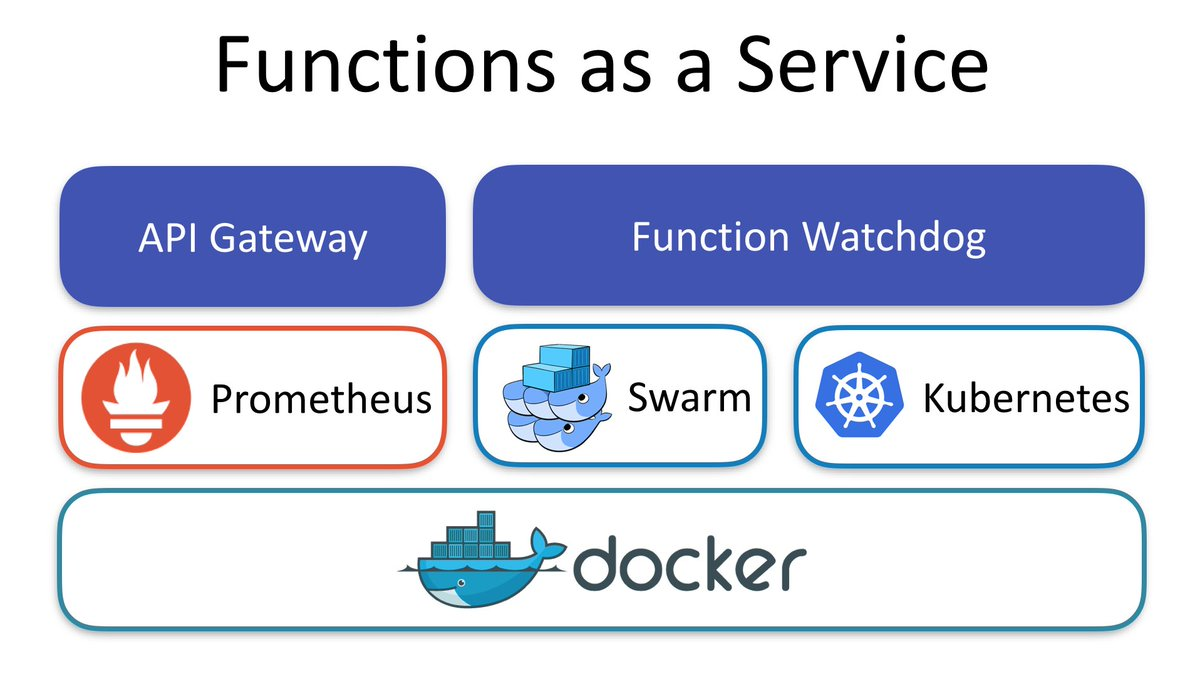
\includegraphics[width=1\textwidth]{img/open-faas.jpg}
    \caption{De figuur weergeeft een conceptuele voorstelling van de componenten van OpenFaaS. \autocite{Ellis2019}}
    \label{fig:open-faas-conceptueel}  
\end{figure}

\begin{description}[style=unboxed, labelwidth=\linewidth, listparindent =0pt]
    \item[Docker laag]
    In figuur \ref{fig:open-faas-conceptueel} is de onderste laag een volledige Docker laag, dit weergeeft dat alle functies die geschreven worden, worden uitgevoerd in Docker containers, deze containers bevatten alle dependencies nodig voor de code om uit te voeren.
    \newline
    
    \item[Swarm/Kubernetes]
    Bovenop de Docker laag in figuur \ref{fig:open-faas-conceptueel} is er een Swarm of Kubernetes component terug te vinden. Deze laag is de zogenoemde ''orchestrator'', deze staat in voor het management, configuratie en de coördinatie van de Docker containers.
    \newline
    
    \item[Prometheus]
    OpenFaaS maakt gebruik van Prometheus\footnote{https://prometheus.io/}, dit is een open source tool die instaat voor systeem monitoring en alerting. Prometheus verzamelt gegevens over de functies die kunnen worden weergegeven in een UI, namelijk Grafana dashboard.
    \newline
    
    \item[Function Watchdog]
    In figuur \ref{fig:open-faas-conceptueel} staat de Function Watchdog bovenop de reeds opgesomde componenten. Function Watchdog zorgt ervoor dat een Docker image kan worden omgevormd in een serverless functie, dit door het toevoegen van een kleine HTTP server. Daarnaast is de Function Watchdog eveneens het ingangspunt dat HTTP requests toelaat om geforward te worden naar het bestemmingsproces via HTTP of STDIN. Het responsbericht wordt teruggestuurd naar STDOUT of HTTP van de applicatie. \autocite{Ellis2019}
    \newline
    
    \item[API Gateway/UI Portal]
    De API Gateway in figuur \ref{fig:open-faas-conceptueel} verzorgt een route naar de geschreven functies, hier worden functies gedefinieerd, en verzameld metrics aan de hand van Prometheus. De API Gateway zorgt eveneens voor schaalbaarheid van functies door de vraag op te halen via de replica count in Docker Swarm of de Kubernetes API. Bij installatie van OpenFaaS wordt er ook een UI meegeleverd, deze laat gebruikers toe functies op te vragen en toe te voegen via deze interface. \autocite{Ellis2019} 
    \newline
    
    \item[CLI]
    Elk proces binnen een container of de container op zich kan een serverless functie zijn. OpenFaaS voorziet FaaS CLI om snel functies te deployen. Nieuwe functies kunnen worden gemaakt aan de hand van templates maar ook via een Dockerfile. \autocite{Ellis2019}  
\end{description}

\subsection{Fission}
Fission\footnote{https://fission.io} is een framework voor serverless functies op Kubernetes dat werd aangegeven door Nubera zelf, na verder onderzoek bleek dit ook te voldoen aan alle opgestelde requirements. Fission bestaat sinds augustus 2016 en wordt ontwikkeld en onderhouden door medewerkers van Platform9. Momenteel Heeft Fission 4K stars op GitHub en 76 contributors. Gebruikers die Fission reeds in hun organisatie implementeren zijn eveneens een stuk moeilijker te vinden in vergelijking met OpenFaaS.
\\
De  belangrijkste aspecten van Fission zijn:
\begin{itemize}
    \item Native Kubernetes: Fission draait op elke locatie op Kubernetes.
    \item Snelle cold-start: functies hebben een korte cold-start latency, lager dan ~100ms.
    \item Functie samenstelling: Fission Workflows zorgt ervoor dat ontwikkelaars niet moeten bezig zijn met networking, bericht wachtrijen of andere onderdelen die serverless functies complex maken.
    \item Administratie en operationele eenvoud: logs worden onmiddellijk via de CLI weergegeven daarnaast is er ook integratie met Prometheus voor het evalueren van metrics aan de hand van een duidelijk dashboard.
    \item Istio integratie: Fission integreert met Istio, een platform dat instaat voor management en beveiliging van microservices. Via dashboards kunnen gebruikers ook informatie ophalen over de latency van functies die worden aangeroepen.
    \item Declaratie van functies moet maar éénmaal door de ontwikkelaar worden gedaan, vervolgens kan de functie overal worden gedeployed.
    \item Ondersteuning voor meerdere programmeertalen: Python, Node.js, GO, C\#, PHP daarnaast kunnen ook eigen containers worden gebouwd indien dit nodig is. 
    \item Auto-scaling van functies. 
\end{itemize}

\subsubsection{Architectuur}
Fission bestaat uit verschillende componenten, met elk hun eigen verantwoordelijkheden. Hieronder wordt een overzicht gegeven hoe een Fission architectuur precies in elkaar zit. 

\begin{figure}
    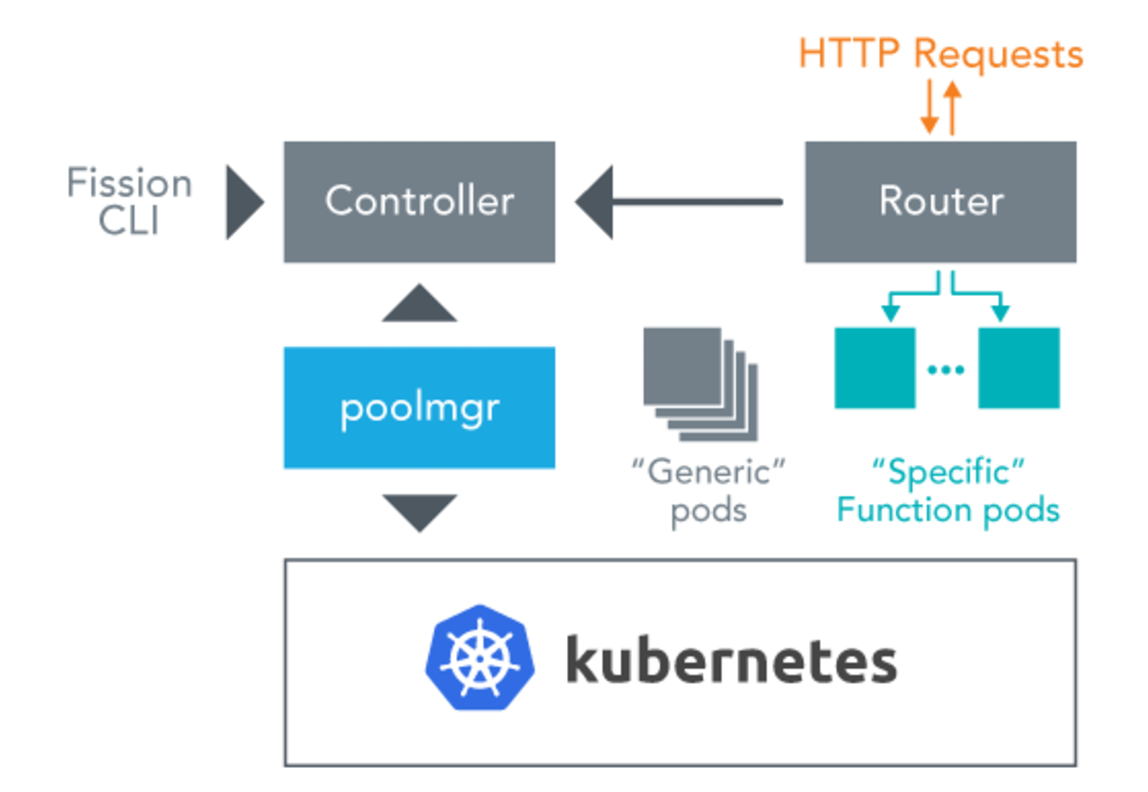
\includegraphics[width=1\textwidth]{img/fission_architectuur.png}
    \caption{Architectuur van een Fission infrastructuur die draait op een Kubernetes cluster. \autocite{Chemitiganti2018}}
    \label{fig:fission-architectuur}
\end{figure}

\begin{enumerate}
    \item Fission bestaat uit verschillende microservices. De controller houdt functies, event triggers, HTTP routes en omgevings images bij. Een pool manager (poolmgr) staat in voor het beheer van een groep omgevingscontainers (environment containers) die niet aan het draaien zijn. Daarnaast is de poolmgr ook verantwoordelijk voor het inladen van de functies in deze containers en na afloop de containers ook weer af te zetten. De router ontvangt, zoals te zien is in figuur \ref{fig:fission-architectuur} HTTP requests en routeert deze naar draaiende containers die de corresponderende functie bevatten, indien de nodige functie niet beschikbaar is wordt deze via de pool manager aangevraagd. \autocite{Chemitiganti2018}
    \item De controller bedient de Fission API terwijl alle andere componenten de controller in het oog houden voor updates. De router component wordt geëxposed als een Kubernetes dienst van de load balancer of NodePort type, dit afhankelijk van de locatie waar de cluster wordt gehost. Wanneer de router een HTTP request ontvangt kijkt hij eerst of er in de cache reeds een service is die gelinkt is met de request, zo niet zoekt hij de overeenstemmende functie om de request mee te mappen en vraagt hij de poolmgr voor een instantie. De poolmgr beschikt over een pool van pods die momenteel niet aan het werk zijn, de poolmgr kiest een pod waarin de functie wordt ingeladen. Als de functie is ingeladen wordt het adres van die pod teruggestuurd naar de router. De pod wordt nu opgeslagen in de cache voor toekomstige requests, indien er binnen enkele minuten geen nieuwe requests volgen wordt de pod gestopt.  \autocite{Chemitiganti2018}
    \item Fission voorziet een eenvoudige manier van functie deployment op alle Kubernetes clusters. Functies worden uitgevoerd los van elkaar.
    \item Voor het maken van complexere serverless applicaties moeten functies met elkaar kunnen communiceren en van elkaar gebruikmaken. Dit proces is vaak moeilijk en neemt veel tijd in beslag. Fission Workflows voorziet makkelijke orkestratie van een sequentie serverless functies voor het maken van een applicatie. \autocite{Chemitiganti2018}
    \item Workflows voorziet een makkelijke manier om serverless functies op elkaar af te stemmen en samen te laten werken aan de hand van sequenties van taken, keuzes en loops. Functies kunnen uitgevoerd worden om de beurt of parallel, daarnaast kan de output van een functie de input zijn van een andere. \autocite{Chemitiganti2018}
    \item In Fission worden logs bijgehouden in een databank aan de hand van Fluentd\footnote{https://www.fluentd.org/} en InfluxDB\footnote{https://www.influxdata.com/}. Logs kunnen worden opgevraagd via de CLI die Fission aanlevert.
    \item Monitoring van de infrastructuur is voorzien aan de hand van Prometheus.Via Prometheus worden metrics voor functies zoals het aantal keer dat een functie wordt aangeroepen, het aantal errors, aanroeptijd, responstijd, cold starts, levensduur van een functie etc. gemeten.
\end{enumerate}

\subsubsection{Concepten}
\begin{description}[style=unboxed, labelwidth=\linewidth, listparindent =0pt]
    \item[Functie]
    Een functie is een stuk code geschreven in een specifieke programmeertaal dat wordt uitgevoerd wanneer deze wordt aangeroepen, via requests die worden ontvangen op de Fission router. \autocite{Fission2018}
    \newline
    
    \item[Environment]
    De environment container is specifiek per programmeertaal, deze voert de functie uit als respons op een HTTP request. Wanneer de Fission router een request ontvangt dan zal de environment container de funcite in de runtime container inladen vervolgens wordt de functie uitgevoerd overeenkomstig met de request. \autocite{Fission2018}
    \newline
    
    \item[Trigger]
    Een Fission object mapt requests aan functies in de backend. Wanneer een trigger een request ontvangt, wordt de doelfunctie gemapt aan de trigger aangeroepen via een HTTP request naar de Fission router, deze vraagt de functie in een pod eveneens op via een HTTP request. \autocite{Fission2018}
    \newline
\end{description}


\subsubsection{Functie executors}
\begin{description}[style=unboxed, labelwidth=\linewidth, listparindent =0pt]
    \item[Pool-based executor]
    Een pool-based executor (of Poolmgr) maakt een pool van generieke environment pods vanaf het moment dat een environment wordt aangemaakt. 
    \newline
    
    \item[Environment]
    De environment container is specifiek per programmeertaal, deze voert de functie uit als respons op een HTTP request. Wanneer de Fission router een request ontvangt dan zal de environment container de funcite in de runtime container inladen vervolgens wordt de functie uitgevoerd overeenkomstig met de request. \autocite{Fission2018}
    \newline
    
    \item[Trigger]
    Een Fission object mapt requests aan functies in de backend. Wanneer een trigger een request ontvangt, wordt de doelfunctie gemapt aan de trigger aangeroepen via een HTTP request naar de Fission router, deze vraagt de functie in een pod eveneens op via een HTTP request. \autocite{Fission2018}
    \newline
\end{description}

\subsection{Verschillen en overweging}
Tijdens de uitwerking van de shortlist werd duidelijk dat er over het ene framework meer terug te vinden is dan over het andere. De meeste documentatie en voorbeelden werden teruggevonden bij het zoeken naar OpenFaaS. In vergelijking met Fission is OpenFaaS op dit moment ook een stuk populairder en naar eigen mening ook duidelijker beschreven. Beide frameworks beschikken over goede documentatie wat de zoektocht naar informatie zeer aangenaam maakte. Het is voor beginners ook makkelijker om in serverless te stappen met het OpenFaaS in vergelijking met OpenFaaS omdat de documentatie hierover iets duidelijker is, aangenamer leest maar ook over relevante ''talks'' beschikt op YouTube en andere blog platformen. OpenFaaS pakt daarnaast ook uit met de eenvoud van installatie en garanderen een installatie die makkelijk uit te voeren is. Op basis van de ervaring opgedaan tijdens het onderzoek in deze short list lijkt OpenFaaS een zeer interessant alternatief voor Fission. In volgend hoofdstuk wordt er een Proof of Concept (PoC) opgezet van beide frameworks, op basis van deze PoC worden de requirements die nog niet gemeten werden vergeleken. Op basis van de Proof of Concept moet het eveneens duidelijk zijn welk framework het meest interessant zou kunnen zijn voor Nubera. De verschillen, gelijkenissen voor- en nadelen tussen Fission en OpenFaaS worden vergeleken.
\chapter{Proof of Concept}
\label{ch:proof-of-concept}
Dit hoofdstuk bevat het vergelijkend experiment tussen twee eerder gekozen open source serverless (FaaS) frameworks, namelijk Fission en OpenFaaS. In dit onderdeel worden de twee frameworks opgezet op een Kubernetes cluster die bestaat uit één node. Beide frameworks worden opgezet op een MacBook Pro waarop Minikube draait. Minikube is een ''Out-of-the-box'' Kubernetes cluster die overal kan draaien. Er wordt gekozen om gebruik te maken van Minikube omdat op deze manier beide frameworks op identiek dezelfde hardware kunnen gedraaid worden. Daarnaast biedt Minikube dezelfde functionaliteiten als een volledige Kubernetes cluster die elders is opgezet. Dit hoofdstuk is opgedeeld in twee grote onderdelen waarbinnen telkens dezelfde secties met dezelfde stappen voor elk framework terug te vinden zijn. Daarnaast is er eveneens een sectie in dit hoofdstuk terug te vinden waarin de demo functie die serverless gedraaid zal worden op de frameworks wordt voorgesteld. De demo bestaat uit het deployen van een Python functie die de functionaliteit van beide frameworks demonstreert en de executietijd van de functie meet. Later wordt er in dit onderzoek een vergelijking tussen Fission en OpenFaaS gemaakt waarbij onder meer gekeken zal worden naar het verschil in executietijd tussen de geschreven functie alsook de gebruiksvriendelijkheid. Deze Proof of Concept moet meer inzicht geven in beide frameworks en geeft een duidelijk beeld van wat deze precies inhouden.
\\\\
\section{Voorbereiding omgeving}
\label{sec:voorbereiding-omgeving}
\subsection{Onderliggende hardware}
Het experiment zal worden uitgevoerd op een MacBook Pro, model 2018 met volgende specificaties:
\begin{itemize}
    \item Processor: 2,2 GHz Intel Core i7
    \item Memory: 16 GB 2400 MHz DDR4
    \item Graphics: Radeon Pro 555X 4 GB en Intel UHD Graphics 630 1536 MB
    \item Opslag: 256 GB SSD
\end{itemize}

\subsection{Homebrew}
Om de opstelling van het experiment klaar te zetten is het zinvol gebruik te maken van Homebrew\footnote{https://brew.sh/}, dit is een packetmanager ontwikkeld voor macOS. Homebrew zorgt ervoor dat softwarepakketten kunnen worden gedownload uit bestaande repositories. In de verdere uitwerking van dit onderzoek wordt Homebrew eveneens gebruikt voor het installeren van software.\\\\
Homebrew kan worden geïnstalleerd door volgend commando in de Terminal uit te voeren: 
\begin{lstlisting}[language=bash]
$ /usr/bin/ruby -e "$(curl -fsSL 
https://raw.githubusercontent.com/Homebrew/install/master/install)"
\end{lstlisting}

\subsection{Softwarepakketten}
Alvorens de frameworks kunnen worden opgezet moeten er reeds enkele softwarepakketten worden geïnstalleerd. Enerzijds is Docker nodig als container engine, anderzijds Kubernetes als container platform. Daarnaast is er ook een hypervisor nodig die het draaien van een Minikube cluster mogelijk maakt. In dit onderzoek wordt gebruik gemaakt van VirtualBox als hypervisor, deze is open source en gratis. De softwarepakketten kunnen als volgt succesvol geïnstalleerd worden met Homebrew:        
\begin{lstlisting}[language=bash]
$ brew tap caskroom/cask
$ brew cask install virtualbox
$ brew cask install docker
$ brew cask install minikube
$ brew install kubernetes-cli
\end{lstlisting}

\section{Python demofunctie}
Om de werking van beide frameworks te demonstreren wordt er gekozen voor een functie in Python. De functie wordt aangeroepen via de API van het framework waarop deze draait. De demofunctie is eenvoudig en bestaat uit een print statement dat de gebruiker verwelkomt, vervolgens wordt er een loop uitgevoerd die ervoor zorgt dat de functie toch even loopt en uiteindelijk wordt deze uitvoeringstijd weggeschreven naar een Google Spreadsheet bestand. De Python functie maakt gebruik van de Google API voor het wegschrijven naar het spreadsheet bestand. De functie wordt verpakt in een Docker image zodat deze kan worden gedeployed op beide frameworks zonder dat deze nog moet worden gebuild. De Docker image met de functie is gepubliceerd op de Docker Hub repository van Lennert Mertens.

\subsection{Code}
\begin{lstlisting}[language=python]
# demofunctie.py
import time
start = time.time()
print("Hello everyone, this is a serverless demo function!")
a = range(1000000)
b = []
for i in a:
b.append(i*2)
end = time.time()
execution_time= end - start
print(execution_time)
\end{lstlisting}

\section{OpenFaaS}
Het eerste framework dat wordt uitgetest is OpenFaaS. Het experiment wordt opgezet op een MacBook Pro die voldoet aan voorgaande specificaties en beschikt over de benodigde softwarepakketten zoals eerder ook beschreven werd. De stappen die doorlopen worden in het opzetten en uitvoeren van het experiment, zijn steeds duidelijk gedocumenteerd en staan chronologisch gerangschikt. De installatieprocedure is eenvoudig te volgen en is reproduceerbaar aan de hand van de gedocumenteerde stappen en bijhorende scripts.
\\\\\\
\subsection{Configuratie Minikube}
Vooraleer OpenFaaS geïnstalleerd kan worden, wordt er een lokale Kubernetes cluster die bestaat uit één node opgezet met Minikube. Een Minikube cluster biedt dezelfde functionaliteiten als een productieomgeving waarop een Kubernetes cluster is geïnstalleerd. Er wordt gebruik gemaakt van Kubernetes als container orchestrator. Een orchestrator is een tool die instaat voor het management van containers en microservice applicaties. Kubernetes zorgt ervoor dat applicaties schaalbaar kunnen worden opgezet, staat in voor het volledige beheer van de containers en voorziet ''High-availability''.
\\
In sectie \ref{sec:voorbereiding-omgeving} werden de benodigde softwarepakketten reeds geïnstalleerd. Indien alle stappen succesvol werden doorlopen dan kan de Minikube cluster probleemloos als volgt worden gestart. Na de installatie wordt eerst ook de status van de cluster nagegaan.

\begin{lstlisting}[language=bash]
$ minikube start
$ minikube status
\end{lstlisting}

De uitvoer van het tweede commando geeft een overzicht dat er als volgt zou moeten uitzien, het IP adres wijkt mogelijks af van hetgene in de output. Wanneer de output overeenkomt met deze dan is Minikube succesvol geïnstalleerd.
\begin{lstlisting}[language=bash]
host: Running
kubelet: Running
apiserver: Running
kubectl: Correctly Configured: pointing to \ 
minikube-vm at 192.168.99.107
\end{lstlisting}

\subsection{Installatie OpenFaaS}
Indien de installatie van Minikube uit voorgaande sectie succesvol is, dan kan OpenFaaS worden geïnstalleerd. De installatie van OpenFaaS bestaat uit enkele stappen die werden omgevormd tot een shell script. Het is mogelijk dit script vanuit de Terminal uit te voeren, vervolgens start de installatie van OpenFaaS. De volledige installatie van het framework is geautomatiseerd en reproduceerbaar. Het script is terug te vinden als bijlage \ref{sec:installatie-openfaas} onder de naam Installatiescript OpenFaaS. De installatie is gebaseerd op een blogpost van \textcite{Ellis2017}, de founder van OpenFaaS. In de documentatie van OpenFaaS\footnote{https://docs.openfaas.com/} wordt eveneens naar deze blogpost gerefereerd als installatiehandleiding. Na de  uitvoering van het script is OpenFaaS geïnstalleerd bovenop de Minikube cluster. Na de installatie worden enkele artefacten geproduceerd die communicatie met het framework mogelijk maken.
\\
\begin{itemize}
    \item OpenFaaS UI standaard poort: 31112
    \item OpenFaaS UI URL: http://MINIKUBE-IP:31112/ui/
\end{itemize}
\subsection{Gebruik OpenFaaS}
\subsubsection{User Interface}
Na de installatie is het mogelijk naar de OpenFaaS UI te surfen, \\bijvoorbeeld: http://192.168.99.107:31112. 
De eerste keer dient er aangemeld te worden met gebruiker ''admin'' (Deze gebruiker wordt aangemaakt in het installatiescript) en het wachtwoord dat in de Terminal werd weergegeven door het installatiescript. Na het aanmelden is de interface zoals in figuur \ref{fig:openfaas-ui} te zien. De UI ziet er vrij sober uit na installatie, er is eveneens een mogelijkheid om een nieuwe functie te deployen via de ''Deploy New Function'' knop. Wanneer gebruikers kiezen een nieuwe functie te deployen dan kunnen ze enerzijds kiezen voor een community functie, dit zijn reeds bestaande functies die op het OpenFaaS framework gedraaid kunnen worden. Anderzijds kunnen gebruikers ook manueel zelfgeschreven functies deployen aan de hand van deze interface. In dit onderzoek worden functies gedeployed via de command-line aan de hand van het faas-cli commando. Deployments van functies via de command line biedt een betere reproduceerbaarheid en is vaak sneller en makkelijker te reproduceren. Er wordt ook bewust gekozen voor de command-line tools omdat niet alle serverless frameworks over een UI beschikken. De interface is een leuke feature en is makkelijk in gebruik voor mensen die aan de slag willen met serverless, deze wordt eveneens standaard meegeïnstalleerd met OpenFaaS.
\begin{figure}
    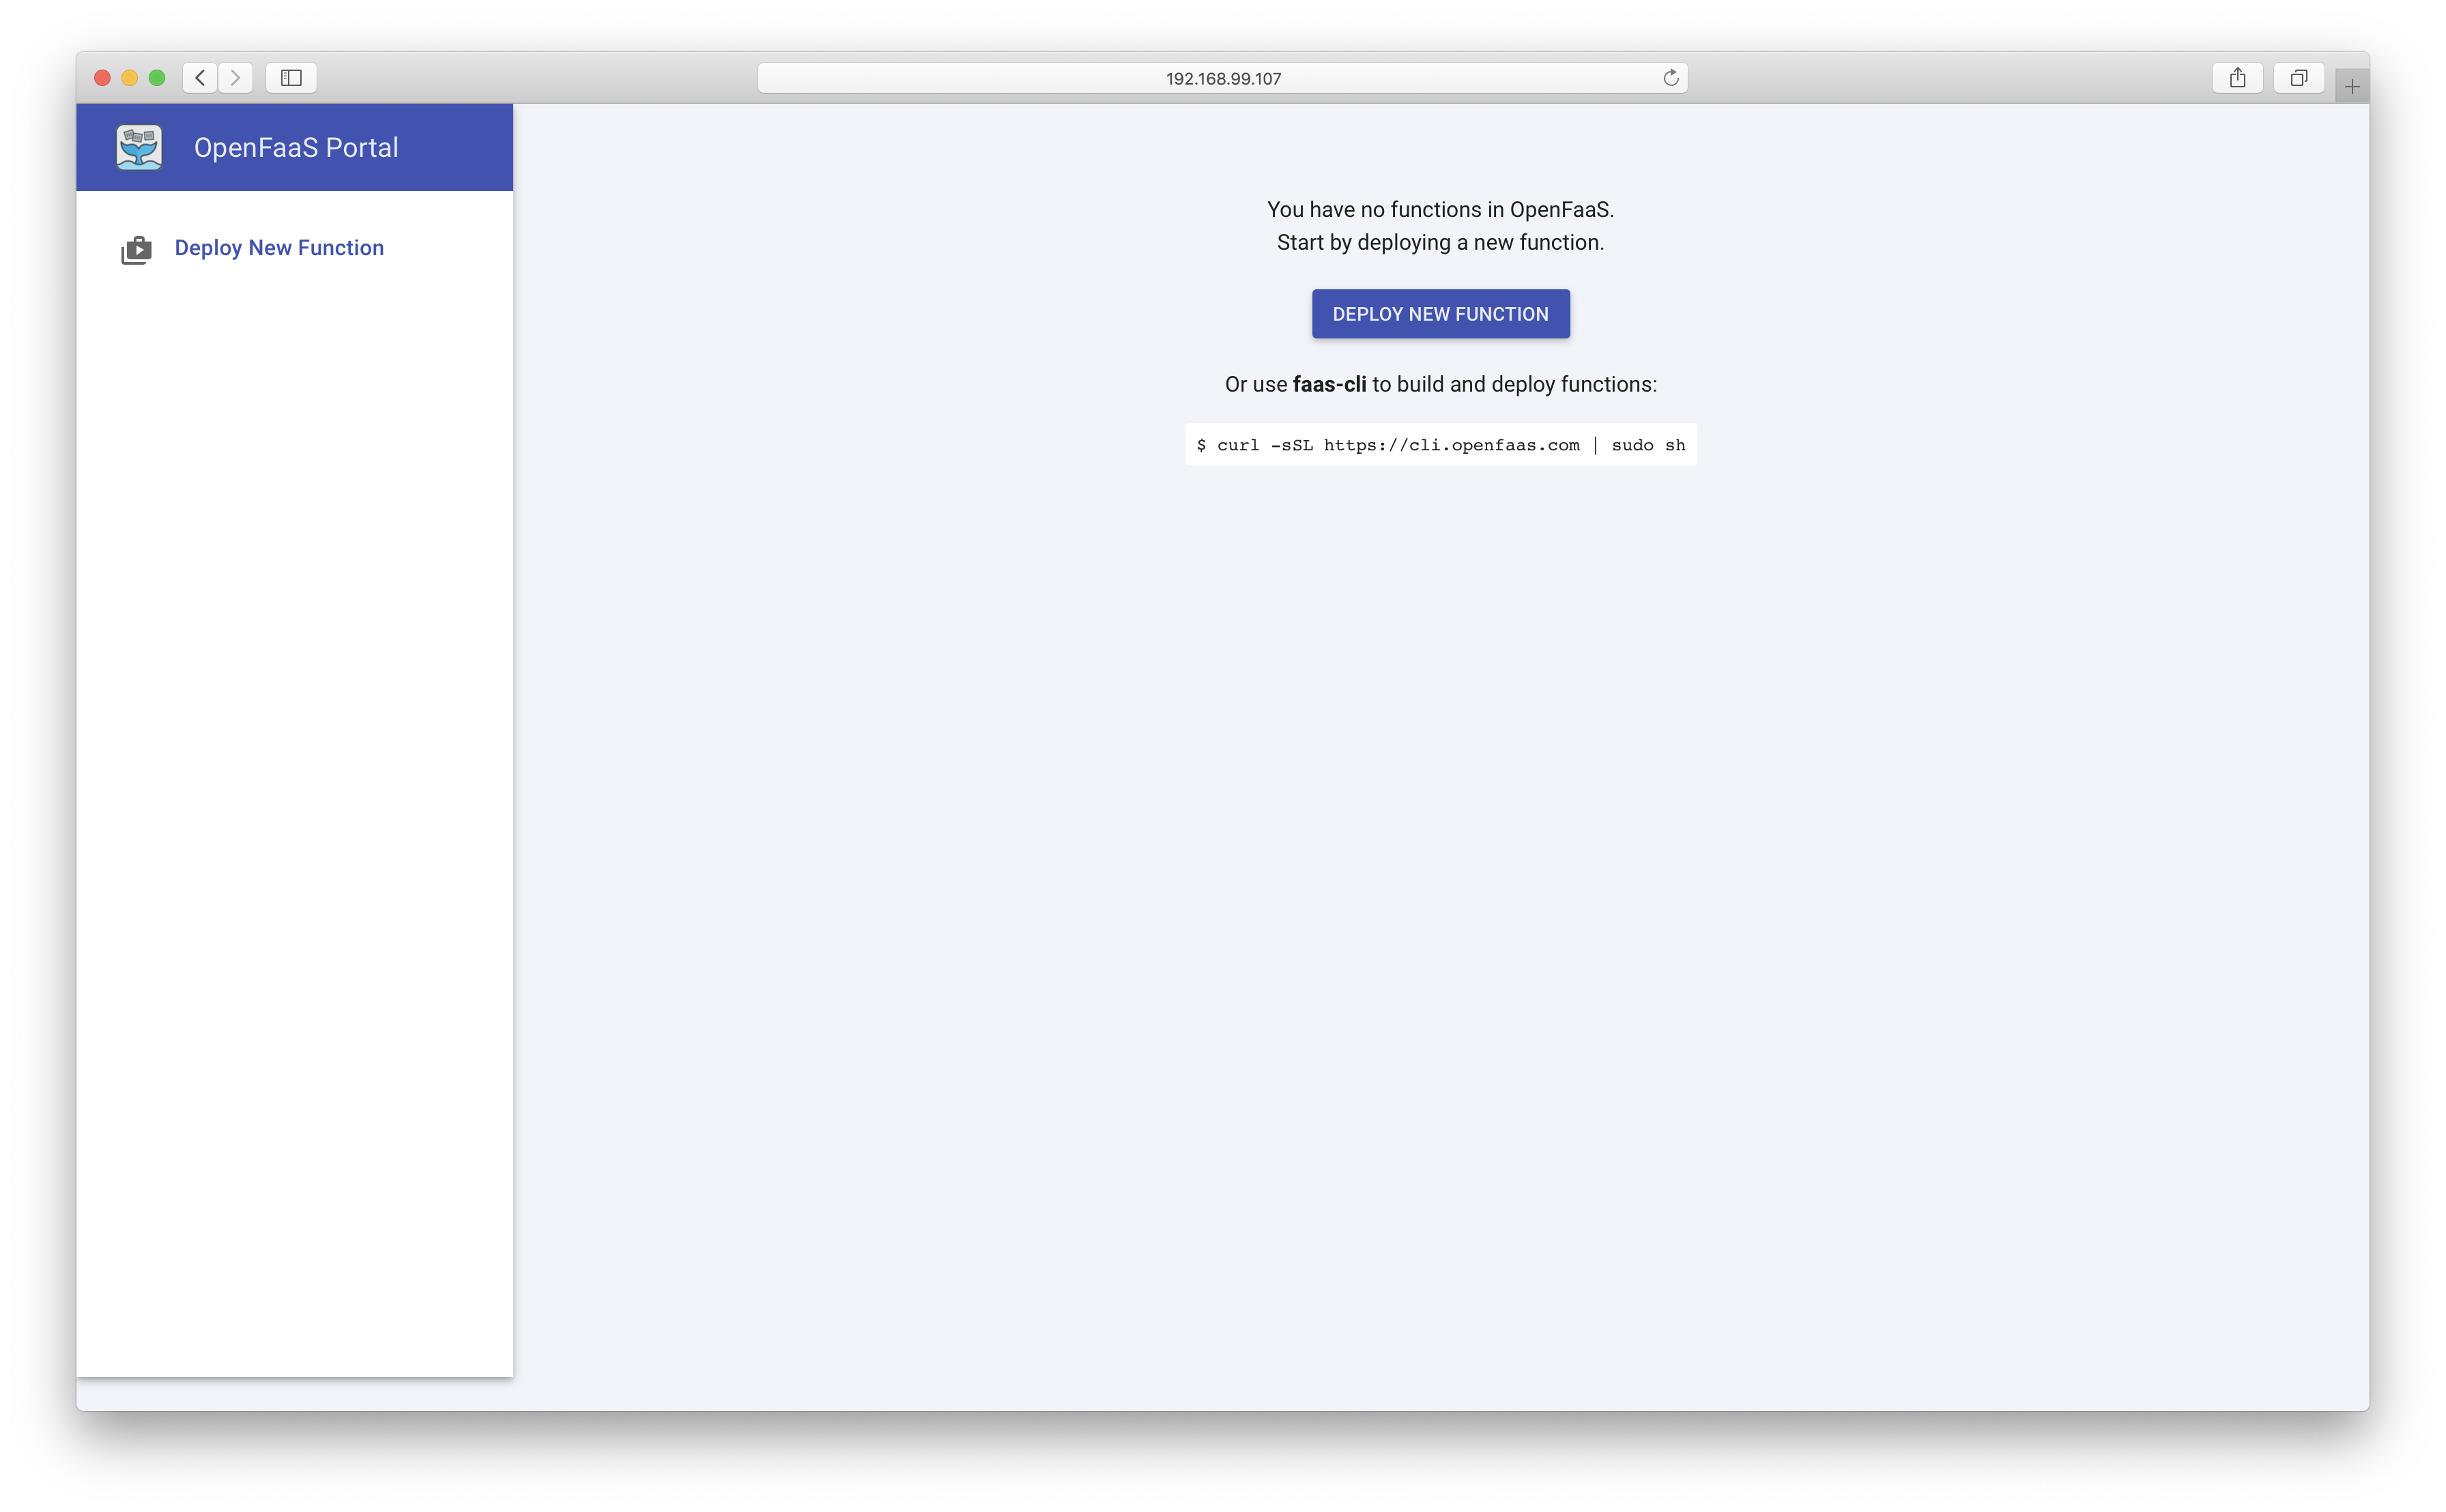
\includegraphics[width=1\textwidth]{img/openfaas-ui.png}
    \caption{OpenFaaS User Interface}
    \label{fig:openfaas-ui}  
\end{figure}

\subsubsection{Command-line tools}
Faas-cli is de command-line tool die beheer van OpenFaaS voorziet aan de hand van de console. Vooraleer van start te kunnen gaan moet de gebruiker inloggen via de Terminal door volgend commando in te voeren. Het paswoord is hetgene dat eerder in de Terminal werd weggeschreven, net zoals het IP adres waarop OpenFaaS draait.
\begin{lstlisting}[language=bash]
$ faas-cli login -g http://$OPENFAAS_URL -u admin -p $PASSWORD
\end{lstlisting}
De command-line tools voorzien dezelfde functionaliteiten als die van de UI. Het is mogelijk om functies te deployen via de CLI. Later in dit onderzoek zal de demofunctie die werd geschreven aan de hand van de command-line tools worden gedeployed.

\subsubsection{Prometheus monitoring}
OpenFaaS voorziet ook monitoring aan de hand van Prometheus, via een Grafana dashboard kunnen verschillende metrics van functies worden bekeken. De configuratie van het dashboard werd reeds voorzien in installatiescript \ref{sec:installatie-openfaas}. Na de configuratie van Prometheus en Grafana kan het dashboard worden geraadpleegd via de GRAFANA\_URL, bijvoorbeeld http://192.168.99.107:32548/dashboard/db/openfaas. In figuur \ref{fig:grafana-dashboard} is het Grafana dashboard zichtbaar dat wordt weergegeven bij het openen van de link. Alvorens dit scherm kan geraadpleegd worden dient de gebruiker in te loggen met de standaard gebruiker ''admin'' met wachtwoord ''admin''.
\begin{figure}
    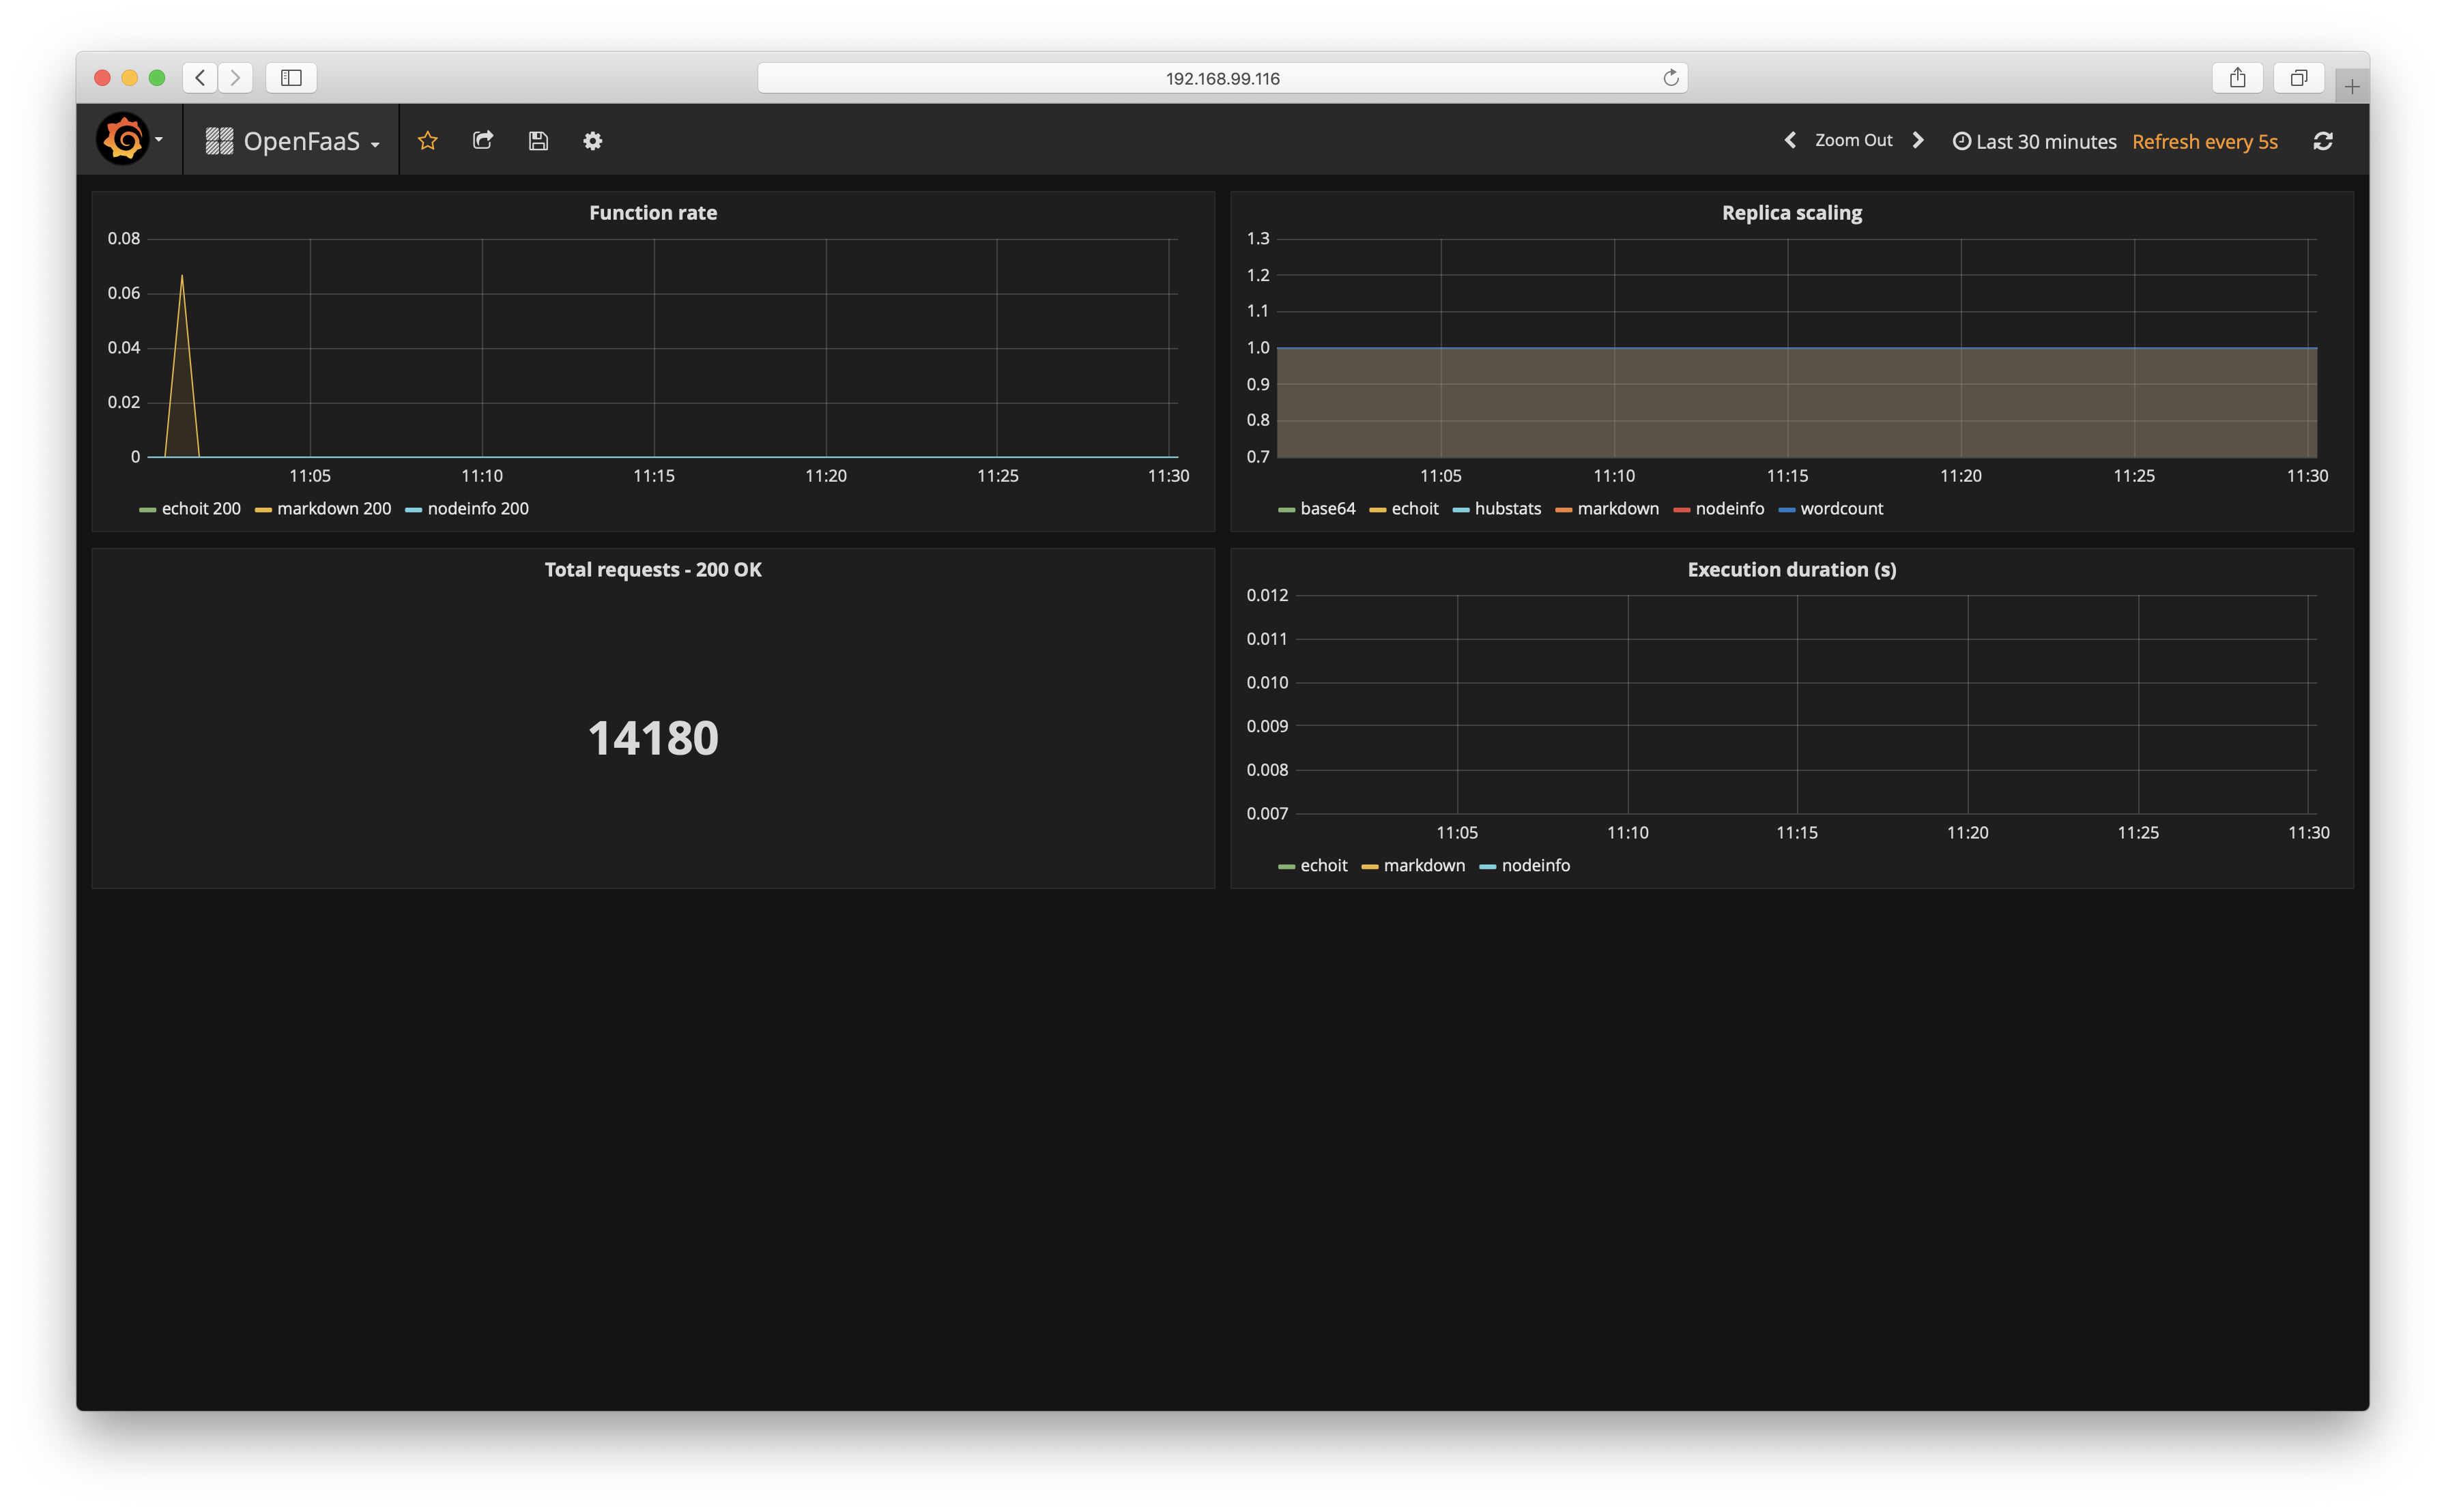
\includegraphics[width=1\textwidth]{img/grafana-dashboard.png}
    \caption{Grafana dashboard}
    \label{fig:grafana-dashboard}  
\end{figure}

\subsection{Deployment demofunctie}

\chapter{Vergelijking frameworks}
\label{ch:vergelijking-frameworks}
In dit hoofdstuk worden de opgezette frameworks met elkaar vergeleken op basis van het uitgevoerde experiment in overeenstemming met de requirements van Nubera. Beide frameworks worden uitvoerig behandeld en worden vergeleken op basis van dezelfde requirements. Dit hoofdstuk geeft de aanzet voor het vormen van een conclusie op de onderzoeksvraag en bijhorende deelonderzoeksvragen. De waarnemingen die in dit hoofdstuk aan bod komen werden allemaal waargenomen bij het opzetten van de Proof of Concept.

\section{Installatie framework}
\label{sec:vergelijking-installatie}
De installatie van OpenFaaS en Fission zijn gelijkaardig aan elkaar. Beide frameworks voorzien command line tools, voor het beheer ervan, die mee in de installatie zijn opgenomen. De stappen die doorlopen moeten worden voor het installeren van de frameworks zijn terug te vinden in de documentatie en kunnen eveneens worden geautomatiseerd. OpenFaaS beschikt over betere documentatie en how-to's die de installatie beschrijven. Het voordeel bij OpenFaaS is dat er standaard in de installatie reeds enkele features, zoals een user interface, aanwezig zijn. Bij installatie van Fission moet de UI nog apart worden toegevoegd. Gezien de standaard features die OpenFaaS meelevert bij installatie en de duidelijkere documentatie, neemt dit framework hier de voorkeur.

\section{Schrijven van functies}
De manier van functie deployment op beide frameworks verschilt en de vorm waarin de code moet worden geschreven is specifiek per framework. OpenFaaS bijvoorbeeld verwacht het gebruik van een ''handle'' methode die een request verwerkt als input parameter. Fission daarentegen verwacht het gebruik van een ''main'' methode zonder input parameters en gebruikt Flask voor het verwerken van HTTP requests. Functies moeten dus wel steeds worden aangepast aan het framework waarop ze draaien. Dit is jammer omdat op die manier geen generieke functies kunnen geschreven worden die op meerdere frameworks bruikbaar zijn, zo moeten functies vaak herschreven worden voor gebruik op een ander serverless framework. Beide benaderingen verschillen van elkaar en dat wat "best" is moet de ontwikkelaar zelf uitmaken. De frameworks bieden wel dezelfde functionaliteiten als het aankomt op schrijven van functies.

\section{Deployment van functies}
De manier waarop gebruikers functies kunnen deployen varieert tussen beide frameworks. Bij gebruik van OpenFaaS moet de gebruiker eerst voorgedefinieerde templates ophalen en deze aanvullen met de code om functionaliteit te voorzien. Vervolgens wordt er een Docker image gebuild en gepusht naar een Docker registry. Wanneer de image beschikbaar is in de registry, kan deze worden gebruikt om een de functie te deployen op het OpenFaaS framework. De volledige workflow kan worden uitgevoerd met de meegeleverde CLI tools die OpenFaaS aanbiedt. Functies kunnen ook via de UI worden gedeployed via OpenFaaS. Wanneer een functie wordt gedeployed, wordt er per functie een container opgezet waarin deze draait, dit is het standaardgedrag van OpenFaaS. OpenFaaS functies kunnen ook geconfigureerd worden zodat na verloop van tijd, als de functie lang geen requests ontvangt, de container wordt afgezet en weer ingeschakeld bij een nieuwe request. OpenFaaS voorziet de mogelijkheid om functies te definiëren in een YAML bestand en het framework leest hier alle waarden uit voor het deployen van een functie. Fission voorziet dit soort van functie templating met YAML bestanden niet.


Fission functie deployment werkt standaard op een andere manier. Indien een gebruiker een nieuwe functie wilt deployen dan moet deze eerst een environment aanmaken, specifiek voor de programmeertaal waarin de functie geschreven is. Vervolgens kan de gebruiker de functie deployen en de code (het bestand dat de code bevat met juiste extensie) meegeven zodat deze wordt gebruikt bij het uitvoeren van de functie. Na het deployen van een functie wordt er ook een route gedefinieerd zodat de functie kan worden aangeroepen via HTTP requests. Fission functies tonen een verschillend standaardgedrag ten opzichte van OpenFaaS. Wanneer een functie wordt gedeployed met default instellingen dan zal telkens wanneer deze wordt aangeroepen de code worden ingeladen in de environment containers en deze zullen de code uitvoeren. Om OpenFaaS en Fission op een gelijkaardige manier te vergelijken, werd het gedrag van OpenFaaS nagebootst. Fission laat toe om extra parameters te definiëren bij het deployen van functies, zo kan de gebruiker ervoor kiezen om het ''executortype'' aan te passen en ervoor te kiezen om de functie in een aparte container te draaien zoals aangehaald in sectie \ref{sec:fission-executors}. Het deployen van functies met een executortype van het type newdeploy komt overeen met de standaard deployment bij OpenFaaS.


Beide frameworks zijn erg gebruiksvriendelijk in het deployen van functies. Het voordeel bij Fission is dat het de mogelijkheid biedt om een route te creëren met een naam naar keuze voor het aanroepen van een functie. De route is een URL die wordt toegevoegd aan de Fission router en HTTP requests doorstuurt naar bijhorende functie. Het is ook interessant dat beide frameworks custom Docker containers toelaten die de gebruikers kunnen maken en gebruiken.
De deployment van functies is zeer specifiek, het is moeilijk een objectief oordeel te vellen over wat nu het beste zou zijn. Zoals eerder gezegd zijn beide frameworks erg gebruiksvriendelijk en is de deployment van functies een persoonlijk aspect afhankelijk van de gebruikers.

\section{Uitvoeringstijd van functies}
\label{sec:vergelijking-uitvoeringstijd}
Om inzicht te krijgen in het verschil in uitvoeringstijd van functies op beide frameworks werd de uitvoeringstijd van de zelfgeschreven Python demofunctie gemeten op beide frameworks. Daarnaast werd ook de uitvoeringstijd van een eenvoudige functie, nl. een ''Hello World'' functie, gemeten. De metingen uit bijlage \ref{sec:uitvoeringstijd-demofunctie} en bijlage \ref{sec:uitvoeringstijd-hello-world} worden vergeleken op basis van  berekeningen uitgevoerd in R. Onderstaande boxplots en tabellen geven inzicht in de metingen. De metingen werden uitgevoerd in een beheerste omgeving, nl. een Minikube cluster die eerder in dit onderzoek werd beschreven. De functies gedeployed op de frameworks draaien allen in een geïsoleerde container die specifiek voor één enkele functie wordt gebruikt, hierdoor worden cold starts vermeden en hoeft hier bij de data-analyse geen rekening gehouden worden. Daarnaast werden de metingen ook achtereenvolgens uitgevoerd, hierdoor kan aangenomen worden dat de datasets representatief zijn.

\newpage
\subsection{Uitvoeringstijd zelfgeschreven Python demofunctie}
De metingen op basis van dataset \ref{sec:uitvoeringstijd-demofunctie} geven inzicht in het verschil tussen uitvoeringstijd van de demofunctie op beide frameworks. Boxplot \ref{fig:boxplot-demo-functie} stelt de verwerkte gegevens visueel voor. De bekomen boxplot, centrum- en spreidingsmaten geven inzicht in het verschil tussen beide frameworks. Op  basis van de centrummaten is te zien dat de mediaan alsook het gemiddelde lager ligt bij Fission dan bij OpenFaaS, de demofunctie kent over het algemeen een iets kortere uitvoeringstijd bij Fission. Bij OpenFaaS zijn ook meer uitschieters terug te vinden maar dit is een factor waar niet op blindgestaard mag worden aangezien de functie gebruikmaakt van een API met authenticatie, deze kan mogelijks de uitschieters verklaren. Om een onderbouwd besluit te vorm wordt in volgende sectie de uitvoeringstijd van een simpele ''Hello World'' functie vergeleken, uitgevoerd op beide frameworks.
\begin{figure}
    \centering
    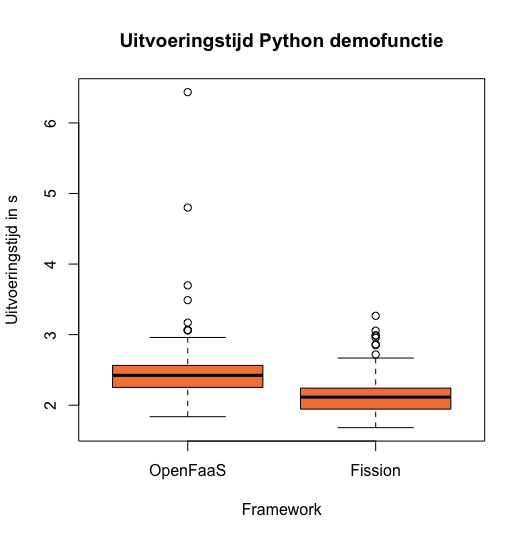
\includegraphics[width=0.6\textwidth]{img/boxplot-uitvoeringstijd-demofunctie.png}
    \caption{Boxplot uitvoeringstijd zelfgeschreven Python functie.}
    \label{fig:boxplot-demo-functie}
\end{figure}

\begin{tabular}{@{}lll@{}}
    \toprule
    & \textbf{OpenFaaS} & \textbf{Fission} \\ \midrule
    \textbf{Min.} & 1.837 & 1.682 \\
    \textbf{1st Qu.} & 2.253 & 1.946 \\
    \textbf{Median} & 2.423 & 2.114 \\
    \textbf{Mean} & 2.473 & 2.146 \\
    \textbf{3rd Qu.} & 2.564 & 2.242 \\
    \textbf{Max.} & 6.436 & 3.267 \\
    \textbf{Stdev.} & 0.423 & 0.267 \\ \bottomrule
\end{tabular}


\subsection{Uitvoeringstijd Hello World Python demofunctie}
De metingen op basis van dataset \ref{sec:uitvoeringstijd-hello-world} geven inzicht in het verschil tussen uitvoeringstijd van de eenvoudige ''Hello World'' functie op beide frameworks. Boxplot \ref{fig:boxplot-hello-functie} stelt de verwerkte gegevens visueel voor.
De boxplot die bekomen wordt door het vergelijken van de uitvoeringstijd, de spreidings- en centrummaten geven inzicht in het verschil tussen beide frameworks. Bij het evalueren van de centrummaten is alweer te zien dat het gemiddelde en de mediaan hoger ligt bij OpenFaas dan bij Fission. De standaardafwijking daarentegen ligt lager bij OpenFaas waardoor uitvoeringstijd constanter is dan bij Fission. De concentratie van de data bij Fission ligt veel dichter bij de mediaan ten opzichte van de data bij OpenFaaS.
\begin{figure}
    \centering
    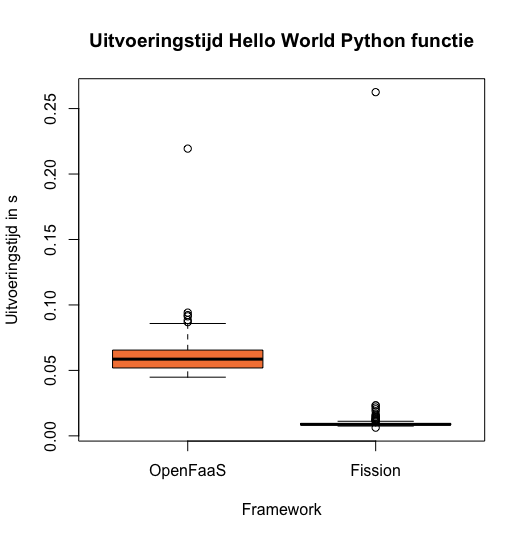
\includegraphics[width=0.6\textwidth]{img/boxplot-uitvoeringstijd-hellofunctie.png}
    \caption{Boxplot uitvoeringstijd Hello World Python functie.}
    \label{fig:boxplot-hello-functie}
\end{figure}

\begin{tabular}{@{}lll@{}}
    \toprule
    & \textbf{OpenFaaS} & \textbf{Fission} \\ \midrule
    \textbf{Min.} & 0.04482 & 0.00626 \\
    \textbf{1st Qu.} & 0.05190 & 0.00832 \\
    \textbf{Median} & 0.05860 & 0.00877 \\
    \textbf{Mean} & 0.06080 & 0.01061 \\
    \textbf{3rd Qu.} & 0.06541 & 0.00945 \\
    \textbf{Max.} & 0.21941 & 0.26255 \\
    \textbf{Stdev.} & 0.01518 & 0.01806 \\ \bottomrule
\end{tabular}

\subsection{Conclusie uitvoeringstijd}
Op basis van voorgaande berekeningen en boxplots is het duidelijk dat het Fission framework een snellere uitvoeringstijd van functies voorziet. Het verschil in uitvoeringstijd bij de zelfgeschreven Python functie valt echter relatief goed mee, het verschil bij de simpele ''Hello World'' functie is aanzienlijk groter. Het verschil lijkt in de opgestelde boxplots vrij groot maar in realiteit is dit echter nauwelijks merkbaar en zorgt dit niet voor grote hinder bij gebruikers. De verschillen in uitvoeringstijd is mogelijks te verklaren doordat beide frameworks gebruikmaken van voorbereide custom containers voor het uitvoeren van functies die door de medewerkers van het project werden gecreëerd. Het kan zijn dat de OpenFaaS container zwaarder is en meer processen draait waardoor de code iets trager uitgevoerd kan worden. De uitvoeringstijd is echter geen doorslaggevende factor voor het kiezen van een interessant framework. Doch kan deze factor in acht worden genomen bij het kiezen van een framework voor applicaties die continue de functies aanspreken en heel snel requests moeten bolwerken.

\section{Gebruik van de frameworks}
\subsection{Documentatie}
De frameworks beschikken beide over een mooie website waarop de documentatie op een duidelijke manier wordt gerepresenteerd. Op het eerste zin ziet de documentatie bij de frameworks er zeer compleet en duidelijk uit maar dit is echter te betwisten. De documentatie over OpenFaaS zat erg goed in elkaar met duidelijke voorbeelden en up-to-date code voor het opzetten van de omgeving als voor het deployen en het beheer van functies. Naast de documentatiewebsite zijn er ook veel bronnen over OpenFaaS terug te vinden zoals demo's of talks op conferenties. De documentatie van Fission daarentegen is beduidend minder kwaliteitsvol dan die van OpenFaaS. Fission beschikt in eerste instantie over relatief weinig documentatie, wat het voor beginners moeilijk maakt om hiermee aan de slag te gaan. De manier waarop bepaalde zaken in Fission werken zijn niet heel duidelijk beschreven in de documentatie en overigens zijn er ook weinig extra bronnen over terug te vinden. OpenFaaS biedt op dit moment de beste en meest duidelijke documentatie aan gebaseerd op eigen mening.

\subsection{User interface}
OpenFaaS voorziet standaard in de installatie een user interface. Gebruikers kunnen via de UI functies deployen en beheren. De instap, voor gebruikers zonder ervaring met FaaS frameworks en functies, is zeer laagdrempelig gezien de duidelijke en eenvoudige UI. Via de interface is het eenvoudig om demofuncties te deployen en deze ook te testen. Bij Fission daarentegen moest de UI na installatie van het framework nog bijkomstig worden geïnstalleerd. De UI van Fission is een ''early alpha'' versie die zelfs niet verenigbaar is met de Fission versie die in dit onderzoek werd gebruikt. De UI kon worden geraadpleegd maar geen enkele functionaliteit ervan bleek te werken. OpenFaaS is duidelijk een winnaar op basis van de huidige user interfaces.

\subsection{Command line tools}
Beide frameworks bieden CLI tools voor het beheer van de infrastructuur. De tools zijn beiden erg gebruiksvriendelijk en voorzien eveneens een duidelijke help functie met uitleg over de commando's. De volledige frameworks zijn te beheren via de command line, dit zorgt ervoor dat zaken makkelijk te reproduceren zijn. De enige bemerking bij dit onderdeel is dat Fission geen ''brew'' package heeft voor het installeren van de Fission CLI tools op macOS in tegenstelling tot OpenFaaS.

\subsection{Monitoring}
Fission en OpenFaaS voorzien standaard Prometheus voor het verzamelen van metrics en monitoring van de omgeving. Beide ondersteunen additionele dashboards die achteraf bovenop Prometheus kunnen worden geïnstalleerd voor het visueel representeren van metrics die werden verzameld. De frameworks scoren allebei goed op dit onderdeel, FIssion voorziet standaard ook Istio voor het management van de services en containers.

\section{Schaalbaarheid functies}
OpenFaaS en Fission schalen functies als de load verhoogd of verlaagd. Wanneer het CPU verbruik van een functiecontainer boven een zekere limiet gaat worden er extra functiecontainers opgezet en worden requests naar functies verdeeld door load-balancing. Vooraleer dit in werking treedt bij Fission moet het executortype worden ingesteld bij deployment van de functie, dit werd al uitvoerig in sectie \ref{sec:fission-executors} behandeld. In de Proof of Concept werd er een demo gegeven waarin functie autoscaling werd getriggerd in het geval van OpenFaaS. De demo gaf mooi weer dat er effectief extra containers werden opgezet als de load verhoogde. De demo van Fission daarentegen was eerder teleurstellend omdat autoscaling niet kon gedemonstreerd worden door onderliggende problemen. Volgens experten zijn de problemen te wijten aan onderliggende componenten, nl. metrics-server voor het verzamelen van metrics omtrent CPU en dergelijke. Beide frameworks voorzien effectief autoscaling desondanks dat dit niet bij allebei kon worden gedemonstreerd. Er wordt vanuit gegaan dat, in een productieomgeving die bestaat uit een Kubernetes cluster met meerdere nodes, de functies autoscalen indien de load hoger wordt. De OpenFaaS demo gaf wel een knap voorbeeld van hoe snel en effectief de autoscaling in zijn werk gaat. Autoscaling biedt een groot voordeel in het beheer van resources, er worden meer recources verbruikt bij veel requests maar wanneer er weer minder requests zijn worden er bijgevolg ook minder resources verbruikt. Het beste framework in dit onderdeel kan moeilijk worden gekozen wegens de mislukte demo. Indien beiden werkten zoals het zou moeten dan blijkt Fission eenvoudiger in het definiëren van additionele parameters voor het instellen van autoscaling. Bij gebruik van Fission is het mogelijk het minimum en maximum aantal pods te definiëren bij het deployen van functies.

%%=============================================================================
%% Conclusie
%%=============================================================================

\chapter{Conclusie}
\label{ch:conclusie}

%% TODO: Trek een duidelijke conclusie, in de vorm van een antwoord op de
%% onderzoeksvra(a)g(en). Wat was jouw bijdrage aan het onderzoeksdomein en
%% hoe biedt dit meerwaarde aan het vakgebied/doelgroep? Reflecteer kritisch
%% over het resultaat. Had je deze uitkomst verwacht? Zijn er zaken die nog
%% niet duidelijk zijn? Heeft het onderzoek geleid tot nieuwe vragen die
%% uitnodigen tot verder onderzoek?

Het gevoerde onderzoek biedt inzicht in alle aspecten omtrent serverless computing waarin Nubera geïnteresseerd is. Alle requirements die werden opgesteld kwamen aan bod en werden vergeleken tussen twee open source frameworks. Daarnaast biedt hoofdstuk~\ref{ch:stand-van-zaken} een theoretische uiteenzetting van het serverless plaatje dat medewerkers en klanten van Nubera warm maakt voor het evolueren naar serverless applicaties.
\\\\
Uit de experimenten blijkt het ene framework beter te scoren dan het andere op basis van enkele vergelijkingen die gevoerd werden in hoofdstuk~\ref{ch:vergelijking-frameworks}. Uit de experimenten blijkt dat Fission beter presteert op basis van executietijd, de demofuncties die op het Fission framework werden gedeployed en aangeroepen hebben een kortere uitvoeringstijd dan de functies op OpenFaaS.
\\\\
OpenFaaS biedt de aangenaamste gebruikerservaring voor gebruikers die nog niet vertrouwd zijn met serverless frameworks. De UI die OpenFaaS standaard meelevert in de installatie is eveneens gebruiksvriendelijk en eenvoudig in gebruik. De interface is intuïtief en vereist eigenlijk geen ervaring met OpenFaaS om hiermee aan de slag te kunnen. Via de UI kunnen functies worden beheerd, gecreëerd en aangeroepen. Standaard zijn er via de interface een aantal community functies beschikbaar die rechtstreeks kunnen worden gedeployed. OpenFaaS voorziet YAML templates voor het definiëren van functies, dit is een overzichtelijke manier om functies te deployen. In tegenstelling tot OpenFaaS voorziet Fission op dit moment nog geen gebruiksvriendelijke UI of YAML templates voor functies. Het vertrouwd raken met OpenFaaS verliep vlotter dan bij Fission dankzij de betere documentatie en de waaier aan extra blogs en video's die hierover te vinden zijn. OpenFaaS is volgens de gevoerde experimenten een duidelijke winnaar op vlak van gebruiksvriendelijkheid. 
\\\\
Beide frameworks zijn vrij makkelijk te installeren maar OpenFaaS voorziet standaard meer componenten. Bij OpenFaaS werkt autoscaling zonder dat er nog extra zaken zoals een metrics-server moeten worden geïnstalleerd in tegenstelling tot Fission. Als beginner is het veel makkelijker van start te gaan met OpenFaaS omdat dit alle componenten bevat die nodig zijn voor een production ready serverless omgeving. Het OpenFaaS framework werkt ''out-of-the-box'' zonder dat er diepgaande kennis van onderliggende infrastructuur nodig is. Fission verwacht wel enig inzicht in de onderliggende infrastructuur en dit schrikt gebruikers die nieuw zijn met het onderwerp mogelijks af.
\\\\
Het gebruik van open source frameworks kent enkele grote voordelen. Gebruikers zijn niet afhankelijk van een cloud provider die de serverless diensten aanbiedt zoals Amazon, Google of Microsoft. Vendor lock-in wordt dus uitgeschakeld waardoor gebruikers niet meer gebonden zijn aan een derde partij. Open source frameworks kunnen gedeployed worden op een eigen infrastructuur in een privaat datacenter on-premises of in een private cloudomgeving. Het gebruik van FaaS oplossingen beperkt het resource verbruik en voorziet autoscaling van functies zonder dat er rekening moet gehouden worden met onderliggende infrastructuur. De frameworks die werden behandeld kunnen ook worden gedeployed op een bestaande Kubernetescluster waardoor er geen nood is aan extra infrastructuur of virtuele servers.
\\\\
In het onderzoek werd getracht het meest interessante open source serverless framework in overeenstemming met de vereisten van Nubera te vinden. Op basis van literair onderzoek, uitgevoerde experimenten en resultatenverwerking werd er tot een besluit gekomen. Het meest veelbelovende framework voor Nubera is OpenFaaS. Zoals reeds werd aangehaald, ligt de uitvoeringstijd van functies hoger bij OpenFaaS dan bij Fission maar het verschil legt echter geen belemmeringen op. Nubera is op zoek naar een serverless framework dat enige maturiteit heeft en goed onderhouden wordt. Daarnaast voldoet OpenFaaS aan alle opgelegde requirements en konden alle functionaliteiten eveneens worden gedemonstreerd. Het onderzoek naar OpenFaaS verliep vlot gezien de duidelijke documentatie en de blogposts die online terug te vinden zijn rond het framework. Aan de ''Nice-to-have'' requirements werd ook voldaan. Klanten van Nubera die interesse hebben in het framework hebben bij OpenFaaS de mogelijkheid om gebruik te maken van de UI, dit is tot op de dag van vandaag iets waar heel veel bedrijven belang aan hechten. De UI zal klassieke klanten kunnen overtuigen om ook aan de slag te gaan met dit serverless framework. Het Fission framework heeft ook erg veel potentieel maar voelt iets minder ''production ready'' aan als OpenFaaS. Binnen de open source community leeft OpenFaaS op het moment van schrijven ook meer dan Fission, desalniettemin heeft het OpenFaaS project ook bijna tienduizend GitHub stars meer wat toch wel wijst op populariteit.
\\\\
Serverless computing is in opmars en dit was ook te merken tijdens het uitwerken van dit onderzoek. Er verschijnen steeds meer bronnen rond het onderwerp op het internet en steeds meer bedrijven gaan ermee aan de slag. De term serverless zorgt nog steeds voor heel wat opschudding bij mensen die geen inzicht hebben in dit onderwerp. Via deze bachelorproef werden de belangrijkste concepten rond serverless nader verklaard in combinatie met enkele demo's die inzicht geven in de mogelijkheden van twee interessante open source serverless frameworks. Na het lezen van dit verslag heeft de lezer hopelijk heel wat nieuwe kennis opgedaan rond serverless en is deze nu ook instaat zich verder te verdiepen in het onderwerp. Er werden twee veelbelovende open source Kubernetes native serverless platformen behandeld, maar er bestaan nog alternatieven die verder onderzoek meer dan waard zijn. Hopelijk kan deze bachelorproef een aanzet geven voor verder onderzoek naar andere, misschien minder bekende maar veelbelovende, open source serverless frameworks.

%%=============================================================================
%% Bijlagen
%%=============================================================================

\appendix

%%---------- Onderzoeksvoorstel -----------------------------------------------

\chapter{Onderzoeksvoorstel}

Het onderwerp van deze bachelorproef is gebaseerd op een onderzoeksvoorstel dat vooraf werd beoordeeld door de promotor. Dat voorstel is opgenomen in deze bijlage.

% Verwijzing naar het bestand met de inhoud van het onderzoeksvoorstel
%---------- Inleiding ---------------------------------------------------------

\section{Introductie} % The \section*{} command stops section numbering
\label{sec:introductie}
Serverless infrastructuur is alomtegenwoordig en verschillende bedrijven beginnen met het ontdekken van deze technologie. De technologie, die deel uitmaakt van Cloud Computing, nl. FaaS (Function as a Service)  biedt nieuwe mogelijkheden voor ontwikkelaars. Bedrijven zijn reeds bezig met de adoptie van deze technologie en grote spelers zoals Amazon, Microsoft en Google proberen daarop in te spelen door serverless diensten aan te bieden. De bedrijven die op dit moment de diensten aanbieden, zijn reeds welbekende Cloud providers daarnaast zien we ook een opmars in de open-source wereld waarin verschillende ontwikkelaars bezig zijn met het ontwikkelen van open-source serverless frameworks.


De serverless benadering (FaaS) is nog volop in ontwikkeling en nog heel recent, de meeste relevante bronnen omtrent serverless zijn niet ouder dan twee jaar wat er dus op wijst dat dit in de toekomst nog aan grote populariteit kan winnen. Om een beter begrip van serverless te geven samen met de mogelijkheden dat het met zich meebrengt is het zinvol hierover een onderzoek te voeren. 


Dit onderwerp werd in samenwerking met het stagebedrijf besproken en uit verdere interesse in deze nieuwe technologie wordt hierop verder gewerkt. De huidige serverless providers werken nu allemaal in een Cloud gebaseerde omgeving, het lijkt interessant om te onderzoeken of hier alternatieven voor zijn. Sommige bedrijven kiezen er vandaag bewust nog voor om niets van resources te migreren naar de Cloud om allerhande redenen, doch willen zij de voordelen van FaaS ook kunnen toepassen in ontwikkeling. De mogelijkheid om op locatie of in een private cloud een FaaS infrastructuur op te zetten is een interessant onderzoek voor zowel het bedrijf als de student. Met een Proof-of-Concept wordt dit soort infrastructuur opgezet om een hands-on demo te kunnen voorzien dat meer inzicht geeft in wat er al dan niet mogelijk is.


De doelstelling is zoals eerder vermeld een volledig onderzoek naar de mogelijkheden van serverless infrastructuren op locatie of in een private cloud. Het onderzoek bestaat uit een een theoretische benadering die gestaafd wordt door een proof-of-concept waarin onderzochte tools en frameworks in gedemonstreerd worden.


\textbf{Onderzoeksvraag: 
    Wat omvat serverless infrastructuren en welke mogelijke open-source projecten bestaan als alternatief voor de huidige serverless infrastructuren die Cloud providers aanbieden?}
\begin{itemize}
  \item Wat is een serverless infrastructuur?
  \item Wat zijn de voor- en nadelen van een serverless infrastructuur?
  \item Wat is het verschil met traditionele infrastructuur?
  \item Welke technologieën maken serverless infrastructuur mogelijk?
  \item Welke open-source alternatieven bestaan er?
  \item Wat is het verschil tussen traditionele en next-gen applicaties?
  \item Welke voordelen bieden next-gen applicaties?
  \item Rol van containers in het verhaal?
  \item Rol van microservices?
  \item Waarom kan de huidige infrastructuur hier al dan niet voor instaan of waarom zouden we beter migreren naar een serverless oplossing?
  \item Waarom moeten IT-bedrijven naar serverless architecturen of next-gen applicaties evolueren?
\end{itemize}

%---------- Stand van zaken ---------------------------------------------------

\section{State-of-the-art}
\label{sec:state-of-the-art}

Serverless is een technologie die in opmars is en verschillende IT-bedrijven springen nu volledig op dit concept. Alvorens in detail op dit onderwerp in te gaan is het belangrijk om een algemeen beeld te hebben hierover. Deze sectie handelt over wat serverless en FaaS inhoudt, wat de voordelen/nadelen zijn, welke bedrijven reeds bezig zijn met deze concepten en welke benaderingen er in ontwikkeling zijn.

\subsection{Wat is Serverless?}
Serverless is een computing technologie dat volledige controle over infrastructuur geeft aan de cloud provider. De provider staat in voor het volledige management van containers waarop ontwikkelaars functies uit kunnen voeren. Door dit te doen zorgt deze architectuur ervoor dat het niet meer nodig is om systemen voortdurend te laten draaien en enkel te laten werken als er event-driven taken moeten worden uitgevoerd. Deze architectuur laat het toe op een eenvoudige manier een schaalbare applicatie uit te rollen. Serverless stelt ontwikkelaars in staat om code te schrijven, op te laden en uit te voeren zonder enige zorg over de onderliggende infrastructuur. Deze technologie kent talloze mogelijkheden die daarenboven ontwikkeling van applicaties tot tweemaal sneller kan maken. \autocite{Stigler2017} Een andere benaming die vaak terugkomt in serverless computing is FaaS oftewel \textit{Function as a Service} dit wordt door \textcite{VanEyck2018} omschreven als een vorm van serverless computing waar de cloud provider instaat voor het management van de resources, de levenscyclus en de event-driven uitvoering van functies die door de gebruiker voorzien werden.

\subsection{Voordelen}
Werken met een serverless omgeving zoals AWS Lambda kan volgens \textcite{Perez2018} de kost van resources voor 70\% verminderen naargelang het aantal gebruikers stijgt met garantie op even goede performance. Serverless biedt de mogelijkheid om snel uit te breiden wanneer dit nodig is zonder dat hier performantie van afhankelijk is. Grote bedrijven zoals Netflix en LinkedIn werken tegenwoordig met microservices in een serverless omgeving, dit verhoogt de flexibiliteit en reduceert de kost aanzienlijk. Daarnaast sluit deze manier van werken aan bij de agile benadering gehanteerd bij softwareontwikkeling. \autocite{Villamizar2017} Een van de grote voordelen wanneer klanten opteren voor serverless computing is dat ze enkel hoeven te betalen voor de code die effectief uitgevoerd wordt. Wanneer er meer code moet uitgevoerd worden dan laat de provider het toe om op te schalen zonder dat de ontwikkelaar op voorhand rekening moet houden hoeveel geheugen en cpu-tijd nodig zal zijn. De ontwikkelaars kunnen op deze manier focussen op code en niet zozeer op de infrastructuur waarop de code draait, deze verantwoordelijkheid verschuift volledig naar de provider. \autocite{Savage2018}

\subsection{Benaderingen}
Bij het raadplegen van bronnen wordt er vaak over grote cloud providers gesproken zoals AWS, Google Cloud en Microsoft Azure, al deze bedrijven voorzien serverless infrastructuren in de publieke cloud. Een infrastructuur die onderhouden wordt door één van voorgaande kan dus nergens anders uitgerold worden buiten in de publieke cloud. Bedrijven die gebruik willen maken van FaaS infrastructuren op locatie of in de private cloud kunnen gebruik maken van open-source alternatieven. Mogelijke alternatieven voor een serverless infrastructuur zijn OpenFaaS \autocite{Ellis2017} en het Serverless Framework \autocite{Serverless2018}. Naar deze mogelijke alternatieven worden

% Voor literatuurverwijzingen zijn er twee belangrijke commando's:
% \autocite{KEY} => (Auteur, jaartal) Gebruik dit als de naam van de auteur
%   geen onderdeel is van de zin.
% \textcite{KEY} => Auteur (jaartal)  Gebruik dit als de auteursnaam wel een
%   functie heeft in de zin (bv. ``Uit onderzoek door Doll & Hill (1954) bleek
%   ...'')


%---------- Methodologie ------------------------------------------------------
\section{Methodologie}
\label{sec:methodologie}

Allereerst wordt er aan deskresearch gedaan om de nodige informatie omtrent het onderwerp te verzamelen, deze bronnen worden verwerkt in een literatuurstudie die als basis voor dit onderzoek fungeert. Aan de hand van de verzamelde bronnen worden er antwoorden geformuleerd op de theoretische deelonderzoeksvragen. Wanneer er voldoende bronnen zijn verzameld wordt er een laboratoriumonderzoek gevoerd waarin een proof-of-concept wordt uitgewerkt. In deze proof-of-concept wordt er een full stack uitgewerkt met tools zoals: Docker, eventueel Docker Swarm of Kubernetes, eventuele automatiseringstools en een open-source framework voor het opzetten van een FaaS omgeving. Op de opgezette omgeving wordt ook een applicatie uitgerold.

%---------- Verwachte resultaten ----------------------------------------------
\section{Verwachte resultaten}
\label{sec:verwachte_resultaten}

Er wordt verwacht dat deze paper een significante bijdrage kan leveren aan bedrijven die geïnteresseerd zijn in het opzetten van een serverless omgeving. De paper stelt begunstigden in staat een algemeen beeld te krijgen van wat serverless is, wat er bestaat en met welke alternatieven. Er wordt ook gedemonstreerd hoe er zelf een demo-omgeving kan worden opgezet. Op basis van dit document moeten bedrijven een beslissing kunnen nemen of het voor hen zinvol is te evolueren naar serverless infrastructuren.


%---------- Verwachte conclusies ----------------------------------------------
\section{Verwachte conclusies}
\label{sec:verwachte_conclusies}

Er wordt verwacht dat er verschillende open-source alternatieven zijn voor serverless infrastructuren. De demo-opstelling maakt het mogelijk om verschillende benaderingen te vergelijken en geïnteresseerde bedrijven bij te staan bij de keuze om eventueel te evolueren naar serverless infrastructuren.


%%---------- Andere bijlagen --------------------------------------------------
% TODO: Voeg hier eventuele andere bijlagen toe
%\input{...}
\chapter{Broncode}
\section{Installatiescript OpenFaaS}
\label{sec:installatie-openfaas}
\begin{lstlisting}[language=bash]
#!/bin/bash
# Install OpenFaaS
brew install faas-cli

# Install Kubernetes Helm
brew install kubernetes-helm

# Deploy OpenFaaS to Minikube
# 1. Create a service account for tiller
kubectl -n kube-system create sa tiller && \
kubectl create clusterrolebinding tiller --clusterrole \
cluster-admin --serviceaccount=kube-system:tiller
sleep 10

# 2. Install tiller
helm init --skip-refresh --upgrade --service-account tiller
sleep 10

# 3. Create namespaces for OpenFaaS core components and OpenFaaS Functions
kubectl apply -f https://raw.githubusercontent.com/openfaas/faas-netes/master/namespaces.yml
sleep 10

# 4. Add the OpenFaaS helm repository
helm repo add openfaas https://openfaas.github.io/faas-netes/
sleep 10


# 5. Generate a random password
export PASSWORD=$(head -c 12 /dev/urandom | shasum| cut -d' ' -f1)

# 6. Log the password value to the user
echo Password: $PASSWORD

# 7. Create a secret for the generated password and write it to gateway-password.txt
kubectl -n openfaas create secret generic basic-auth \
--from-literal=basic-auth-user=admin --from-literal=basic-auth-password="$PASSWORD"

echo $PASSWORD > gateway-password.txt

# 8. Install OpenFaaS using chart
helm repo update \
&& helm upgrade openfaas --install openfaas/openfaas \
--namespace openfaas --set functionNamespace=openfaas-fn --set basic_auth=true
sleep 10

# 9. Set an environment variable for the OpenFaaS URL: OPENFAAS_URL
export OPENFAAS_URL=$(minikube ip):31112
export URL=$(minikube ip)
echo URL: $OPENFAAS_URL


# Configure Prolmetheus Grafana dashboard
kubectl -n openfaas run \
--image=stefanprodan/faas-grafana:4.6.3 \
--port=3000 \
grafana

kubectl -n openfaas expose deployment grafana \
--type=NodePort \
--name=grafana

GRAFANA_PORT=$(kubectl -n openfaas get svc grafana -o \
jsonpath="{.spec.ports[0].nodePort}")
GRAFANA_URL= \
$URL: $GRAFANA_PORT/dashboard/db/openfaas
\end{lstlisting}
\newpage
\section{Demofunctie OpenFaaS}
\subsection{handler.py}
\label{sec:demofunctie-openfaas}
\begin{lstlisting}[language=python]
import gspread
import sys
from oauth2client.service_account import ServiceAccountCredentials

def next_available_row(worksheet):
    str_list = filter(None, worksheet.col_values(1))
    return str(len(str_list)+1)

def is_empty_string(string):
    if len(string) == 0:
        return True
    else:
        return False

def get_values(worksheet):
    cell_range = 'A1:A'+ next_available_row(worksheet)
    all_cells = worksheet.range(cell_range)
    return all_cells

def handle(request):   
    # Initialize variables for Google API
    data = request
    scope = ['https://spreadsheets.google.com/feeds','https://www.googleapis.com/auth/drive']
    credentials = ServiceAccountCredentials.from_json_keyfile_name('/var/openfaas/secrets/secret-api-credentials', scope)
    client = gspread.authorize(credentials)
    worksheet = client.open("executietijd-demofunctie").sheet1
    next_row = next_available_row(worksheet)

    # Print message visible by users
    if is_empty_string(data):
        string_list = []
        for cell in get_values(worksheet):
            string_list.append(cell.value)
        return str(string_list)
    else:
        worksheet.update_acell("A{}".format(next_row), data)
        string_output = "This function wrote " + data + " to Google Spreadsheets!"
        return string_output
\end{lstlisting}

\newpage
\subsection{serverless-demo.yml}
\label{sec:serverless-demo.yml}
\begin{lstlisting}
provider:
  name: openfaas
  gateway: http://192.168.99.119:31112
functions:
  serverless-demo:
    lang: python
    handler: ./serverless-demo
    image: lennertmertens/serverless-demo:latest
    secrets:
      - secret-api-credentials
\end{lstlisting}

\subsection{requirements.txt}
\label{sec:requirements.txt}
\begin{lstlisting}
oauth2client
gspread
google-api-python-client
\end{lstlisting}
\newpage
\section{Installatiescript Fission}
\label{sec:installatie-fission}
\begin{lstlisting}[language=bash]
#!/bin/bash
echo > artifacts.txt
## Minikube enable metrics-server
minikube addons enable metrics-server

## Installeer brew packages
brew install kubernetes-helm

## Configureer Kubernetes cluster
# 1. Maak tiller service account
kubectl -n kube-system create sa tiller && \
kubectl create clusterrolebinding tiller --clusterrole \
cluster-admin --serviceaccount=kube-system:tiller

# 2. Initialiseer tiller service account
helm init --skip-refresh --upgrade --service-account tiller

## Installeer Fission
# 1. Update Helm repo en voeg Fission namespaces toe
helm repo update && \
helm install --name fission --namespace fission \
--set serviceType=NodePort,routerServiceType=NodePort \
https://github.com/fission/fission/releases/download/1.2.0/\
fission-all-1.2.0.tgz
sleep 20

# 2. Installeer Fission CLI tools
if ! ls -f /usr/local/bin/fission;
then
    curl -Lo fission \
    https://github.com/fission/fission/releases/download\
    /1.2.0/fission-cli-osx \
    && chmod +x fission && sudo mv fission /usr/local/bin/;
else
    echo "Fission CLI tools zijn reeds geinstallleerd!"
fi

# Stel Fission omgevingsvariabelen in
export FISSION_URL=http://$(minikube ip):31313
echo FISSION_URL=$FISSION_URL >> artifacts.txt
export FISSION_ROUTER=http://$(minikube ip):31314
echo FISSION_ROUTER=${FISSION_ROUTER} >> artifacts.txt

## Installer Fission UI (optioneel)
MINIKUBE_IP=$(minikube ip)
echo -n "Wilt u de Fission UI installeren? [y/n] "
read answer

if [ "$answer" != "${answer#[Yy]}" ]; then
    PAD=$(pwd)
    # 1. Clone de Git repository
    cd ~
    git clone git@github.com:fission/fission-ui.git
    cd fission-ui
    # 2. Deploy de Fission UI
    kubectl create -f docker/fission-ui.yaml
    cd $PAD
    # Schrijf IP adres naar artifacts
    export FISSION_UI=http://$MINIKUBE_IP:31319
    echo FISSION_UI=$FISSION_UI >> artifacts.txt
else
    echo Fission UI wordt niet geinstalleerd!
fi

# Display the file with artifacts to user
cat artifacts.txt
\end{lstlisting}
\newpage
\section{Docker image python-env}
\label{sec:docker-fission}
\subsection{Dockerfile}
\label{sec:dockerfile-fission}
\begin{lstlisting}
FROM alpine:3.5

RUN apk update
RUN apk add --no-cache python python-dev build-base py-pip libev-dev
RUN pip install --upgrade pip
RUN rm -r /root/.cache

COPY . /app
WORKDIR /app
RUN pip install -r requirements.txt

ENTRYPOINT ["python"]
CMD ["server.py"]
\end{lstlisting}

\subsection{requirements.txt}
\label{sec:requirements-fission}
\begin{lstlisting}]
flask ~= 0.12.3
bjoern
httplib2
python-dateutil
requests==2.20.0
redis
hiredis
gevent
oauth2client
gspread
google-api-python-client
\end{lstlisting}

\newpage
\section{Demofunctie Fission}
\subsection{handler.py}
\label{sec:demofunctie-fission}
\begin{lstlisting}[language=python]
import time
import gspread
import oauth2client
from oauth2client.service_account import ServiceAccountCredentials

def next_available_row(worksheet):
str_list = filter(None, worksheet.col_values(3))
return str(len(str_list)+1)

def main():   
# Initialize variables for Google API
scope = ['https://spreadsheets.google.com/feeds',
        'https://www.googleapis.com/auth/drive']
credentials = ServiceAccountCredentials
        .from_json_keyfile_name('/app/credentials.json', scope)
client = gspread.authorize(credentials)
worksheet = client.open("executietijd-demofunctie").sheet1
next_row = next_available_row(worksheet)

# Start timer 
start = time.time()

# Print statement
print "Hello everyone, this is a serverless demo function!"

# Start loop function to measure execution time
a = range(1000000)
b = []
for i in a:
b.append(i*2)

# Stop timer
end = time.time()

# Calculate the execution time of the function in seconds
execution_time= end - start

# Write the execution time to Google spreadsheet
worksheet.update_acell("C{}".format(next_row), execution_time)
return "Hello everyone, this is a serverless demo function!"


\end{lstlisting}
\section{Installatiescript Frameworks}
\label{sec:installatie-frameworks}
\begin{lstlisting}[language=python]
content...
\end{lstlisting}

\chapter{Google spreadsheets setup}
\section{Google API configuratie}
\label{sec:google-api}
Dit hoofdstuk bevat een gedetailleerd stappenplan voor het configureren van een Google API. De Python demofunctie maakt gebruik van de Google API voor het wegschrijven van data naar Google spreadsheets.

\begin{figure}[h]
    \begin{subfigure}{0.5\textwidth}
        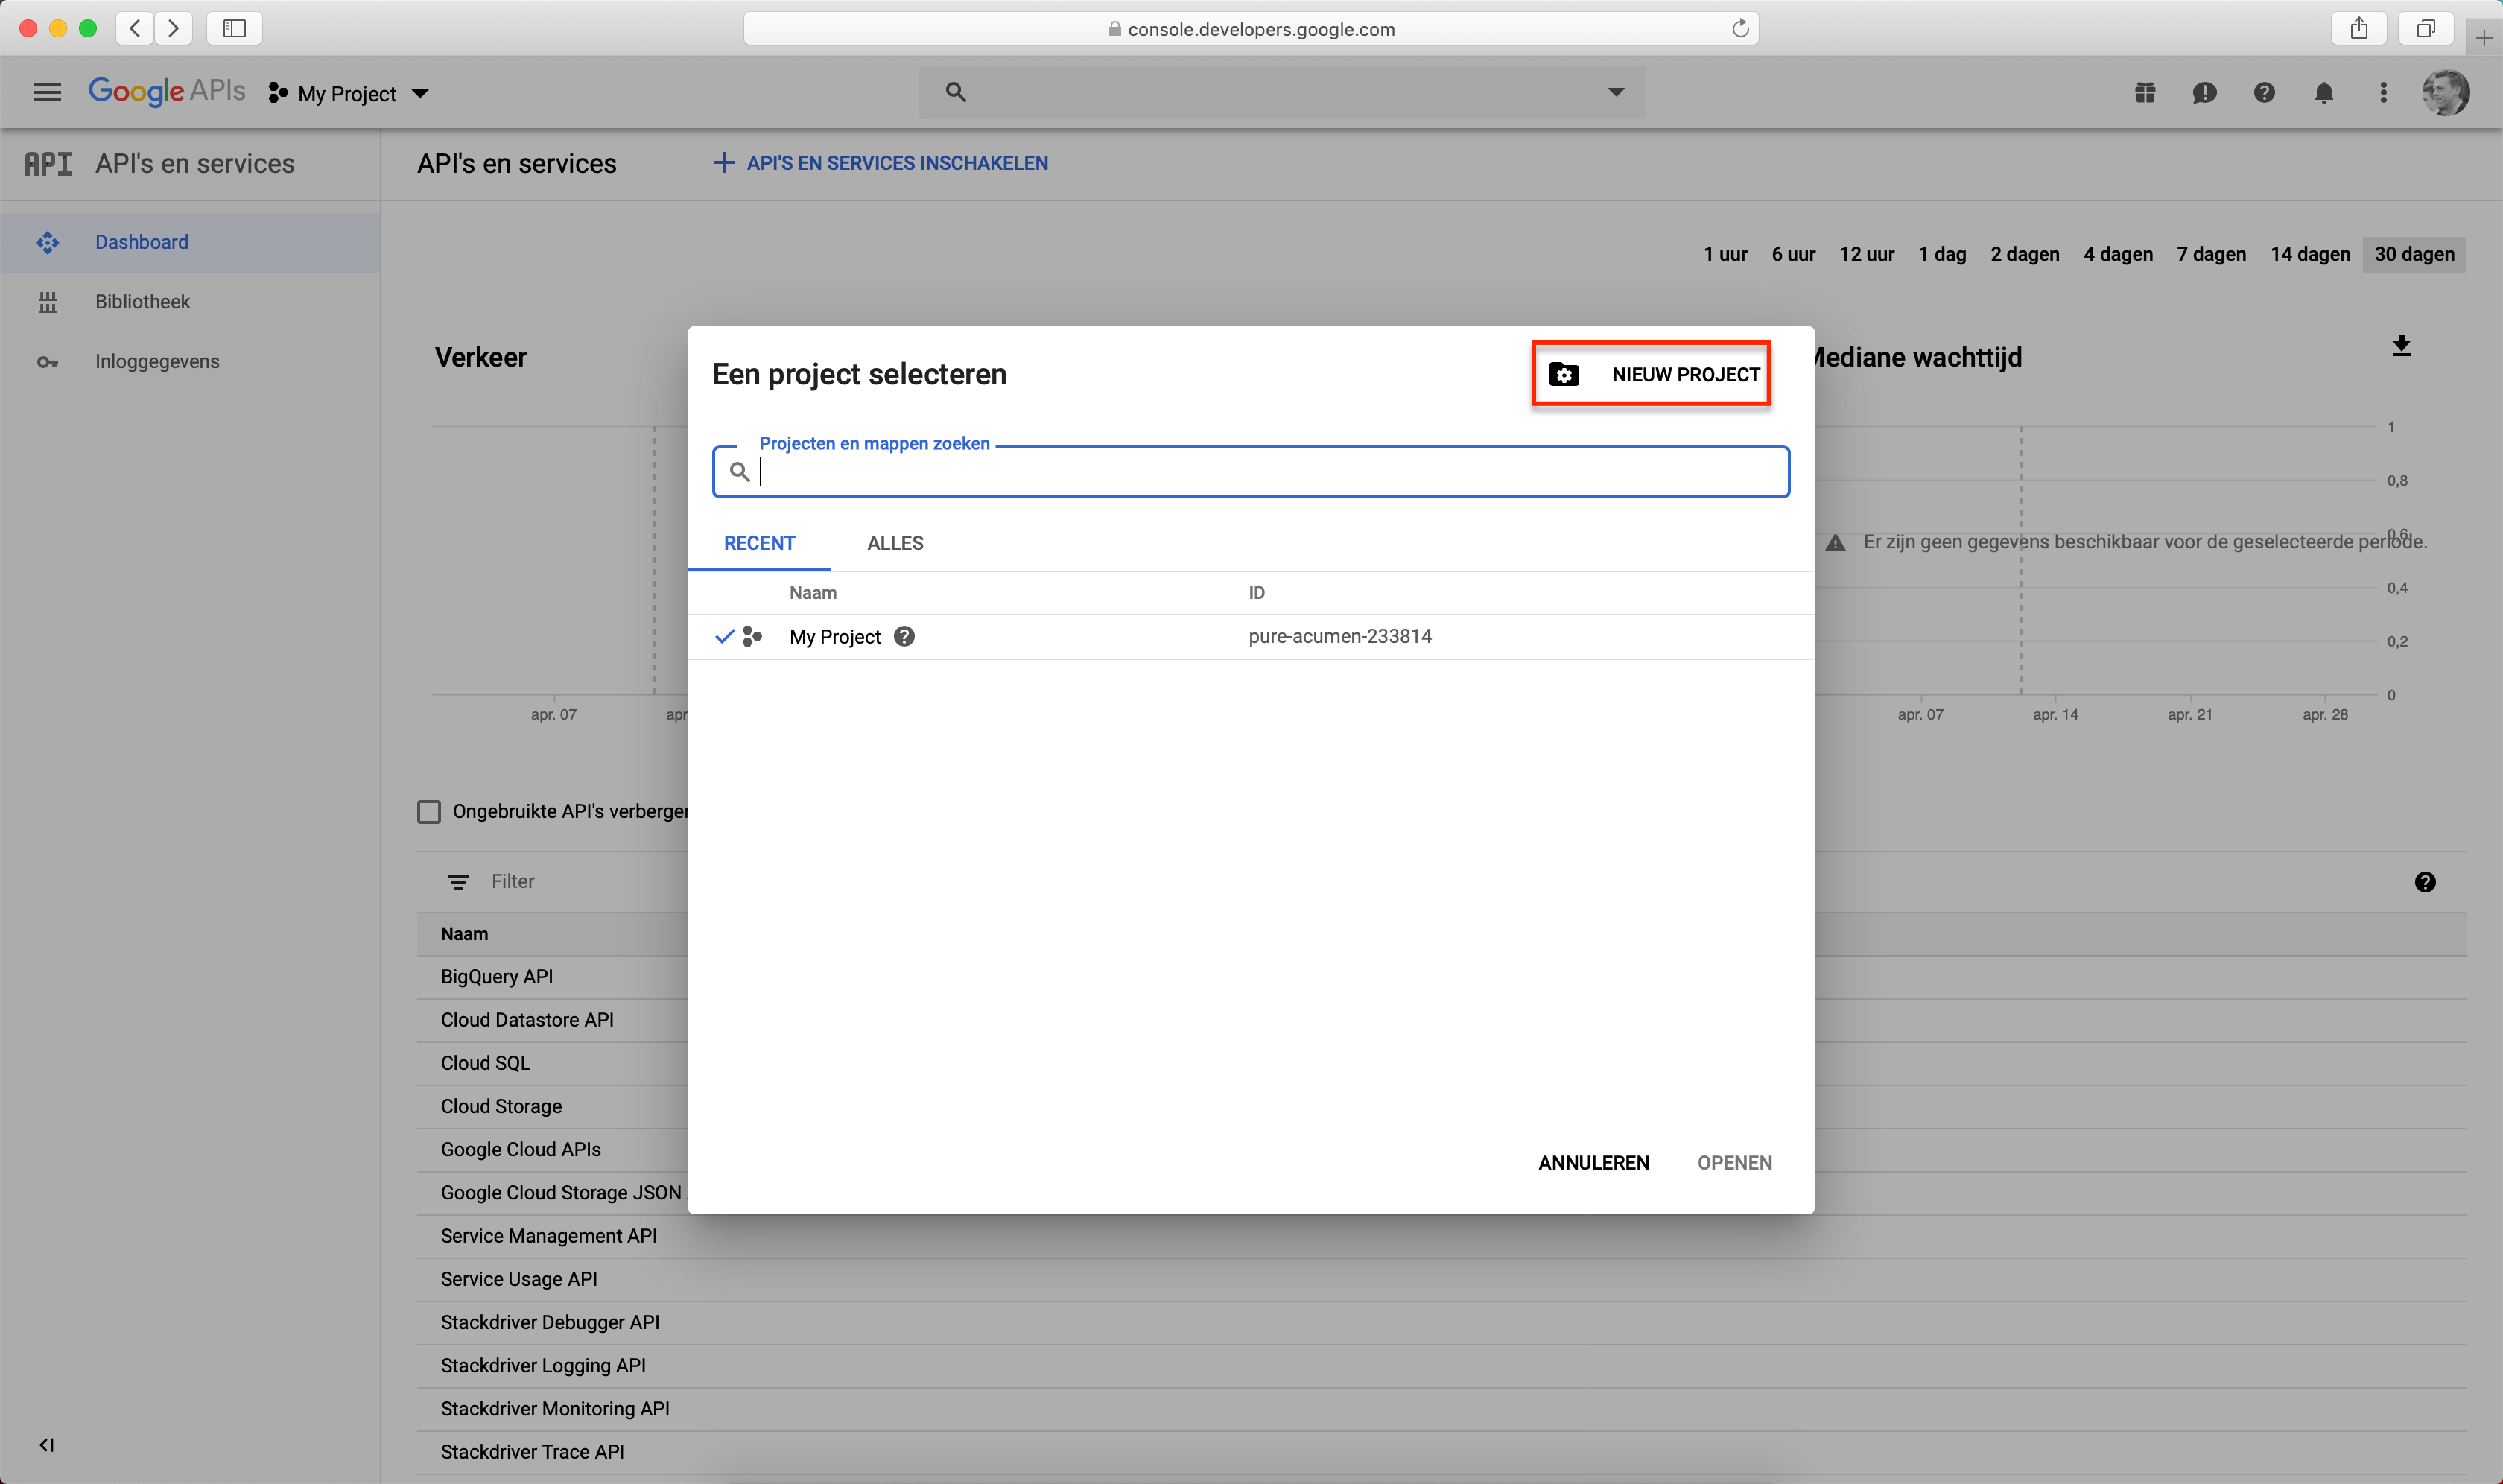
\includegraphics[width=0.9\linewidth,height=4.3cm]{img/google-sheets/gapi-maak-project.png}
        \captionsetup{width=0.8\linewidth}
        \centering
        \caption{Maak een nieuw Google Cloud project via de Google Cloud API console.}
    \end{subfigure}
    \begin{subfigure}{0.5\textwidth}
        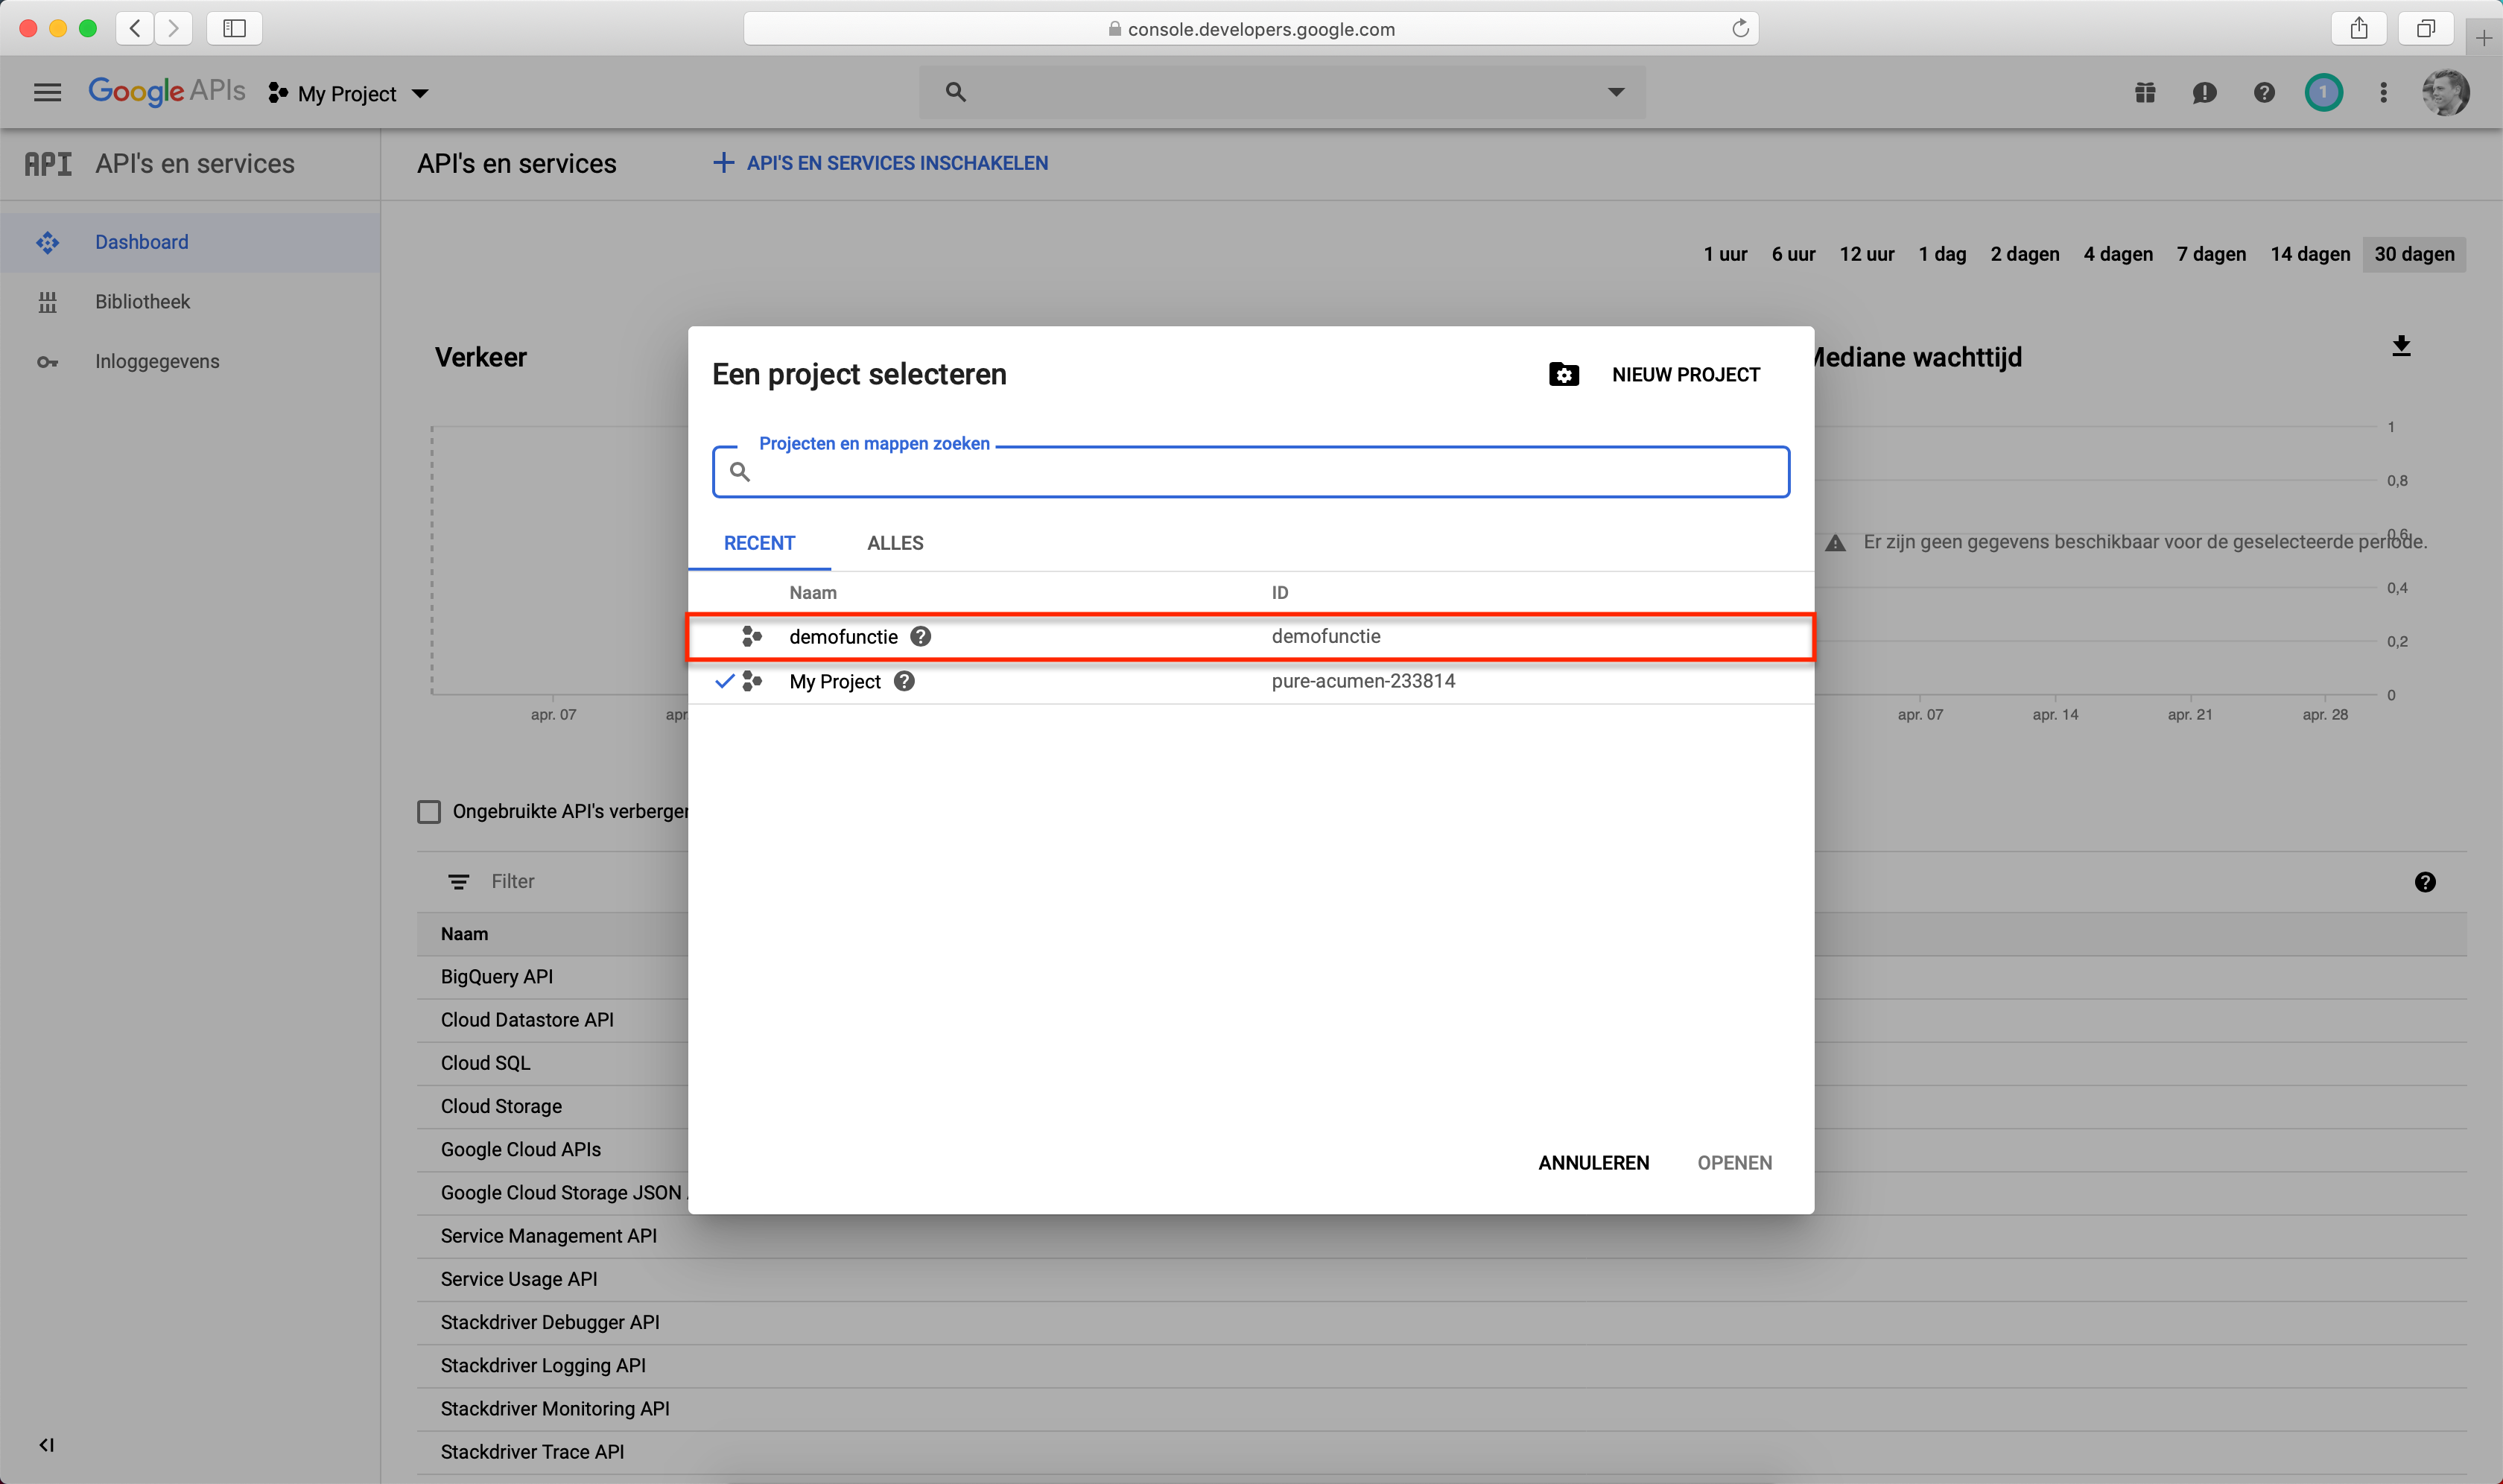
\includegraphics[width=0.9\linewidth,height=4.3cm]{img/google-sheets/gapi-selecteer-project.png} 
        \captionsetup{width=0.8\linewidth}
        \centering
        \caption{Selecteer het project dat zonet aangemaakt werd.}
    \end{subfigure}
\end{figure}
\begin{figure}[h]\ContinuedFloat
    \begin{subfigure}{0.5\textwidth}
        \captionsetup{width=0.8\linewidth}
        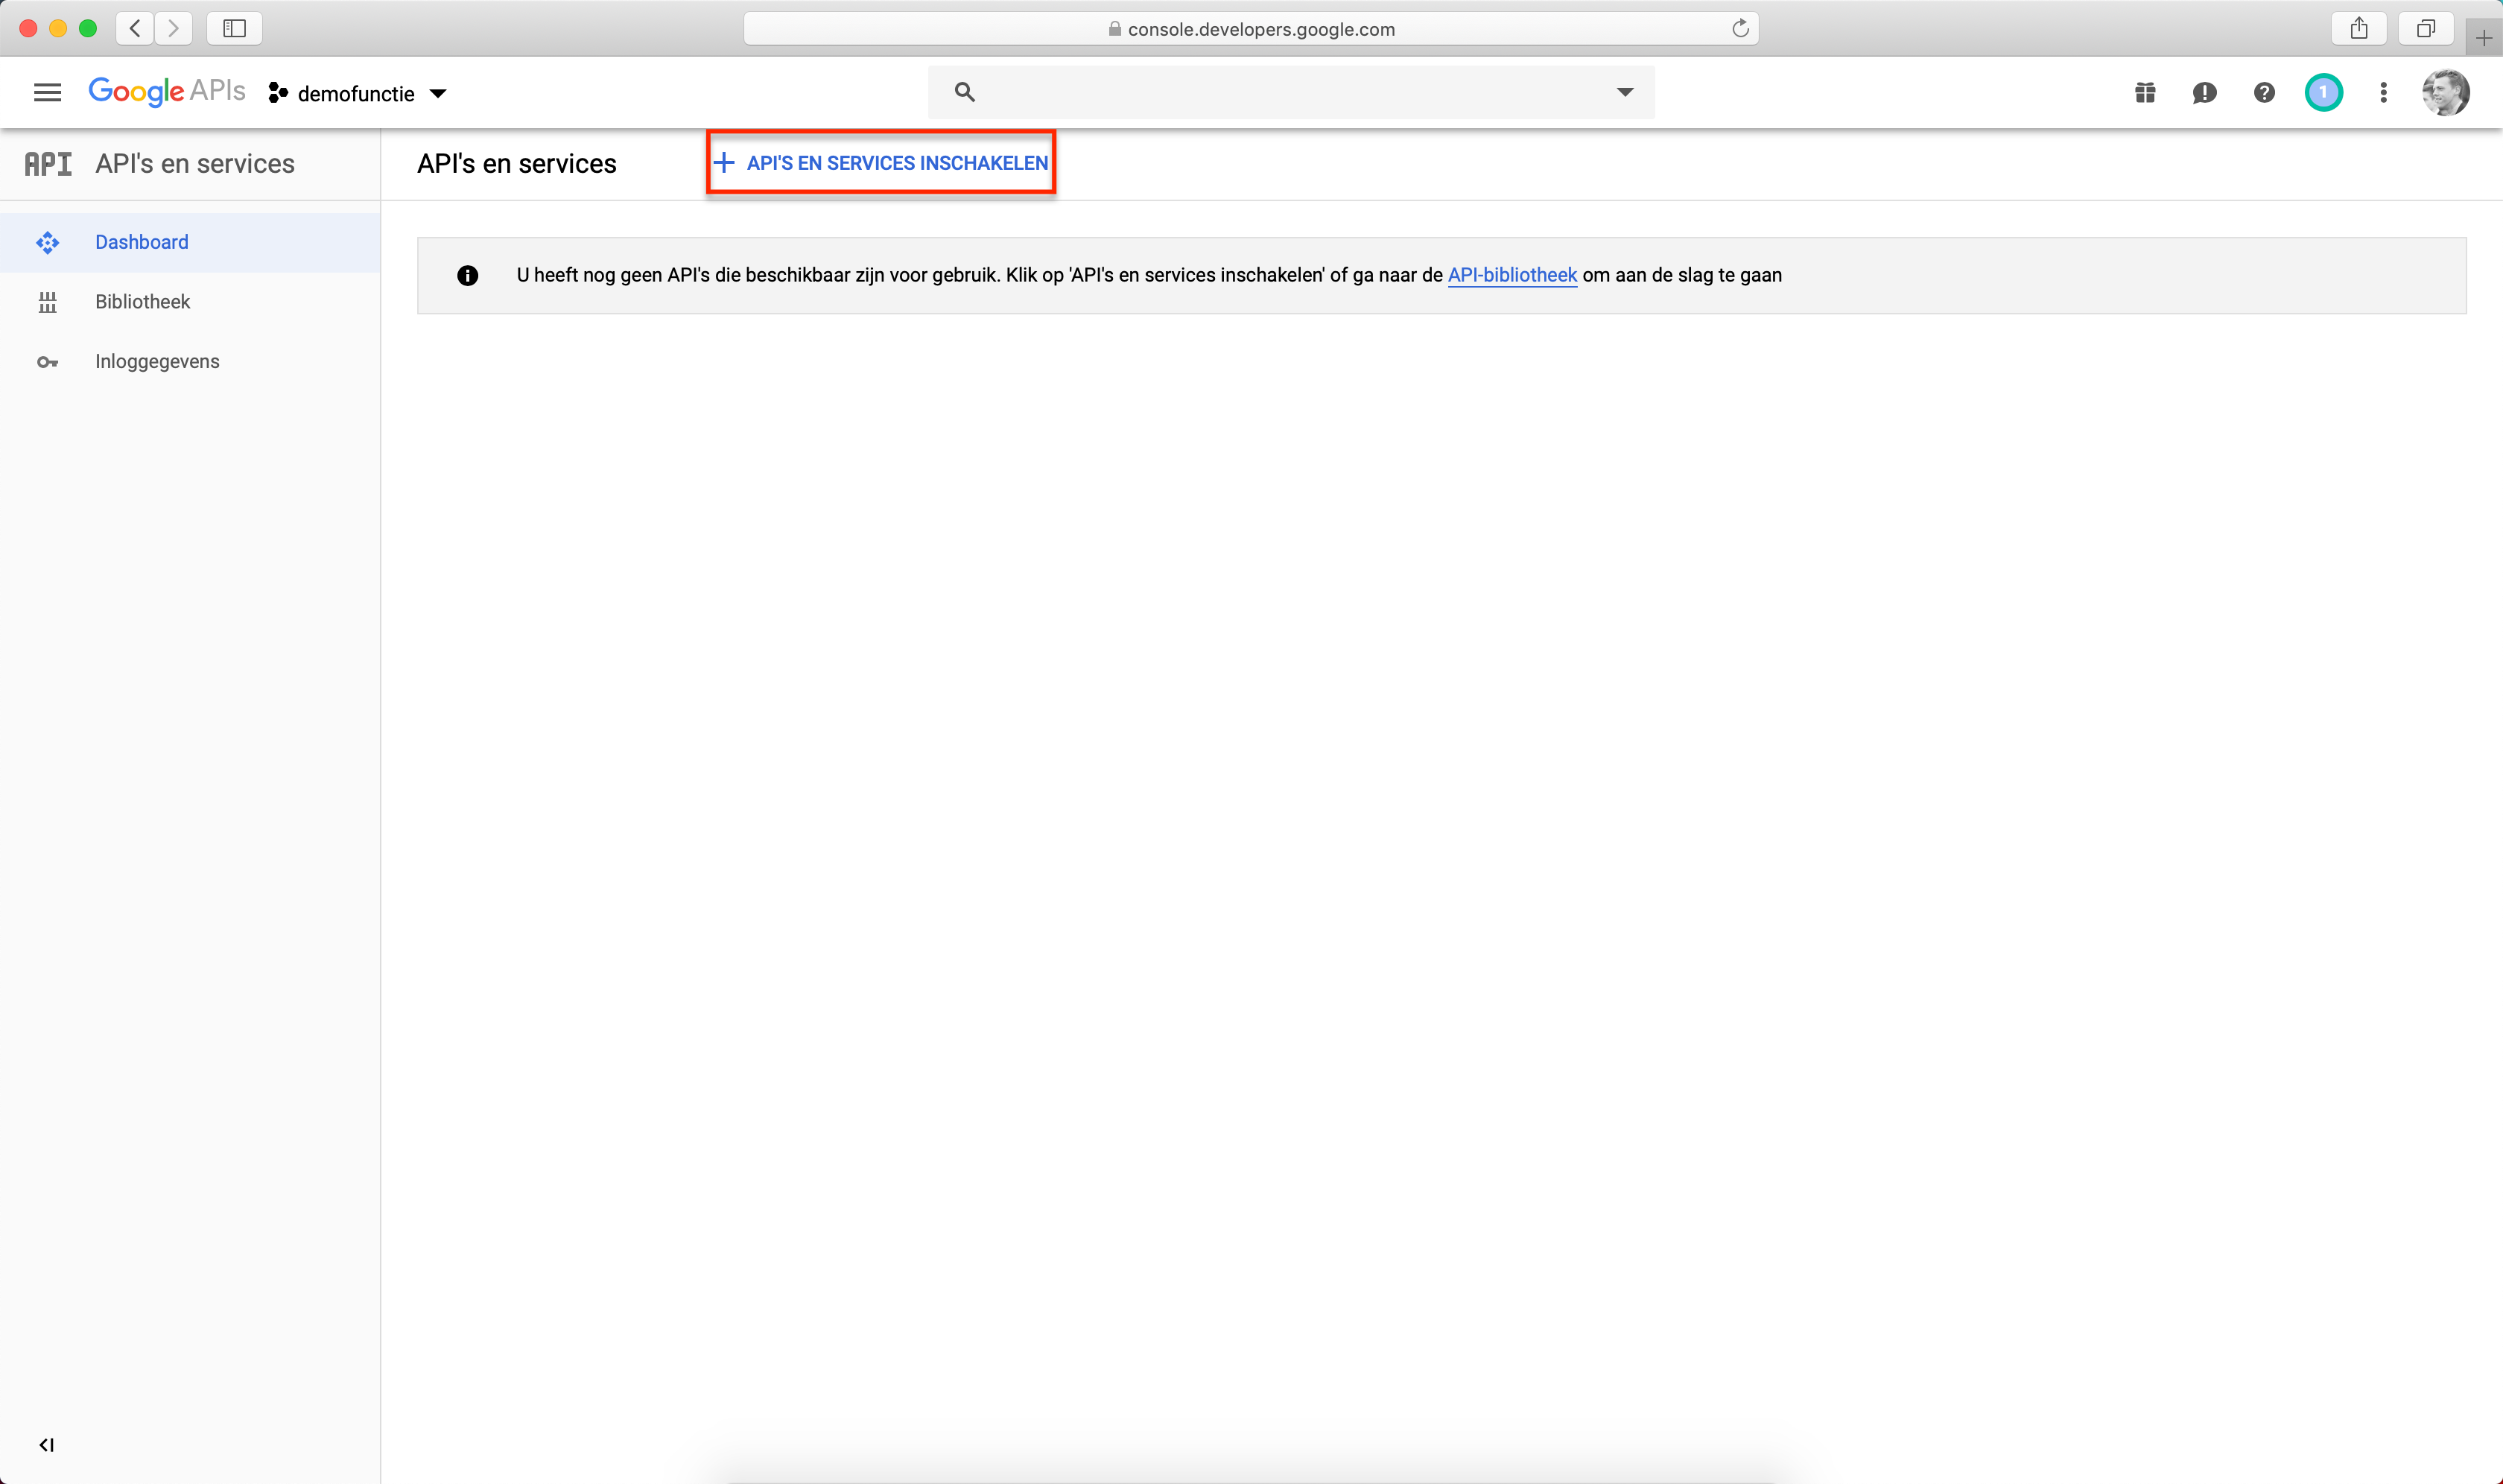
\includegraphics[width=0.9\linewidth,height=4.3cm]{img/google-sheets/gapi-api-inschakelen.png} 
        \centering
        \caption{Kies ervoor om API en services in te schakelen.}
    \end{subfigure}
    \begin{subfigure}{0.5\textwidth}
        \captionsetup{width=0.8\linewidth}
        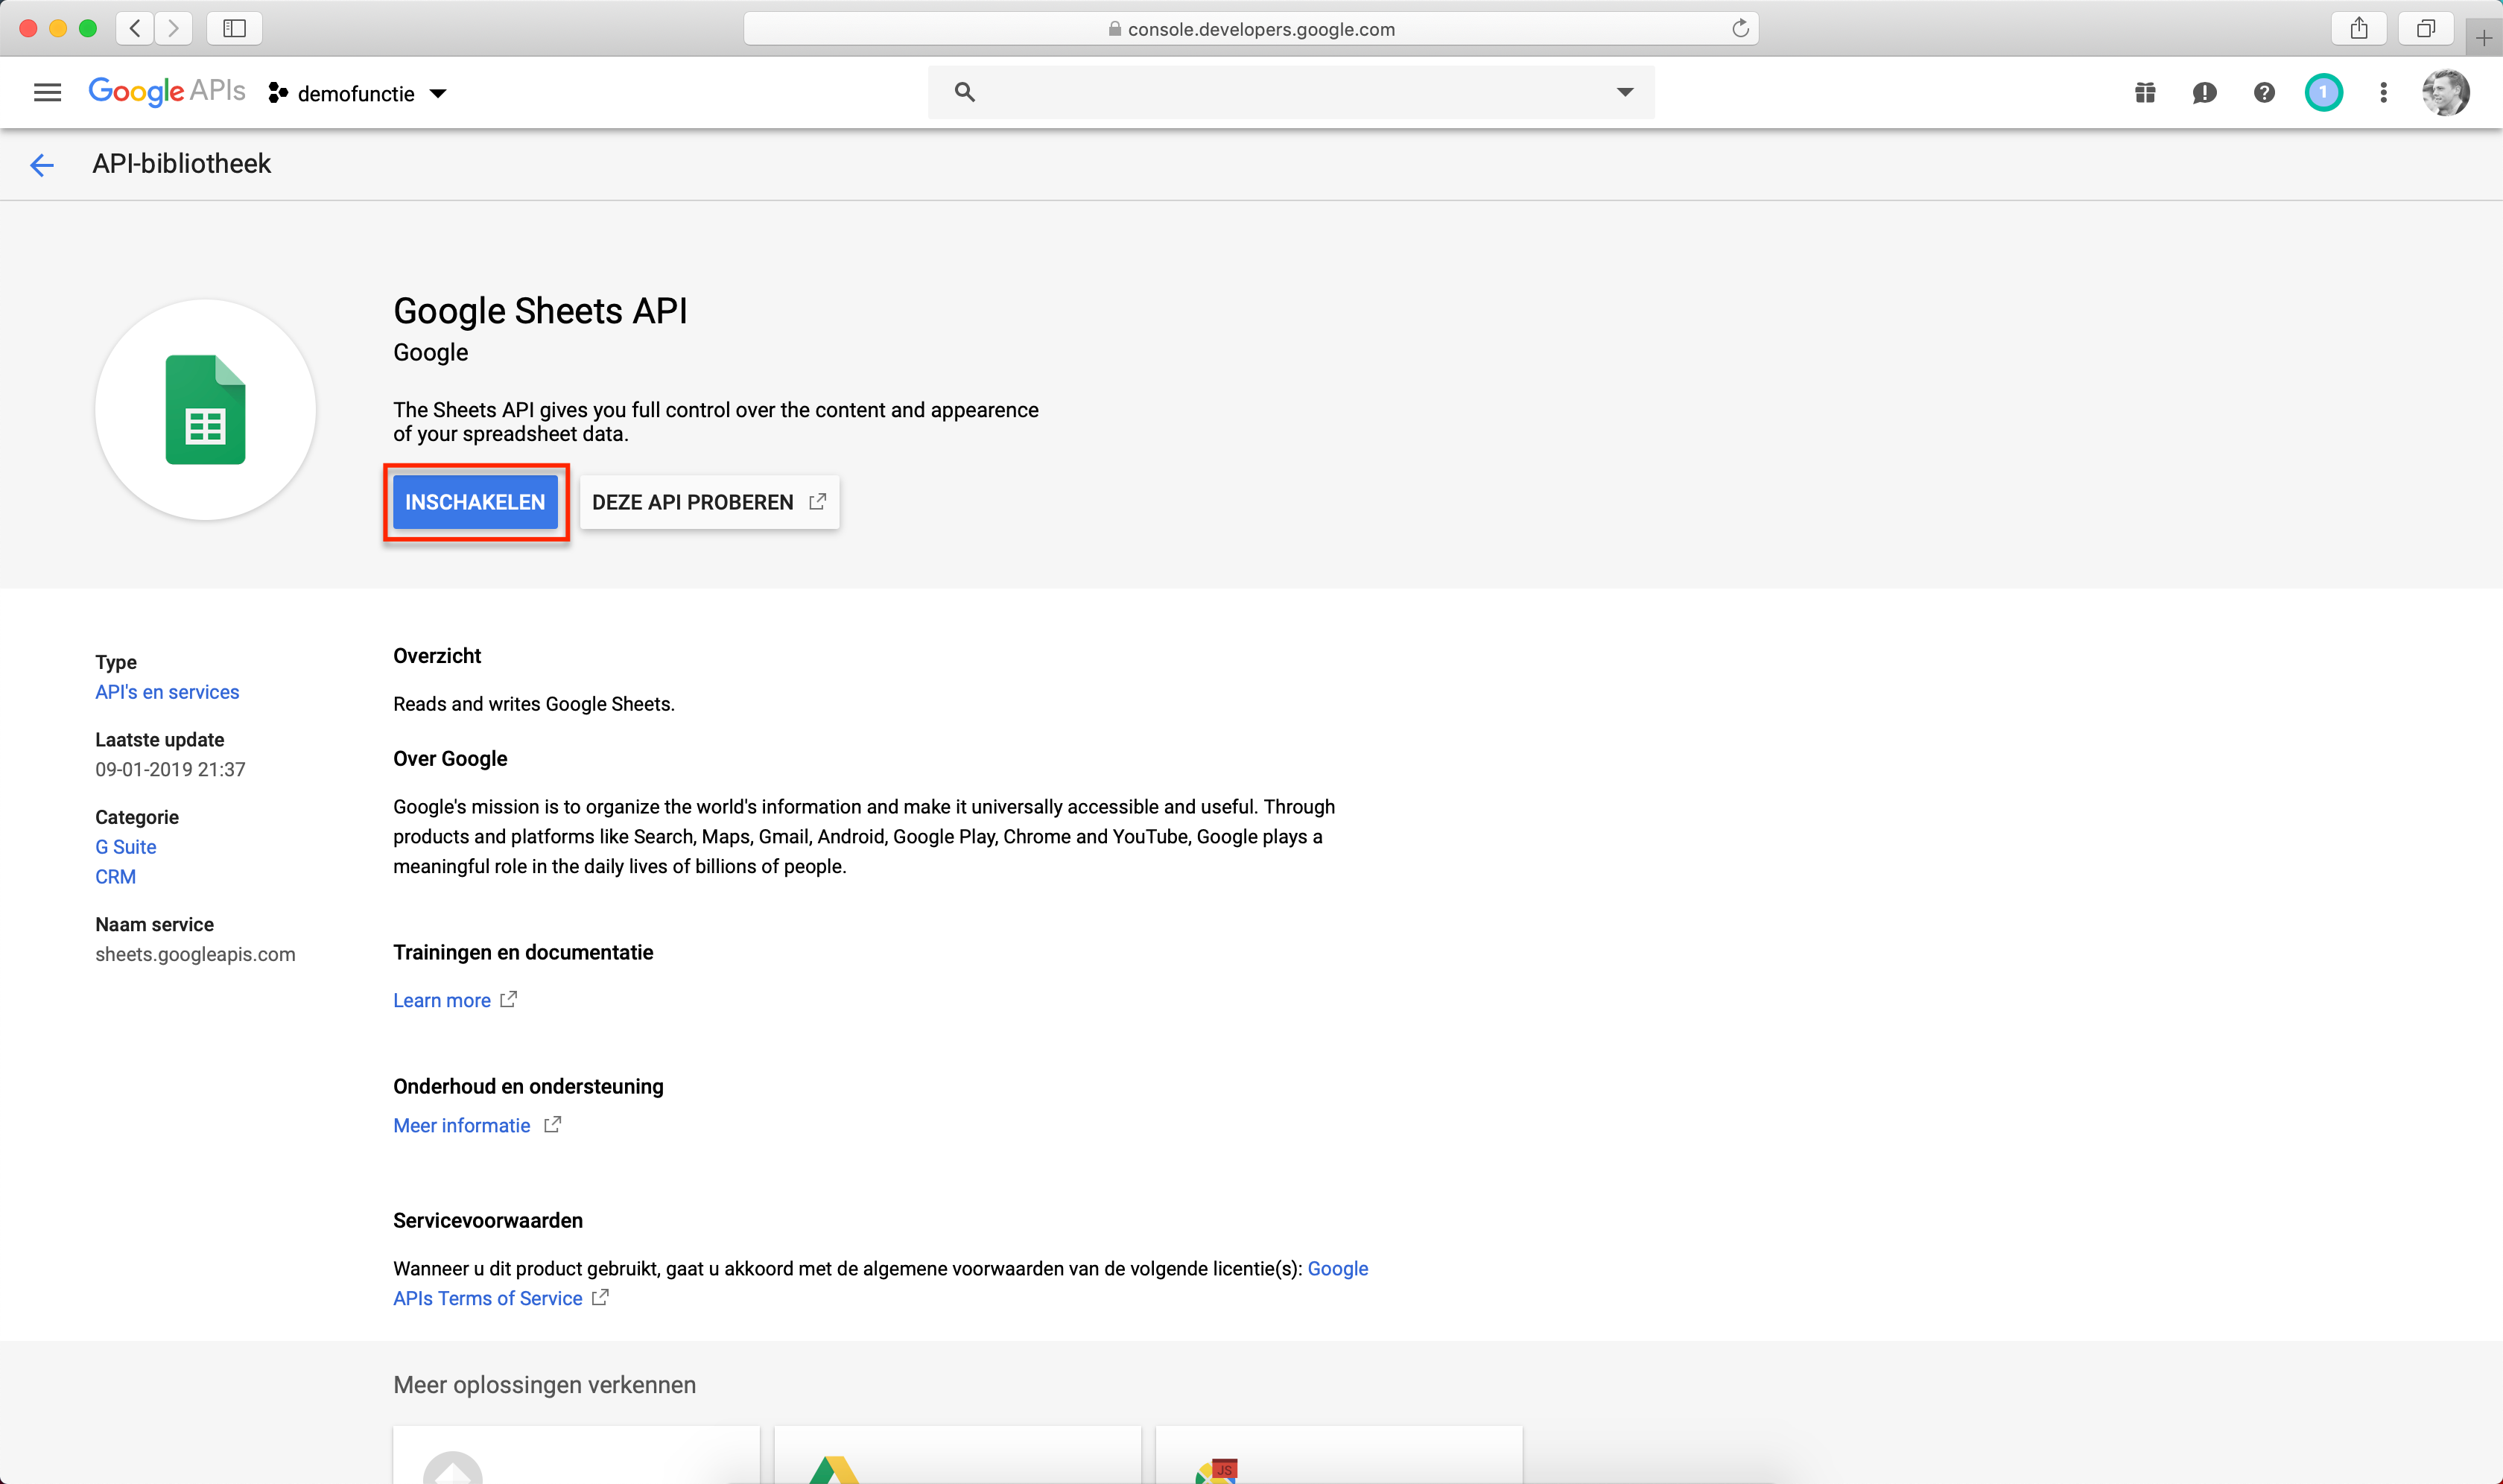
\includegraphics[width=0.9\linewidth,height=4.3cm]{img/google-sheets/gapi-google-sheets-api.png}
        \centering
        \caption{Zoek de Goolge sheets API en schakel deze in}
    \end{subfigure}
\end{figure}
\begin{figure}[h]\ContinuedFloat
    \begin{subfigure}{0.5\textwidth}
        \captionsetup{width=0.8\linewidth}
        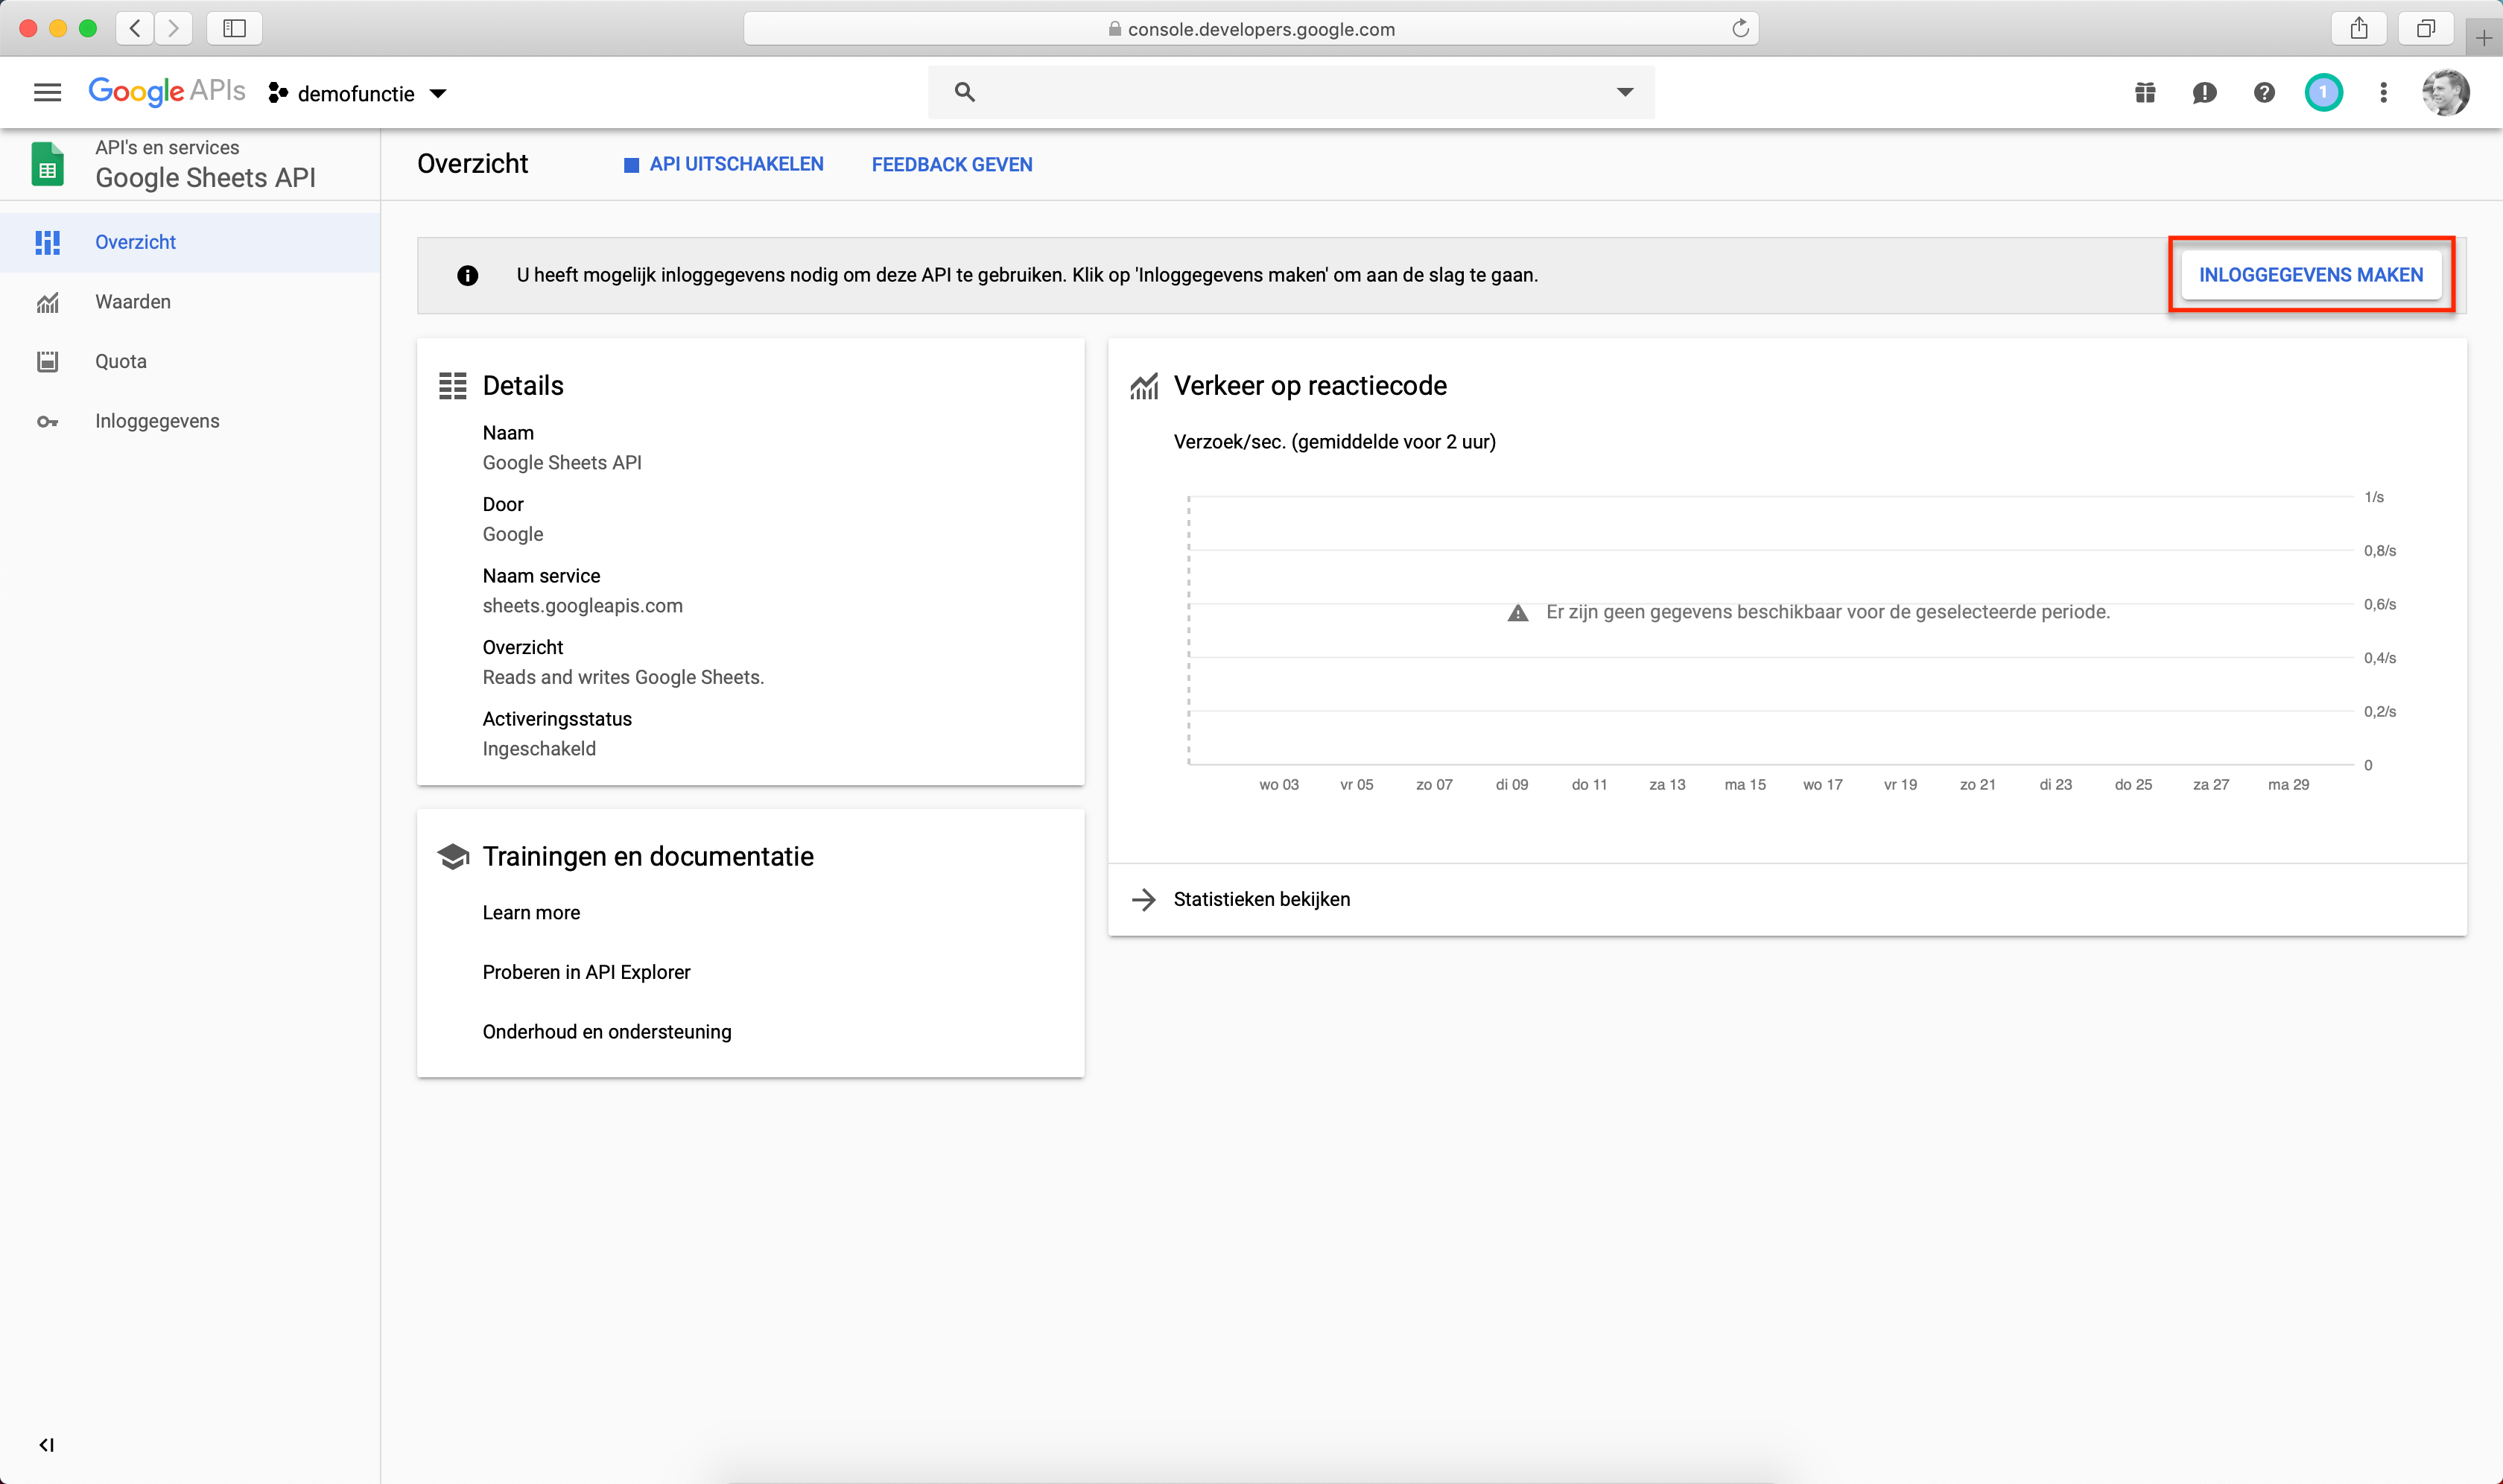
\includegraphics[width=0.9\linewidth,height=4.3cm]{img/google-sheets/gapi-maken-credentials.png}
        \centering
        \caption{Kies de optie om credentials aan te maken.}
    \end{subfigure}
    \begin{subfigure}{0.5\textwidth}
        \captionsetup{width=0.8\linewidth}
        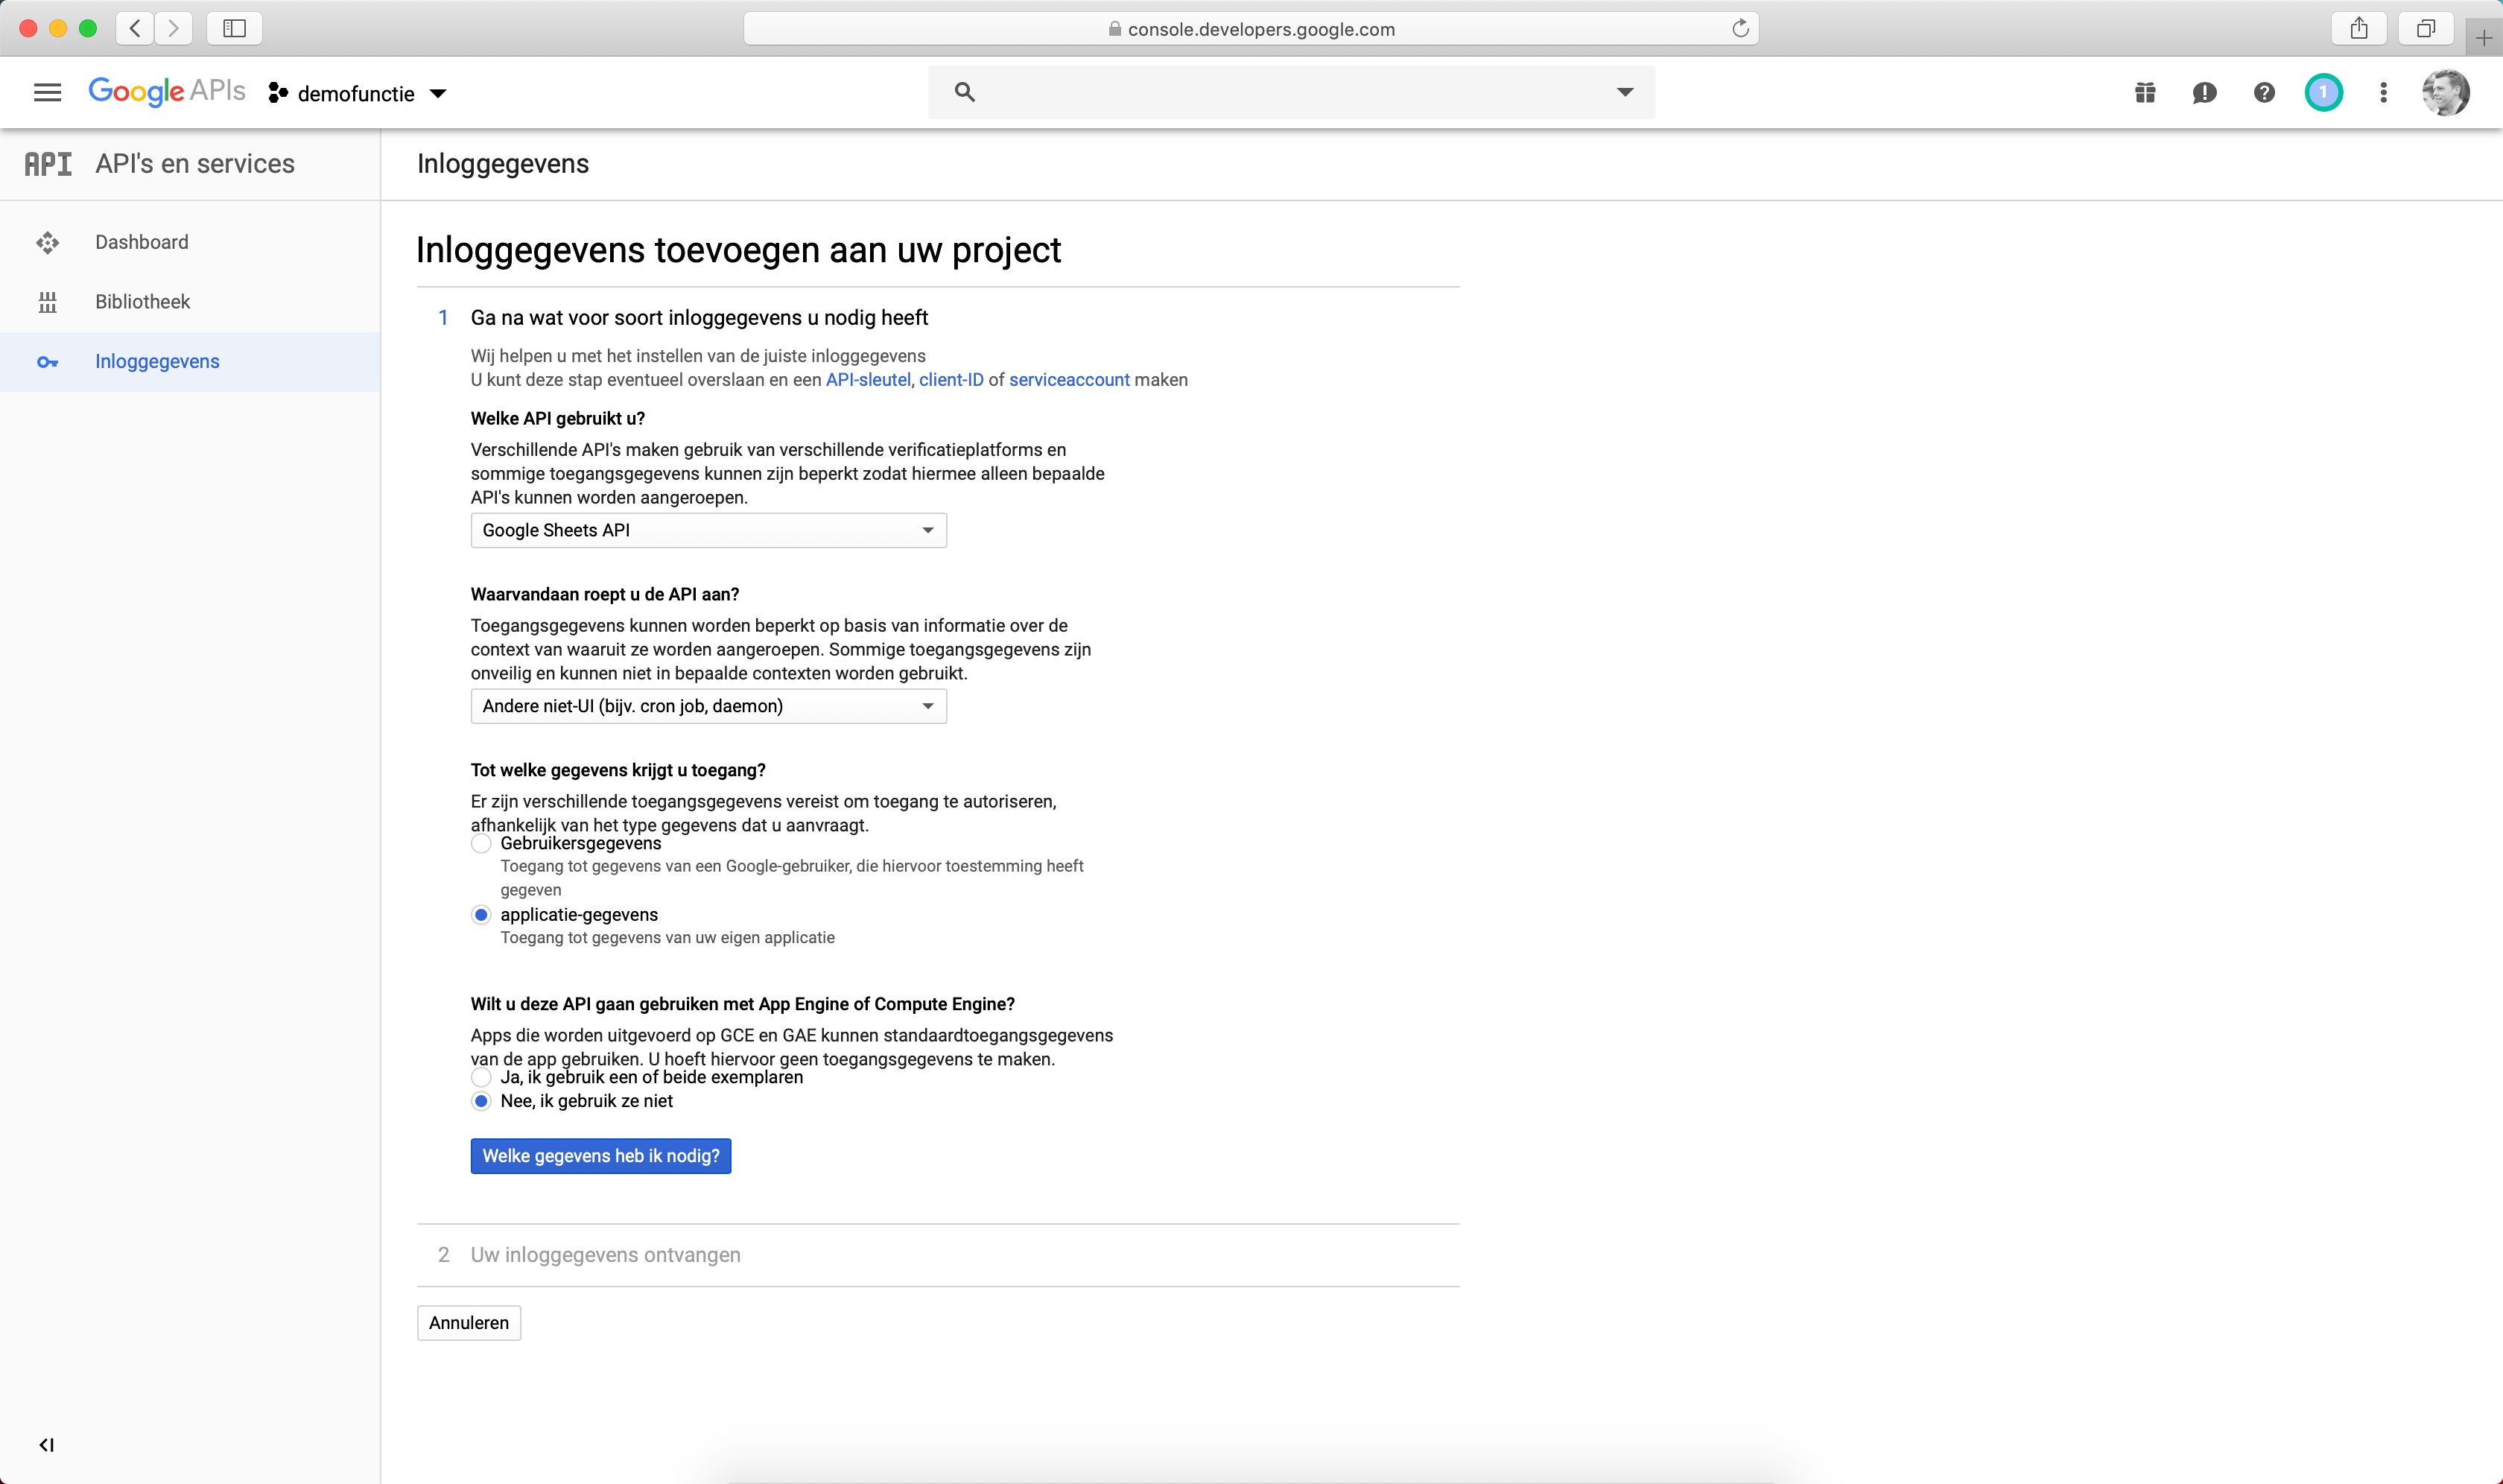
\includegraphics[width=0.9\linewidth,height=4.3cm]{img/google-sheets/gapi-credentials-1.png}
        \centering
        \caption{Invullen van gegevens voor credentials deel 1.}
    \end{subfigure}
\end{figure}
\begin{figure}[h]\ContinuedFloat
    \begin{subfigure}{0.5\textwidth}
        \captionsetup{width=0.8\linewidth}
        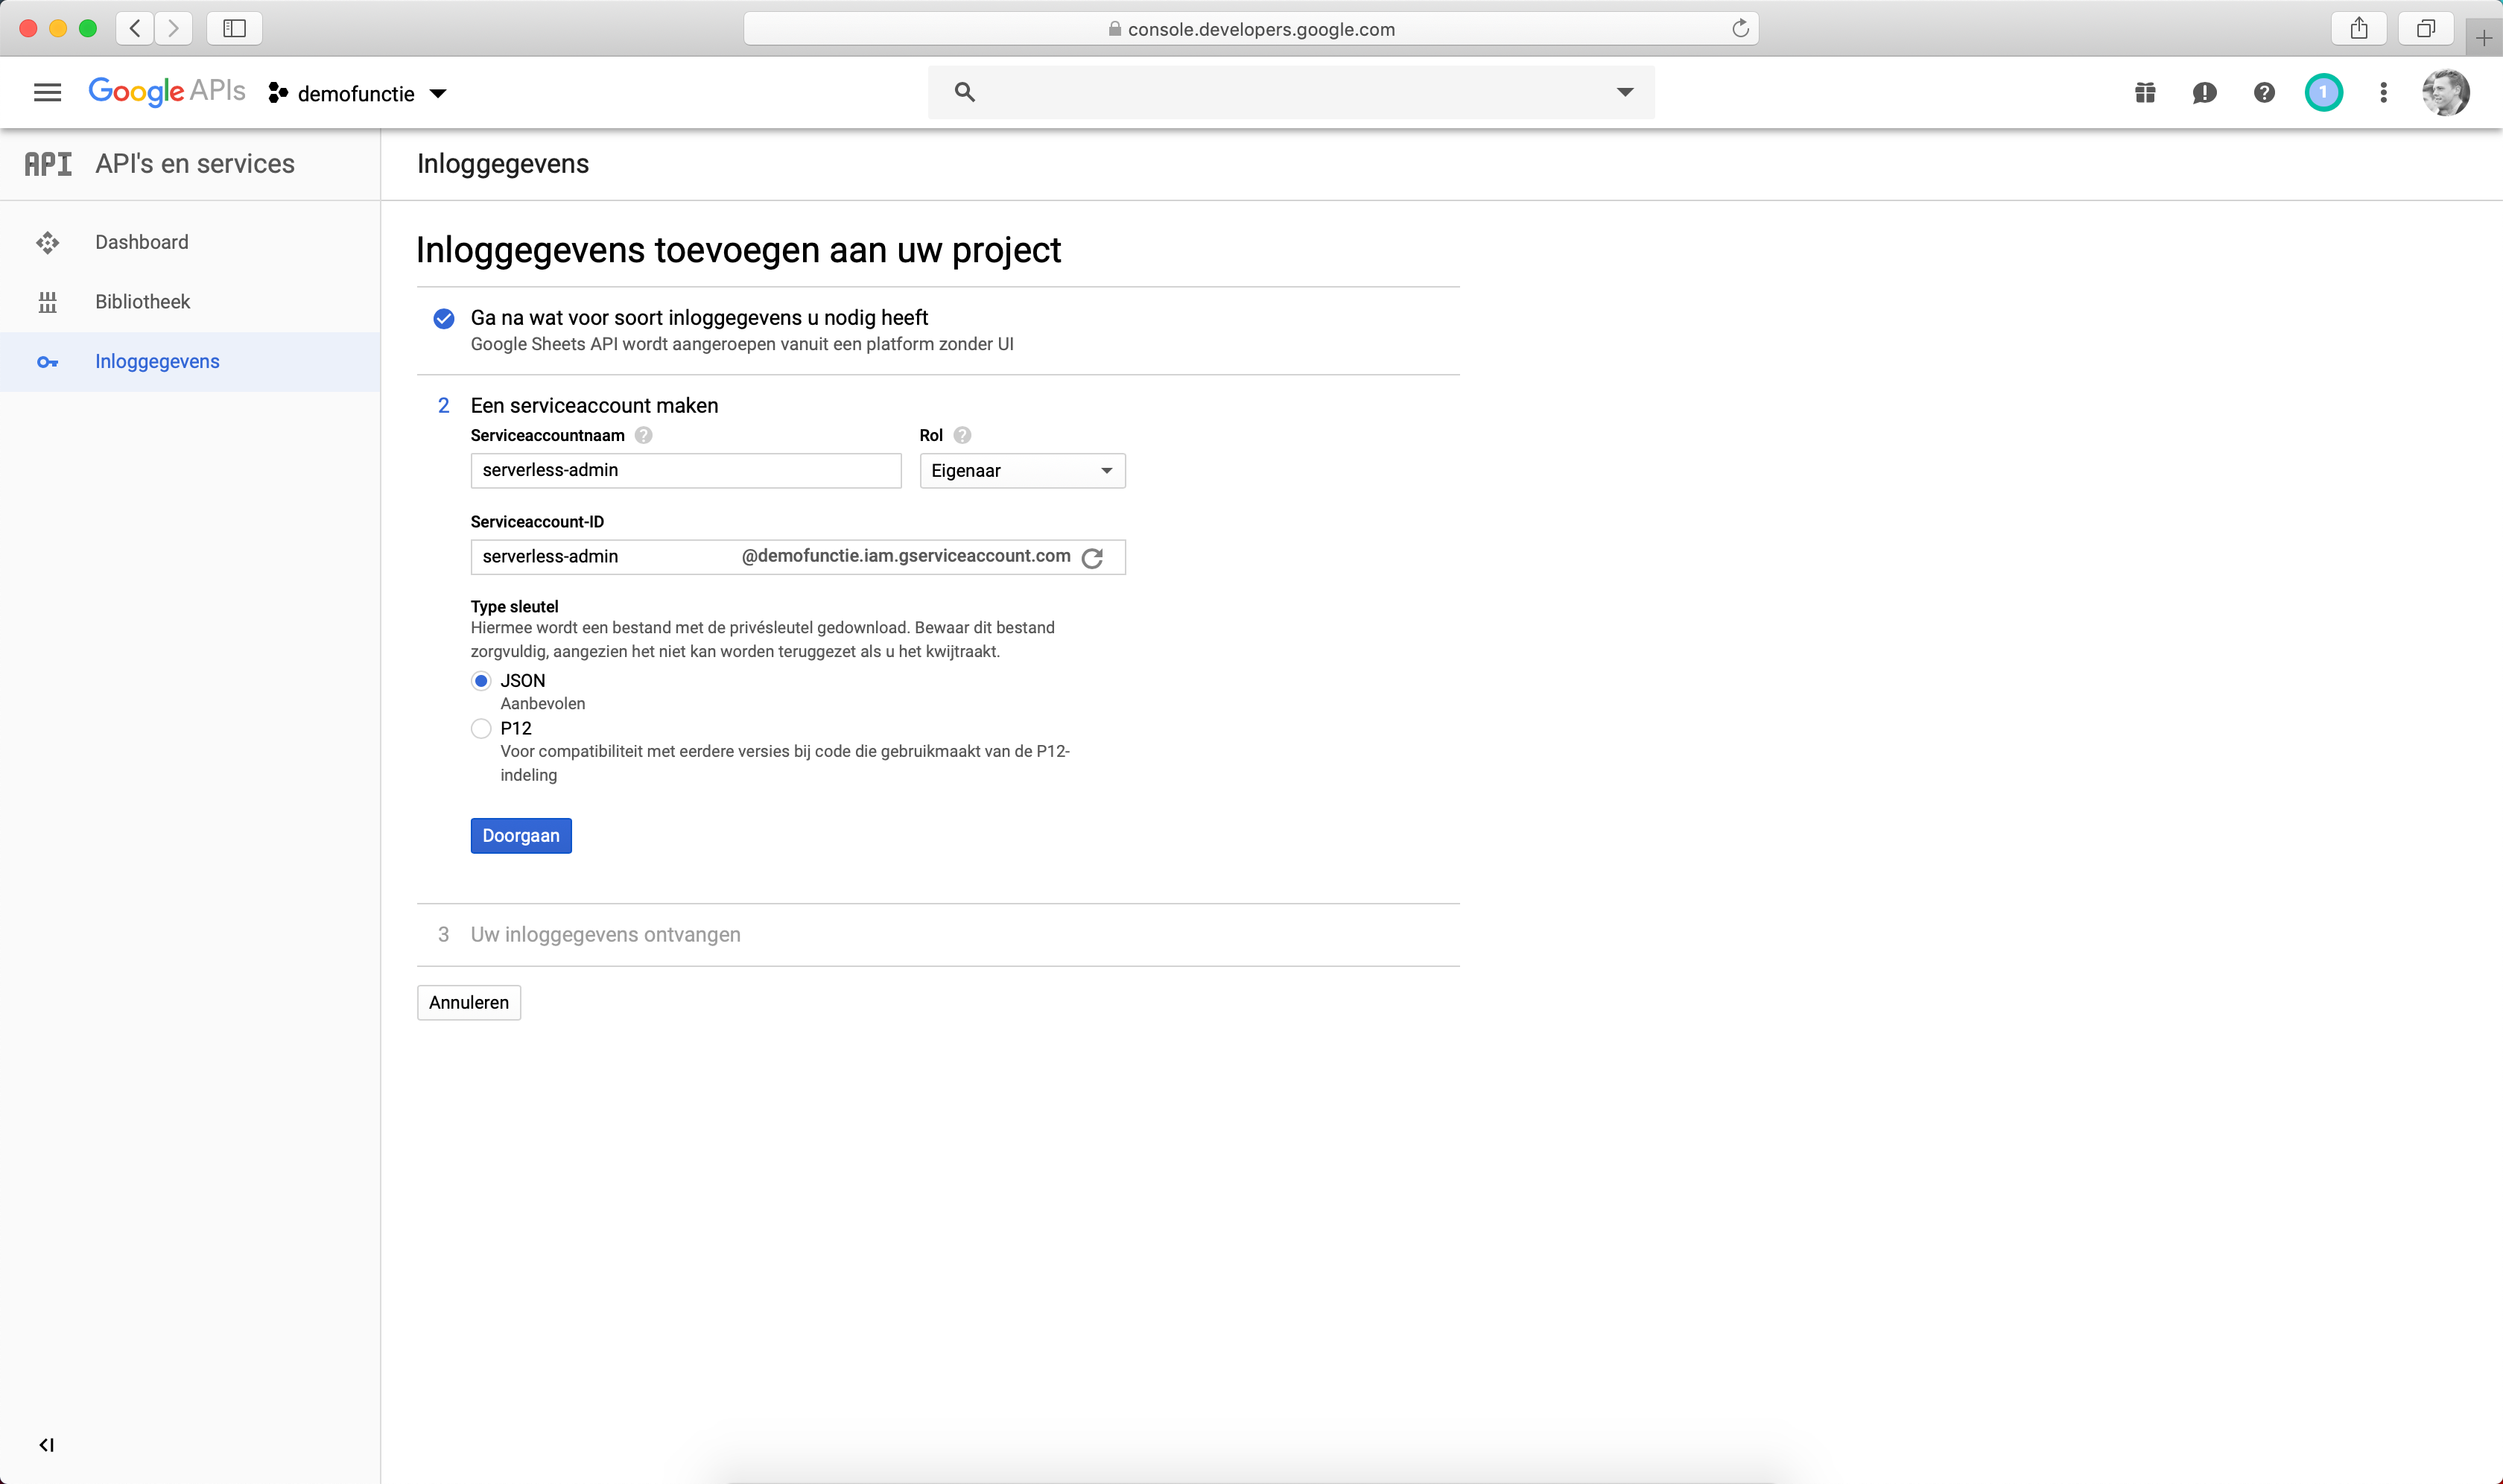
\includegraphics[width=0.9\linewidth,height=4.3cm]{img/google-sheets/gapi-credentials-2.png}
        \centering
        \caption{Invullen van gegevens voor credentials deel 2.}
    \end{subfigure}
    \begin{subfigure}{0.5\textwidth}
        \captionsetup{width=0.8\linewidth}
        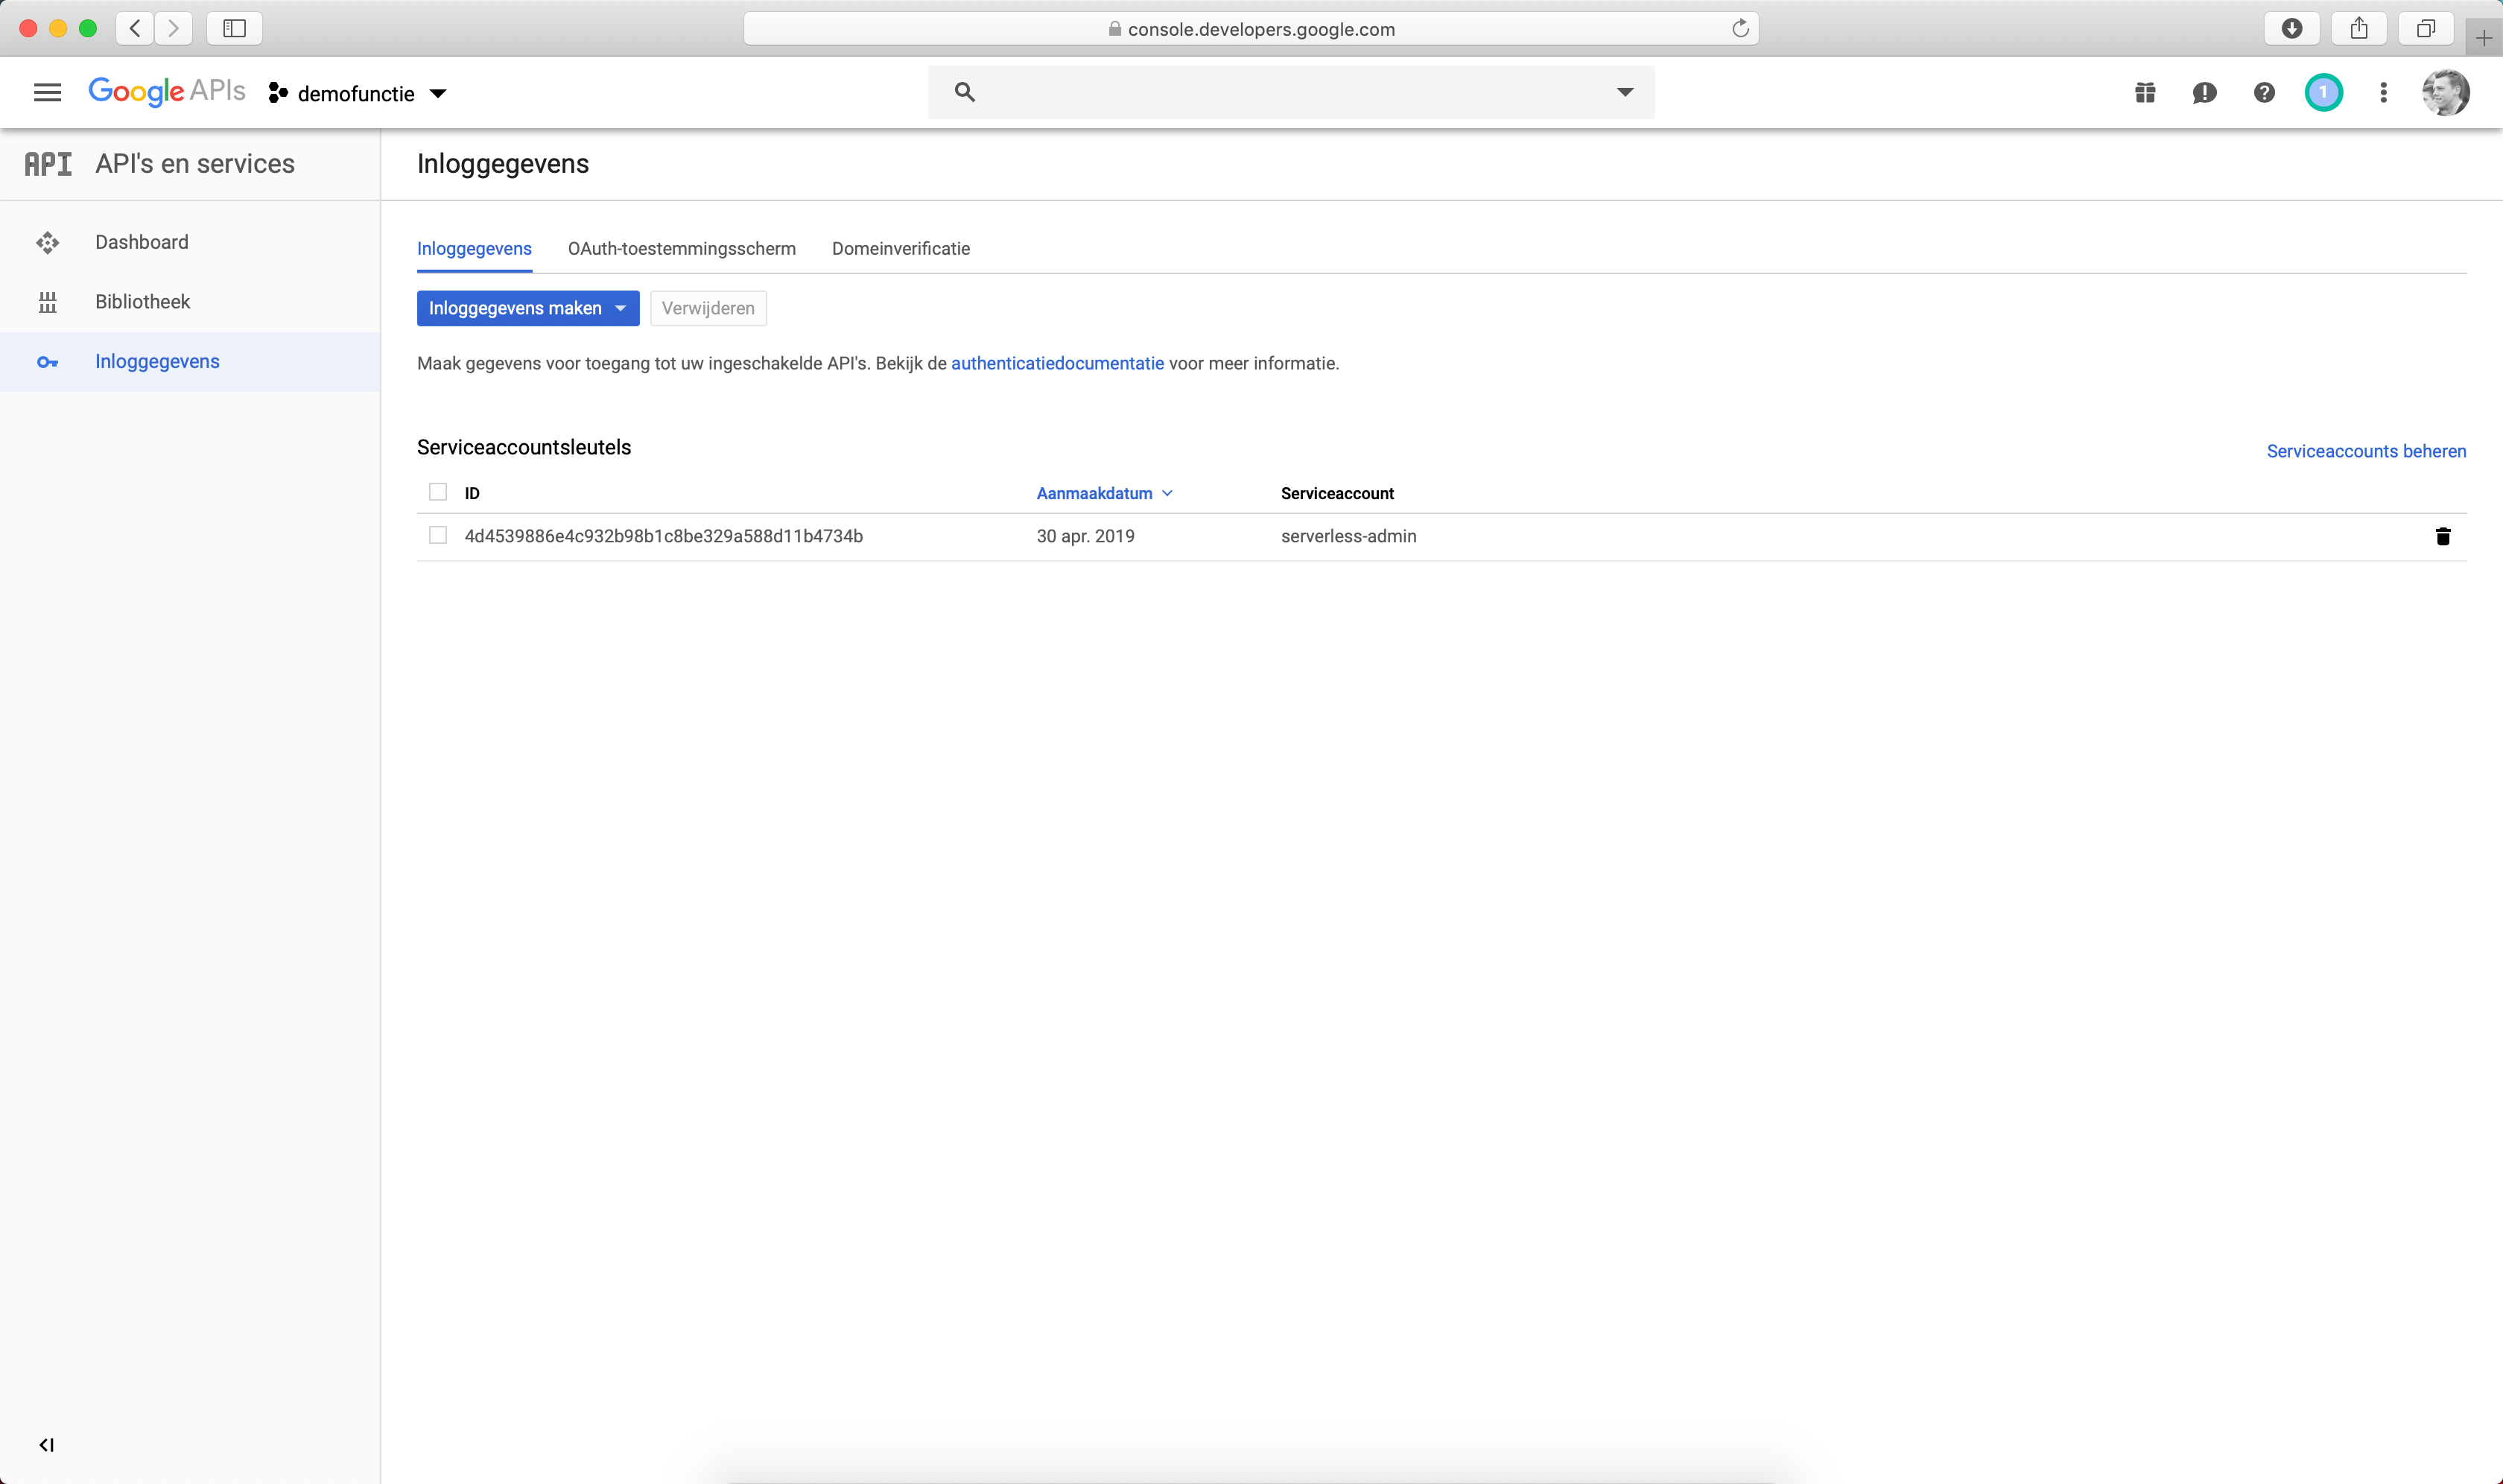
\includegraphics[width=0.9\linewidth,height=4.3cm]{img/google-sheets/gapi-credentials-3.png}
        \centering
        \caption{Credential account is nu beschikbaar.}
    \end{subfigure}
\end{figure}

Na het invullen van de gegevens voor het aanmaken van een credentials account wordt er automatisch een JSON bestand met de credential sleutel gedownload. Plaats dit bestand op een locatie waar het makkelijk is terug te vinden. Sla het bestand bijvoorbeeld op onder een map ''keys'' onder de home directory van de gebruiker en hernoem het naar ''credentials-serverless.json''. Maak vervolgens een nieuw Google spreadsheet\footnote{https://docs.google.com/spreadsheets} document aan en deel het bestand met de eerder aangemaakte gebruiker. Gebruik de ''client\_email'', deze is terug te vinden in het credentials bestand dat eerder werd gedownload. Nu is Google spreadsheets en de Sheets API correct geconfigureerd, Python heeft nu toegang tot de spreadsheet en kan nu data lezen en schrijven naar dit bestand.

\chapter{Issues}
\section{Issues}
\subsection{Fission Slack conversatie}
\label{sec:fission-slack-issue}
In afbeelding \ref{fig:fission-slack-issue-1} is de conversatie gevoerd op de Slack channel van het Fission project terug te vinden. Deze mensen hebben geprobeerd het probleem te verhelpen maar hebben het ook niet onmiddellijk gevonden.
\begin{figure}
    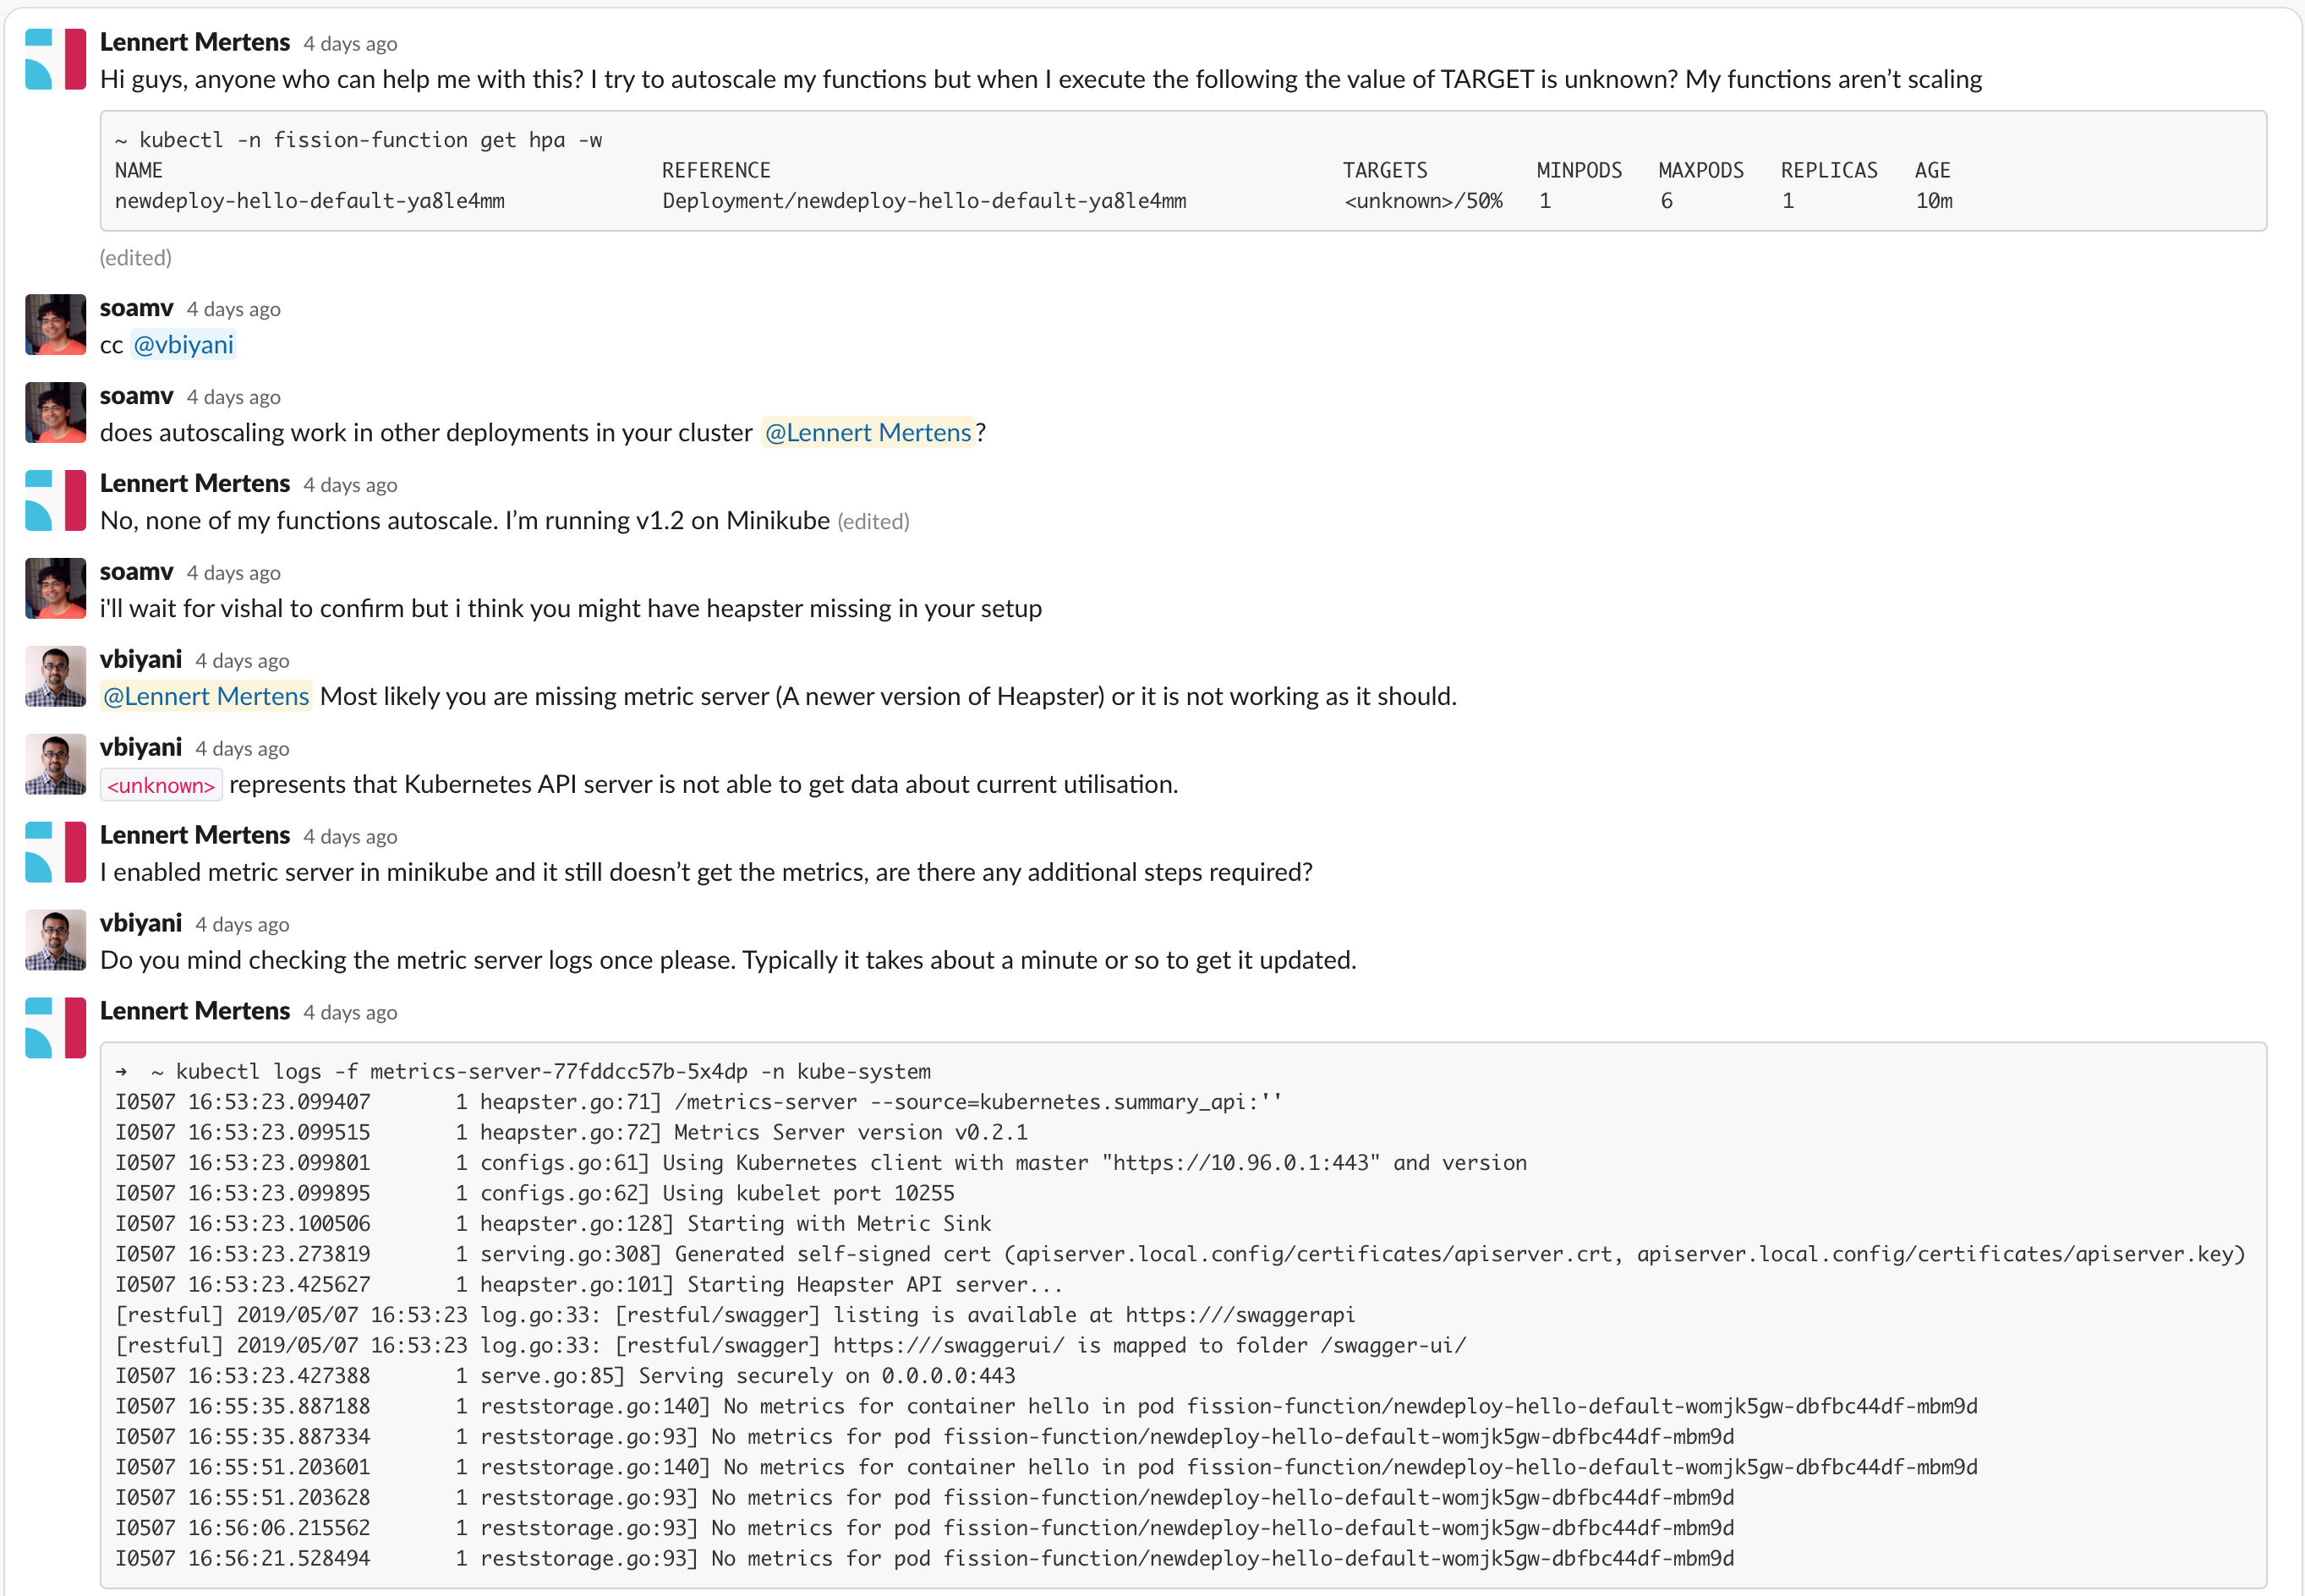
\includegraphics[width=1\textwidth]{img/fission-slack-issue-1.png}
     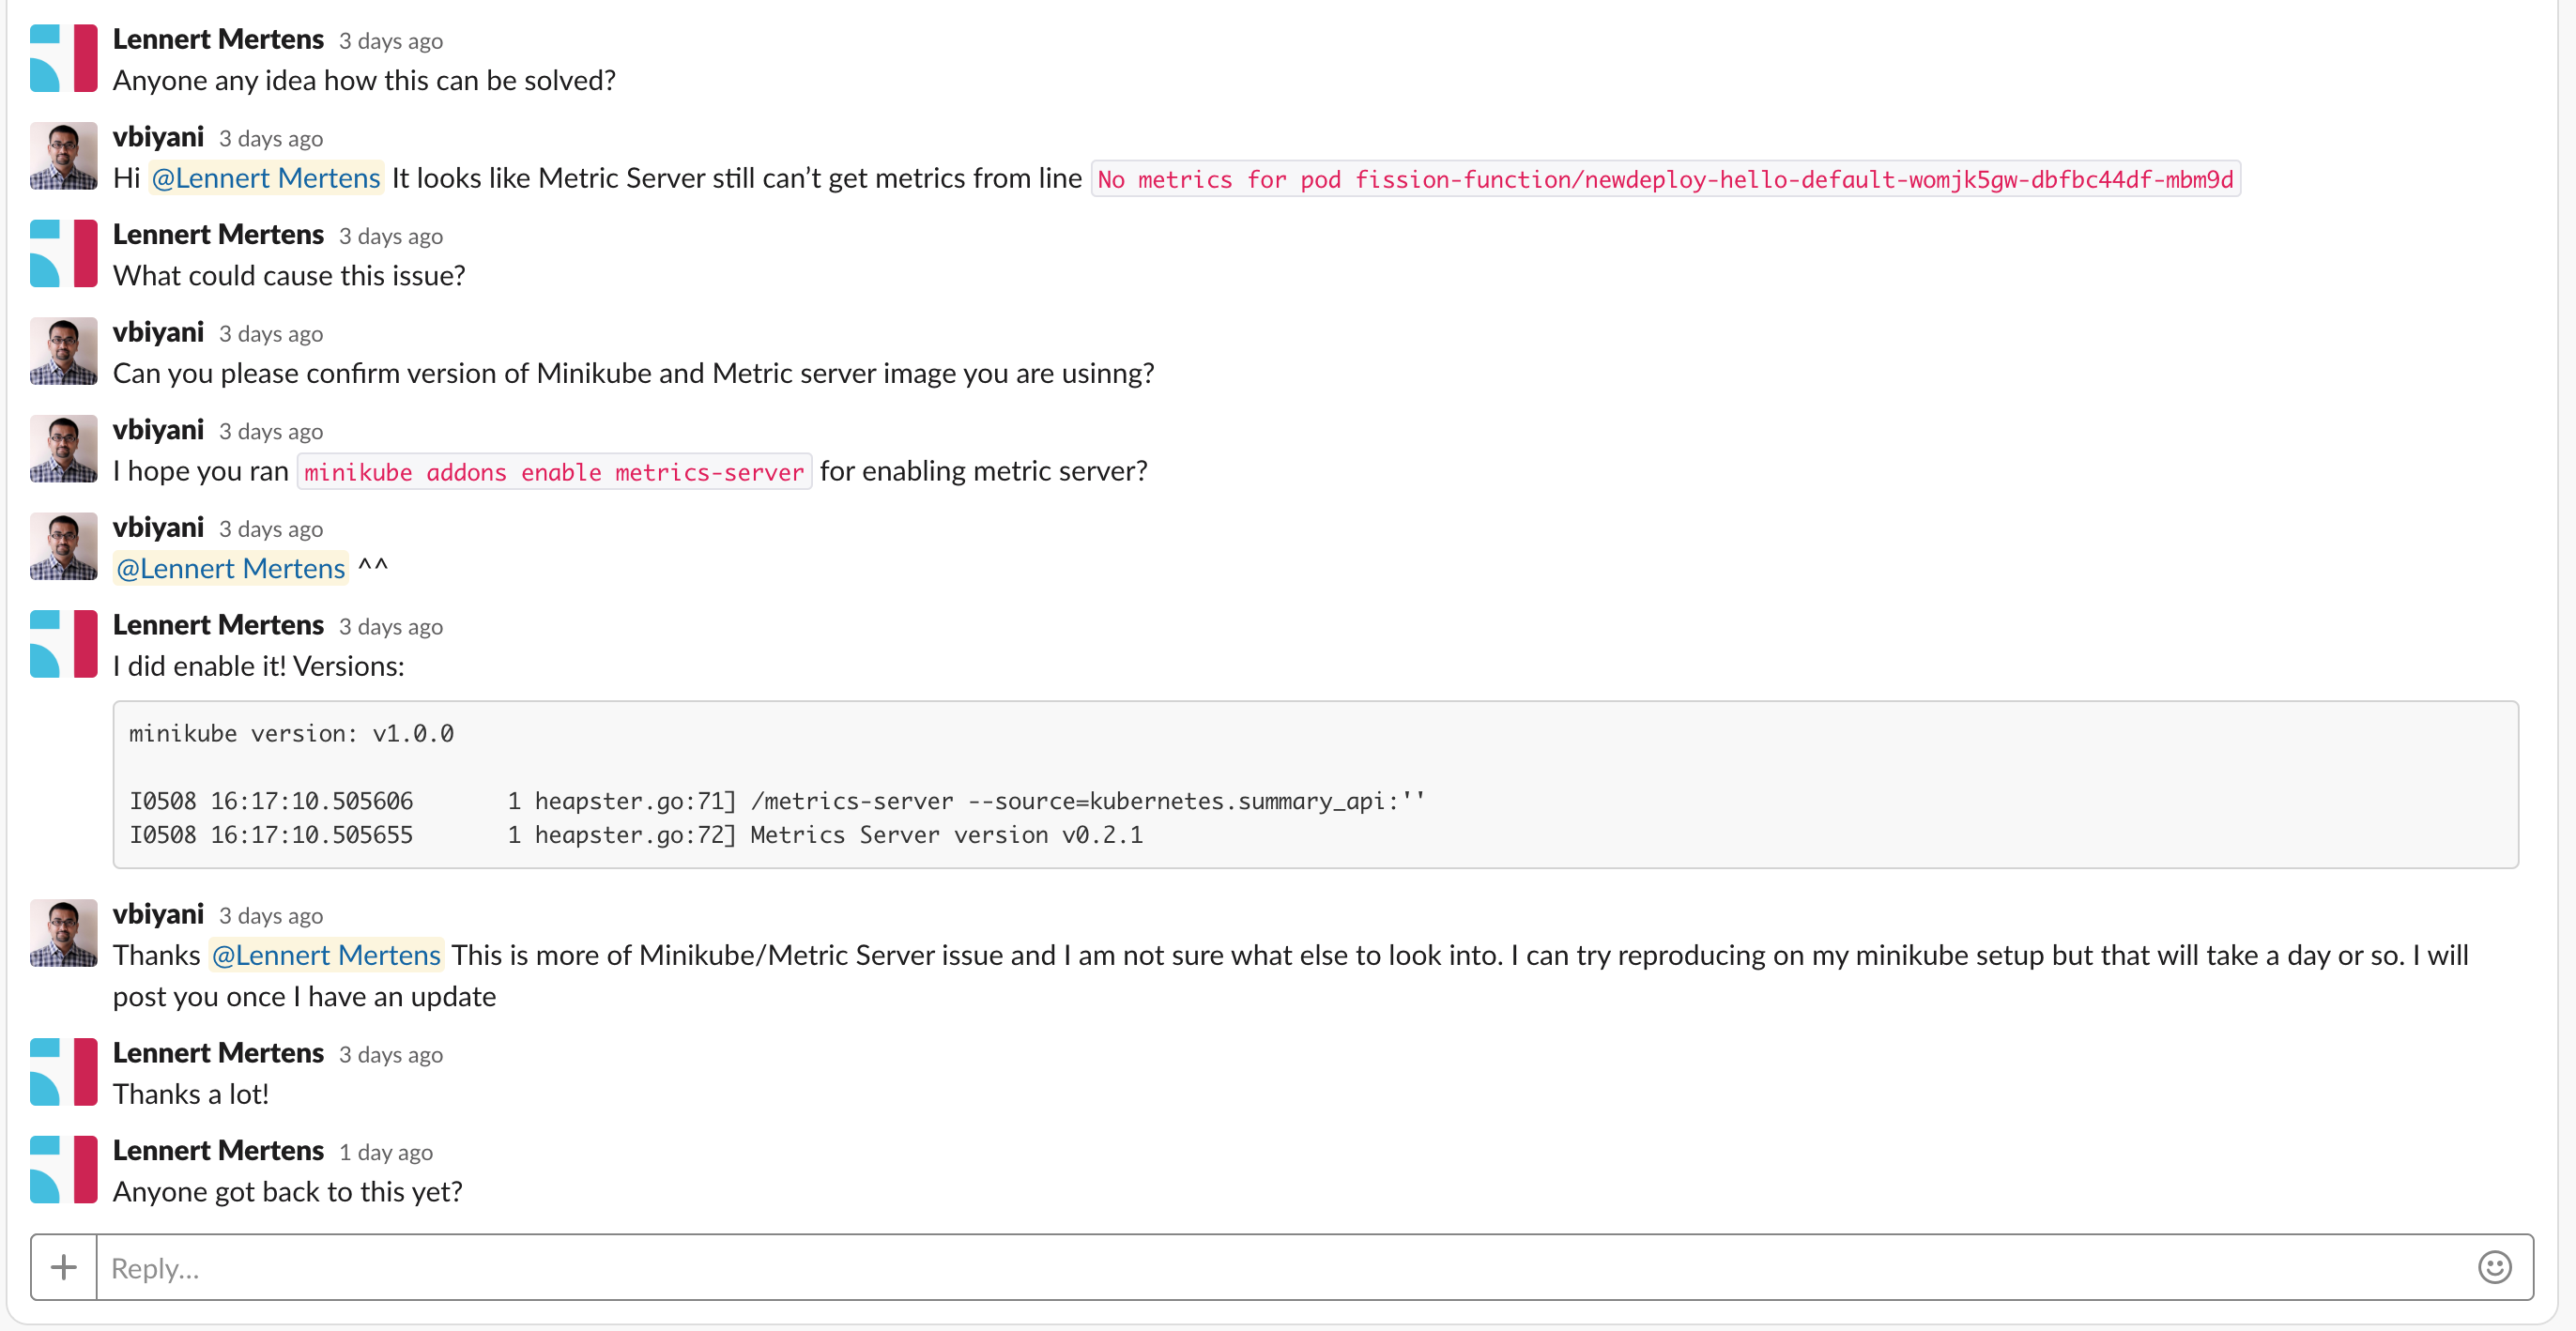
\includegraphics[width=1\textwidth]{img/fission-slack-issue-2.png}
    \caption{Fission functie target unknown.}
    \label{fig:fission-slack-issue-1}  
\end{figure}

\subsection{Fission GitHub issue}
\label{sec:fission-github-issue}
Na troubleshooting en verder uitproberen werd er besloten een GitHub issue\footnote{https://github.com/fission/fission/issues/1182} aan te maken op het Fission project en de tegengekomen problemen te melden, dit kan anderen die hetzelfde probleem tegenkomen helpen.
\begin{figure}
    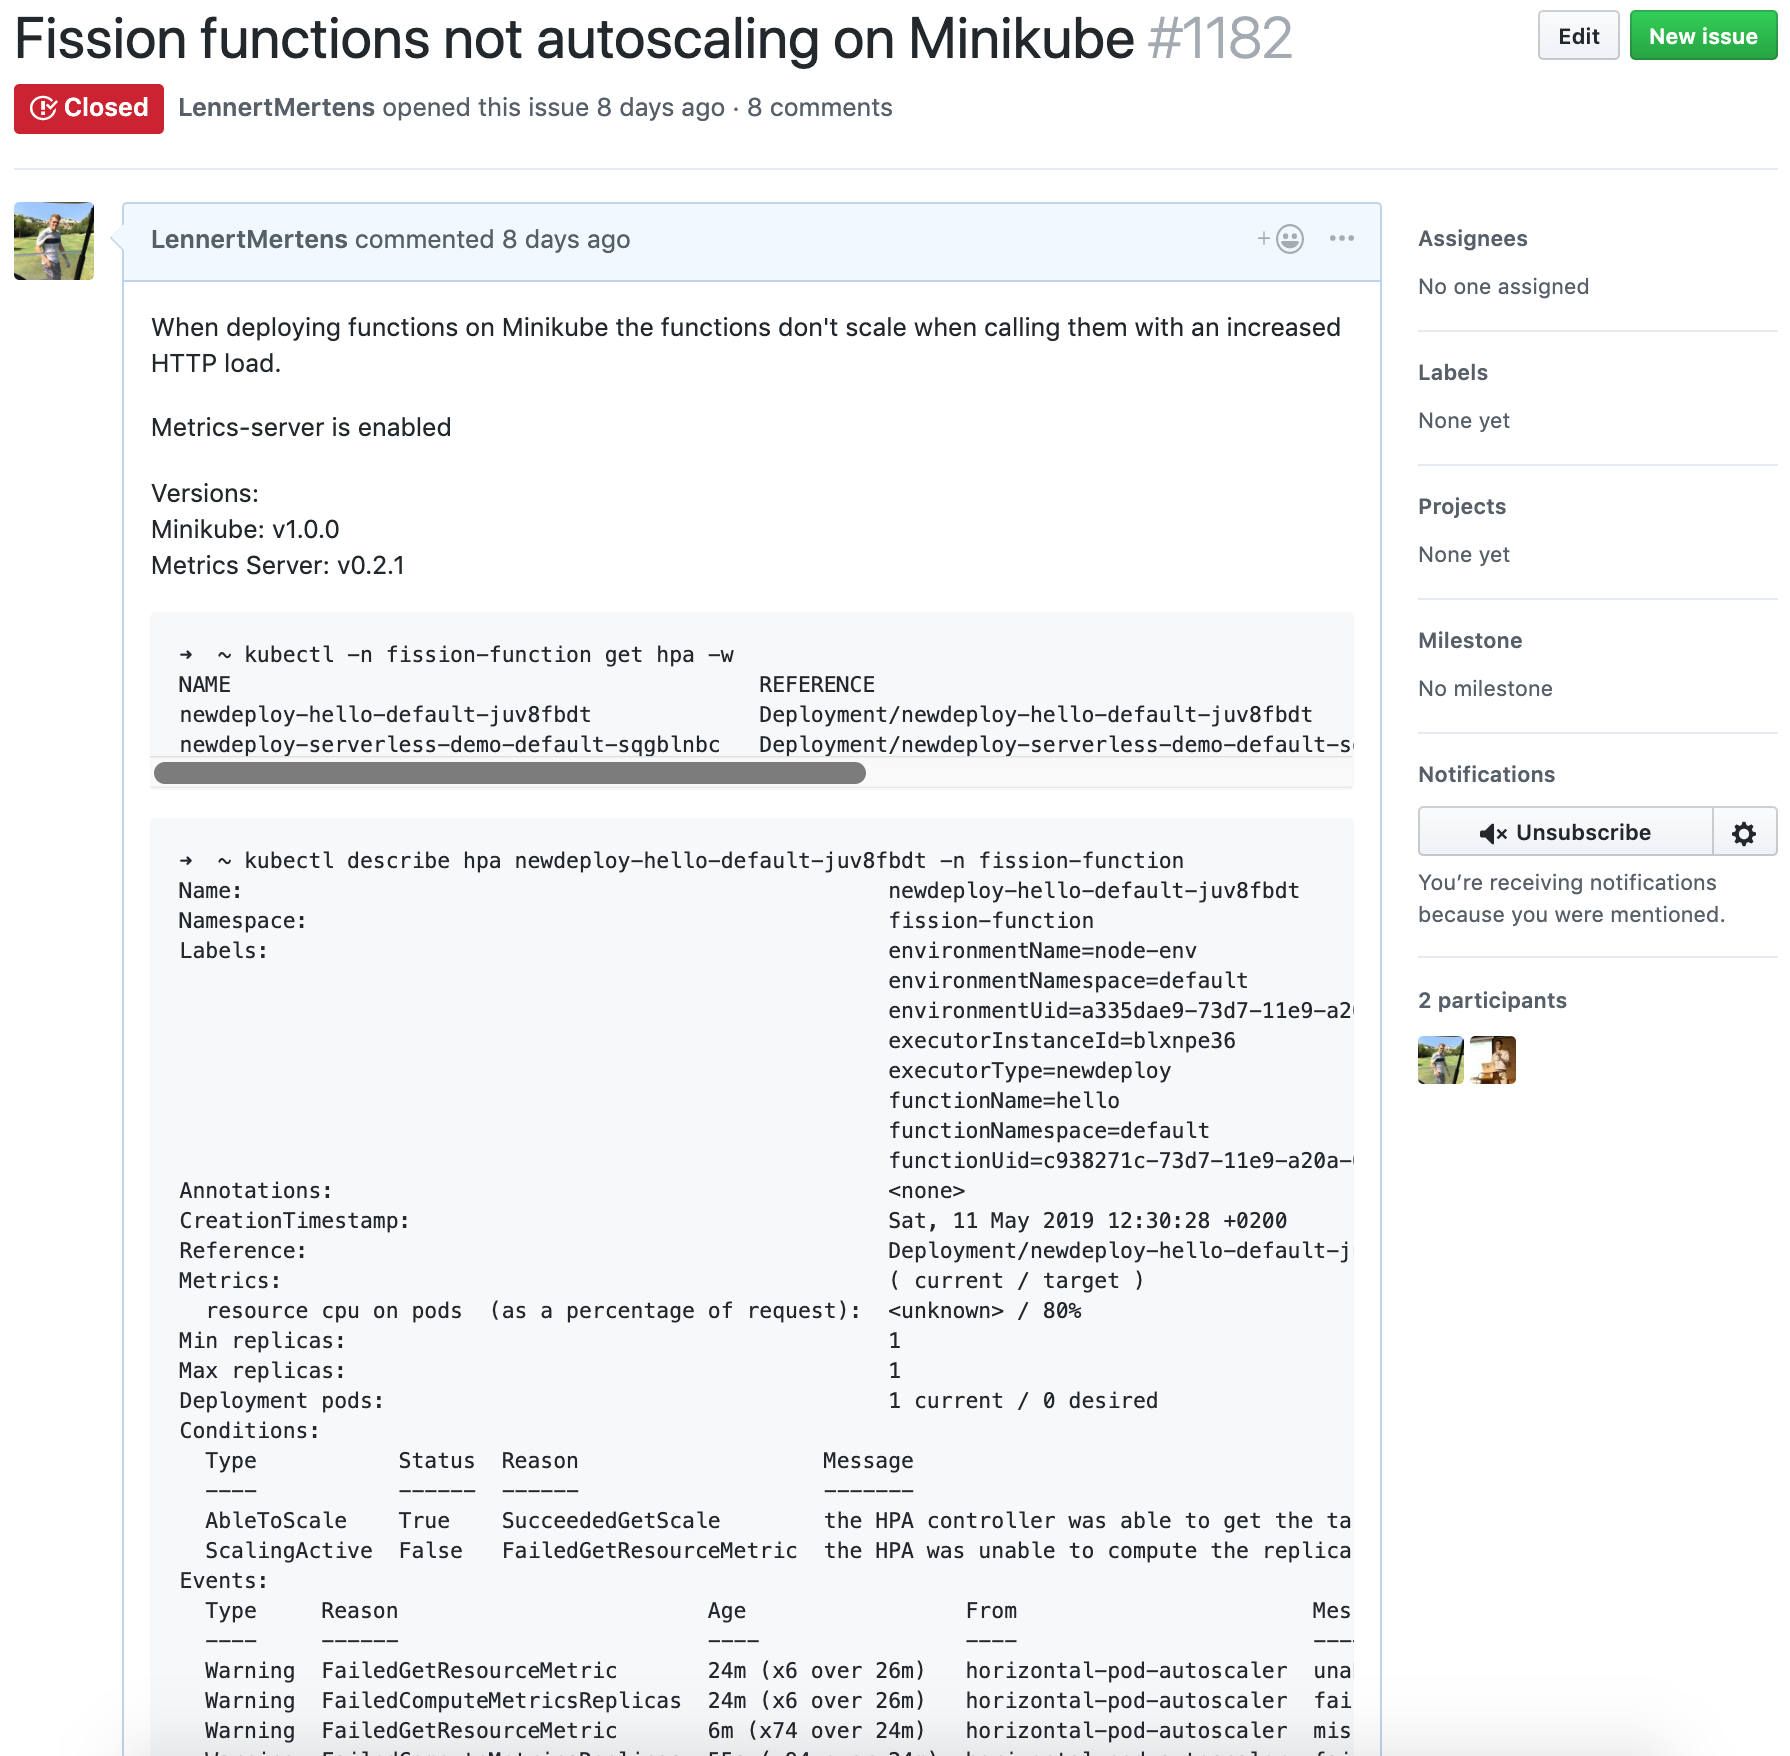
\includegraphics[width=1\textwidth]{img/fission-github-issue.png}
    \caption{Fission issue op GitHub.}
    \label{fig:fission-github-issue}  
\end{figure}
\chapter{Datasets}
\section{Datasets}
\subsection{Demofunctie uitvoeringstijd in seconden}
%%---------- Referentielijst --------------------------------------------------

\printbibliography[heading=bibintoc]
%\addcontentsline{toc}{chapter}{\textcolor{maincolor}{\IfLanguageName{dutch}{Bibliografie}{Bibliography}}}

\end{document}
